\documentclass{report}

% ====================================================
%       1. PACKAGES (ترتیب در لاتکس به شدت مهم است)
% ====================================================
\usepackage{graphicx}
\usepackage{subcaption}
\usepackage{fancyhdr}
\usepackage[margin=1in]{geometry}
\usepackage{amsmath,amssymb,mathtools}
\usepackage{float}
\usepackage{lmodern}
\usepackage{xcolor}
\usepackage{listings}
\usepackage{fvextra}
\usepackage{longtable}
\usepackage{enumitem}
\usepackage{booktabs}
\usepackage{array}
\usepackage{multirow}
\usepackage{colortbl}
\usepackage{titlesec}
\usepackage{tikz}
\usepackage{eso-pic} 
\usepackage[most]{tcolorbox}
\usetikzlibrary{calc, shadows.blur} 

% هایپررف حتماً باید قبل از زی‌پرشین باشد
\usepackage[hidelinks]{hyperref} 

% زی‌پرشین حتماً حتماً باید آخرین پکیج باشد
\usepackage{xepersian}

% ====================================================
%       2. FONTS
% ====================================================
\settextfont[Path={./font/}, Scale=1.4]{IRLotus}
\setlatintextfont[Scale=1.1]{Times New Roman}

% ====================================================
%       3. COLORS 
% ====================================================
\definecolor{mainblue}{RGB}{15,76,129}
\definecolor{lightblue}{RGB}{226,238,250}
\definecolor{deepblue}{RGB}{9,24,51} 

% --- رنگ‌های جدید تم کلاسیک و پلاتینی صفحه اول ---
\definecolor{midnight}{RGB}{8, 12, 20}         % سورمه‌ای/مشکی بسیار تاریک و عمیق
\definecolor{platinum}{RGB}{214, 219, 223}     % نقره‌ای روشن و شیک برای متن و لبه‌ها
\definecolor{mutedslate}{RGB}{69, 84, 104}     % خاکستری متمایل به آبی برای فریم‌ها و کادرها
\definecolor{slatebg}{RGB}{20, 30, 45}          % سورمه‌ای-زغالی عمیق و مات

\definecolor{softgray}{RGB}{245,245,245}

% تم کادرهای مات
\definecolor{mattedarkblue}{RGB}{35, 45, 60} 
\definecolor{mattebgblue}{RGB}{248, 250, 253} 
\definecolor{mattedarkgold}{RGB}{120, 95, 45} 
\definecolor{mattebggold}{RGB}{254, 253, 249} 
\definecolor{mattedarkred}{RGB}{100, 35, 40} 
\definecolor{mattebgred}{RGB}{253, 248, 248} 

% رنگ‌های تم VS Code Dark+
\definecolor{vscBackground}{RGB}{30,30,30}      
\definecolor{vscText}{RGB}{212,212,212}         
\definecolor{vscPink}{RGB}{197,134,192}         
\definecolor{vscBlue}{RGB}{86,156,214}          
\definecolor{vscString}{RGB}{206,145,120}       
\definecolor{vscComment}{RGB}{106,153,85}       
\definecolor{vscTopBar}{RGB}{37,37,38}          

% ====================================================
%       4. VS CODE STYLE DEFINITION
% ====================================================

% --- استایل پایتون (همان استایل قبلی) ---
\lstdefinestyle{vscode_inner}{
    language=Python,
    backgroundcolor=\color{vscBackground},
    basicstyle=\linespread{1.1}\ttfamily\footnotesize\color{vscText}, 
    commentstyle=\color{vscComment}\itshape,
    stringstyle=\color{vscString},
    numberstyle=\tiny\color{gray}, 
    breakatwhitespace=false,
    breaklines=true,
    keepspaces=true,
    numbers=left,
    numbersep=12pt, 
    showspaces=false,
    showstringspaces=false,
    showtabs=false,
    tabsize=4,
    frame=none, 
    xleftmargin=12pt,
    morestring=[s]{"""}{"""},
    morestring=[s]{'''}{'''},
    classoffset=0,
    morekeywords={def,for,in,return,class,if,else,elif,while,try,except,with,and,or,not,is,yield,global},
    keywordstyle=\color{vscPink}\bfseries,
    classoffset=1,
    morekeywords={import,as,from,True,False,None,self,pass,print},
    keywordstyle=\color{vscBlue}\bfseries,
    classoffset=0, 
}

% --- استایل متلب (جدید) ---
\lstdefinestyle{vscode_inner_matlab}{
    language=MATLAB,
    backgroundcolor=\color{vscBackground},
    basicstyle=\linespread{1.1}\ttfamily\footnotesize\color{vscText},
    commentstyle=\color{vscComment}\itshape,
    stringstyle=\color{vscString},
    numberstyle=\tiny\color{gray},
    breakatwhitespace=false,
    breaklines=true,
    keepspaces=true,
    numbers=left,
    numbersep=12pt,
    showspaces=false,
    showstringspaces=false,
    showtabs=false,
    tabsize=4,
    frame=none,
    xleftmargin=12pt,
    morestring=[s]{'}{'},
    morestring=[s]{"}{"},
    comment=[l]{\%},
    classoffset=0,
    morekeywords={if,else,elseif,for,while,switch,case,otherwise,function,
                  return,break,continue,end,global,persistent,try,catch,
                  classdef,properties,methods,events,enumeration,parfor,spmd,using},
    keywordstyle=\color{vscPink}\bfseries,
    classoffset=1,
    morekeywords={disp,eig,ss,tf,acker,ctrb,obsv,rank,step,plot,figure,
                  title,legend,xlabel,ylabel,grid,hold,subplot,zeros,ones,eye,
                  size,length,num2str,strcat,sprintf,fprintf,input,load,save,
                  clear,clc,close,all,any,find,sum,mean,std,max,min,abs,sqrt,
                  exp,log,sin,cos,tan,atan,real,imag,conj,angle,fft,ifft,
                  filter,tf2ss,ss2tf,damp,pzmap,dcgain,lsim,initial,impulse,
                  ode45,ode23,integral,quad,lsqnonlin,fmincon,optimoptions},
    keywordstyle=\color{vscBlue}\bfseries,
    classoffset=2,
    morekeywords={true,false,NaN,Inf,pi,i,j,eps},
    keywordstyle=\color{vscBlue}\bfseries,
    classoffset=0,
}

% --- محیط‌های نمایش کد (هر دو) ---
\newtcblisting{vscodewindow}[1]{
    enhanced,
    listing only,
    listing options={style=vscode_inner},
    title={\tikz[baseline=-0.6ex]{\fill[red!80!white] (0,0) circle (3.5pt); \fill[yellow!90!black] (0.4,0) circle (3.5pt); \fill[green!80!black] (0.8,0) circle (3.5pt);} \hspace{10pt} \ttfamily\footnotesize #1}, 
    fonttitle=\sffamily,
    coltitle=white,
    colbacktitle=vscTopBar, 
    colframe=vscTopBar, 
    colback=vscBackground,
    coltext=vscText, 
    arc=5mm, 
    outer arc=5mm,
    boxrule=1pt,
    titlerule=0pt, 
    toptitle=3mm, 
    bottomtitle=3mm,
    top=3mm, 
    bottom=3mm,
    left=2mm,
    right=2mm,
    drop shadow=black!50!white, 
    before skip=15pt,
    after skip=15pt
}

\newtcblisting{vscodewindowmatlab}[1]{
    enhanced,
    listing only,
    listing options={style=vscode_inner_matlab},
    title={\tikz[baseline=-0.6ex]{\fill[red!80!white] (0,0) circle (3.5pt); \fill[yellow!90!black] (0.4,0) circle (3.5pt); \fill[green!80!black] (0.8,0) circle (3.5pt);} \hspace{10pt} \ttfamily\footnotesize #1},
    fonttitle=\sffamily,
    coltitle=white,
    colbacktitle=vscTopBar,
    colframe=vscTopBar,
    colback=vscBackground,
    coltext=vscText,
    arc=5mm,
    outer arc=5mm,
    boxrule=1pt,
    titlerule=0pt,
    toptitle=3mm,
    bottomtitle=3mm,
    top=3mm,
    bottom=3mm,
    left=2mm,
    right=2mm,
    drop shadow=black!50!white,
    before skip=15pt,
    after skip=15pt
}

% ====================================================
%       5. GENERAL FORMATTING
% ====================================================

\hypersetup{
    colorlinks=true,
    linkcolor=mainblue, 
    filecolor=magenta,
    urlcolor=mainblue, 
    citecolor=mattedarkblue 
}

\tcbset{
    enhanced,
    breakable,
    arc=4mm, 
    boxrule=1.5pt, 
    fonttitle=\bfseries\large, 
    coltitle=white, 
    drop fuzzy shadow, 
    titlerule=0pt 
}

\setlength\headheight{28pt}
\pagestyle{fancy}
\fancyhf{}
\lhead{\textcolor{mainblue}{\textbf{\lr{Smart Distracted Driver Detection}}}}
\chead{
\includegraphics[width=1cm,height=1cm,keepaspectratio]{Logo.png}}
\rhead{\textcolor{mainblue}{\textbf{\thepage}}}
\rfoot{\textcolor{gray}{حامد بهروزی مقدم - امیرحسین شقاقی}}
\renewcommand{\headrulewidth}{1.5pt} 
\renewcommand{\headrule}{\hbox to\headwidth{\color{mainblue}\leaders\hrule height \headrulewidth\hfill}}
\renewcommand{\footrulewidth}{1pt}
\renewcommand{\footrule}{\hbox to\headwidth{\color{gray}\leaders\hrule height \footrulewidth\hfill}}

\titleformat{\section}
{\Large\bfseries\color{mainblue}}
{\begin{tikzpicture}[baseline={(0,-0.1)}]
        \node[fill=mainblue,text=white,rounded corners=2pt,inner sep=4pt] {\thesection};
\end{tikzpicture}}
{0.5em}
{}[\vspace{0.2ex}\titlerule] 

\titlespacing{\section}{0pt}{20pt}{10pt} 
\renewcommand{\baselinestretch}{1.5}

\AtBeginDocument{
    \def\chapterautorefname{فصل}%
    \def\sectionautorefname{بخش}%
    \def\subsectionautorefname{زیربخش}%
    \def\equationautorefname{رابطه}%
    \def\figureautorefname{شکل}%
    \def\tableautorefname{جدول}%
}
% ====================================================
%       FORMATTING FOR CHAPTERS (NEW)
% ====================================================
\titleformat{\chapter}
{\Large\bfseries\color{mainblue}}
{\begin{tikzpicture}[baseline={(0,-0.1)}]
        \node[fill=mainblue,text=white,rounded corners=2pt,inner sep=4pt] {\thechapter};
\end{tikzpicture}}
{0.5em}
{}[\vspace{0.2ex}\titlerule]

% برای chapter های بدون شماره (مثل مقدمه)
\titleformat{name=\chapter, numberless}
{\Large\bfseries\color{mainblue}}
{}
{0em}
{}[\vspace{0.2ex}\titlerule]

% فاصله‌گذاری فصل‌ها (اختیاری)
\titlespacing{\chapter}{0pt}{20pt}{10pt}

% ====================================================
%       6. DOCUMENT START
% ====================================================
\begin{document}
    
    % --- TITLE PAGE (Midnight & Platinum Edition) ---
    \begin{titlepage}
        \AddToShipoutPictureBG*{
            \begin{tikzpicture}[remember picture,overlay]
                % پس‌زمینه دارک بسیار عمیق
                \shade[inner color=midnight!80!gray, outer color=midnight] 
                (current page.south west) rectangle (current page.north east);
                
                % گرید (چهارخانه) مهندسی بسیار محو در بک‌گراند
                \draw[mutedslate, opacity=0.08, step=0.8cm, thin] 
                (current page.south west) grid (current page.north east);
                
                % کادر دوبل نقره‌ای مات و کلاسیک
                \draw[mutedslate, line width=1.2pt, opacity=0.8] 
                ($(current page.north west)+(1.2cm,-1.2cm)$) rectangle ($(current page.south east)+(-1.2cm,1.2cm)$);
                \draw[platinum, line width=0.5pt, opacity=0.3] 
                ($(current page.north west)+(1.4cm,-1.4cm)$) rectangle ($(current page.south east)+(-1.4cm,1.4cm)$);
                
                % گوشه‌های مینیمال و شیک (استایل براکت)
                \draw[platinum, thick, opacity=0.8] ($(current page.north west)+(1.2cm,-2.5cm)$) -- ($(current page.north west)+(1.2cm,-1.2cm)$) -- ($(current page.north west)+(2.5cm,-1.2cm)$);
                \draw[platinum, thick, opacity=0.8] ($(current page.north east)+(-1.2cm,-2.5cm)$) -- ($(current page.north east)+(-1.2cm,-1.2cm)$) -- ($(current page.north east)+(-2.5cm,-1.2cm)$);
                \draw[platinum, thick, opacity=0.8] ($(current page.south west)+(1.2cm,2.5cm)$) -- ($(current page.south west)+(1.2cm,1.2cm)$) -- ($(current page.south west)+(2.5cm,1.2cm)$);
                \draw[platinum, thick, opacity=0.8] ($(current page.south east)+(-1.2cm,2.5cm)$) -- ($(current page.south east)+(-1.2cm,1.2cm)$) -- ($(current page.south east)+(-2.5cm,1.2cm)$);
            \end{tikzpicture}
        }
        
        \begin{center}
            \vspace*{1.2cm} 
            
            % عنوان اصلی با رنگ سفید درخشان
            {\fontsize{30}{34}\selectfont \textbf{\textcolor{white}{سیستم هوشمند تشخیص حواس‌پرتی راننده}}} 
            
            \vspace{0.6cm} 
            
            % نام درس با رنگ پلاتینی
            {\LARGE \textbf{\textcolor{platinum}{یادگیری ماشین}}} 
            
            \vspace{0.4cm}
            \textcolor{mutedslate}{\rule{5cm}{1pt}} % خط جداکننده نقره‌ای تیره
            
            \vspace{0.8cm} 
           
            % کادر لوگو - دارک و شیک (اصلاح شد)
            \begin{tcolorbox}[
                colback=black,         % اصلاح شد: همرنگ پس‌زمینه
                colframe=black,        % اصلاح شد: همرنگ پس‌زمینه (حذف کادر)
                boxrule=0pt,             % حذف کادر ضخیم
                arc=4mm,             
                left=3mm, right=3mm, top=3mm, bottom=3mm, 
                width=0.22\textwidth, 
                halign=center,
                no shadow                % حذف سایه برای یکدست شدن
                ]
                
\includegraphics[width=\linewidth]{img/Logo.png}
            \end{tcolorbox}
            
            \vspace{0.8cm} 
            
            
            % کادر اطلاعات دانشجو - دارک با نوشته‌های نقره‌ای و سفید
\begin{tcolorbox}[
    width=0.85\textwidth,
    colback=midnight!70!black, 
    colframe=mutedslate, 
    arc=3mm,
    boxrule=1pt,
    halign=center,
    shadow={2mm}{-2mm}{0mm}{black!80} 
    ]
    \renewcommand{\arraystretch}{1.8} 
    \large
    \begin{tabular}{>{\bfseries\color{platinum}}c c} 
        نام دانشجو: & \textcolor{white}{حامد بهروزی مقدم - امیرحسین شقاقی} \\
        شماره دانشجویی: & \textcolor{white}{40215633 - 40119843} \\
        استاد درس: & \textcolor{white}{دکتر نیکوفرد} \\
        نیمسال: & \textcolor{white}{1404-1405} \\
        کد پروژه: & \textcolor{white}{\href{https://www.kaggle.com/code/hamedbehroozi/deepproject}{مشاهده در Kaggle}} \\
        مجموعه داده: & \textcolor{white}{\href{https://www.kaggle.com/competitions/state-farm-distracted-driver-detection}{State Farm Dataset}} \\
        گیت‌هاب پروژه: & \textcolor{white}{\href{https://github.com/hamed-2004}{Hamed-2004}} \\
    \end{tabular}
\end{tcolorbox}
            
        \end{center}
    \end{titlepage}
    
    % --- TABLE OF CONTENTS ---
    \tableofcontents
    \clearpage
    
    % --- INTRODUCTION ---
 	
 	
 	\chapter{مقدمه و کلیات پژوهش}
 	
 	\section{مقدمه و بیان مسئله}
 	امروزه حوادث رانندگی و تصادفات جاده‌ای به عنوان یکی از اصلی‌ترین عوامل مرگ‌ومیر و معلولیت‌های جسمی در سراسر جهان شناخته می‌شوند. بر اساس گزارش‌های رسمی سازمان بهداشت جهانی (WHO)، سالانه بیش از ۱.۳ میلیون نفر در اثر تصادفات جاده‌ای جان خود را از دست می‌دهند و بین ۲۰ تا ۵۰ میلیون نفر دچار آسیب‌های جسمی شدید می‌شوند. تحقیقات آماری نشان می‌دهد که عامل انسانی علت اصلی بیش از ۹۰ درصد از تصادفات جاده‌ای است. در این میان، \textbf{حواس‌پرتی راننده (Driver\_Distraction)} به عنوان کلیدی‌ترین عامل انسانی در بروز سوانح مرگهبار شناسایی شده است.
 	
 	حواس‌پرتی راننده به حالت فرآیندی گفته می‌شود که در آن توجه راننده از فعالیت اصلی (یعنی کنترل ایمن وسایل نقلیه و پایش مسیر) به فعالیت‌های ثانویه منحرف می‌گردد. این فعالیت‌های ثانویه طیف وسیعی از رفتارها را شامل می‌شوند که مهم‌ترین آن‌ها عبارتند از:
 	\begin{itemize}
 		\item \textbf{استفاده از تلفن همراه:} ارسال پیامک، مکالمه با تلفن همراه یا مرور شبکه‌های اجتماعی.
 		\item \textbf{دست‌کاری تنظیمات داخل کابین:} تنظیم رادیو، سیستم تهویه مطبوع یا دستگاه‌های مسیریاب ($GPS$).
 		\item \textbf{فعالیت‌های شخصی:} خوردن، نوشیدن، مرتب کردن مو، آرایش کردن یا صحبت کردن با سرنشینان خودرو.
 	\end{itemize}
 	
 	انحراف چشم راننده از مسیر حتی به مدت دو ثانیه، احتمال وقوع تصادف را تا دو برابر افزایش می‌دهد. با توجه به توسعه روزافزون فناوری و ورود تجهیزات الکترونیکی گوناگون به کابین خودروها، احتمال بروز حواس‌پرتی در بین رانندگان بیش از گذشته افزایش یافته است. از این رو، طراحی و توسعه سیستم‌های هوشمند شناسایی حواس‌پرتی راننده در لحظه (Real-time\_Driver\_Distraction\_Detection\_Systems) به عنوان یکی از حیاتی‌ترین اجزای \textbf{سیستم‌های پیشرفته کمک‌راننده (ADAS)} و سیستم‌های خودران مطرح شده است.
 	
 	\section{اهمیت و ضرورت موضوع}
 	توسعه سیستم‌های هوشمند پایش وضعیت راننده (Driver\_Monitoring\_Systems-DMS) نه تنها موجب کاهش چشمگیر خسارات جانی و مالی ناشی از تصادفات می‌شود، بلکه مبنایی قانونی و ساختاری برای ارتقای استاندارد ایمنی خودروهای نسل جدید فراهم می‌سازد. سازمان‌های بین‌المللی ارزیابی ایمنی خودرو (Euro\_NCAP) تجهیز خودروهای جدید به سیستم‌های DMS را به عنوان یک الزامی برای دریافت پنج ستاره ایمنی مطرح کرده‌اند.
 	
 	بهره‌گیری از رویکردهای نوین \textbf{هوش مصنوعی (AI)} و به ویژه \textbf{بینایی ماشین (Computer\_Vision)} و \textbf{یادگیری عمیق (Deep\_Learning)}، امکان پردازش خودکار تصاویر دریافتی از دوربین‌های داخل کابین را بدون نیاز به دخالت دست یا نصب حسگرهای فیزیکی دردسرساز بر روی بدن راننده فراهم کرده است. یک سیستم DMS مبتنی بر بینایی ماشین می‌تواند با تحلیل مستمر فرم بدن، جهت نگاه و وضعیت دست‌های راننده، رفتارهای پرخطر را در کسر از ثانیه تشخیص داده و با صدور هشدارهای دیداری یا شنیداری، راننده را به شرایط هوشیاری بازگرداند.
 	
 	\section{چالش‌های فنی بینایی ماشین در داخل کابین خودرو}
 	اگرچه پیاده‌سازی سیستم‌های بینایی ماشین در محیط‌های کنترل‌شده با موفقیت همراه بوده است، اما محیط داخل کابین خودرو یک فضای کاملاً دینامیک و پیچیده محسوب می‌شود که استخراج ویژگی و طبقه‌بندی تصاویر را با چالش‌های اساسی مواجه می‌سازد:
 	
 	\begin{enumerate}
 		\item \textbf{تغییرات شدید نور محیطی (Illumination\_Changes):} تغییرات ناگهانی نور خورشید، سایه‌های شدید درختان و ساختمان‌ها، و شرایط نور ضعیف در شب یا درون تونل‌ها، کیفیت تصاویر ورودی را به شدت تحت تأثیر قرار می‌دهد.
 		\item \textbf{پوشش و انسداد (Occlusion):} قرار گرفتن اشیایی مانند عینک، ماسک، کلاه یا پوشانده شدن دست‌ها و صورت توسط فرمان و اشیای دیگر، استخراج ویژگی‌های کلیدی بدن را دشوار می‌سازد.
 		\item \textbf{تشابه بالای بین‌کلاسی و تنوع درون‌کلاسی (High\_Intra-class\_Variance\_\_\&\_\_Inter-class\_Similarity):} برخی از رفتارها (مانند نگاه کردن به رادیو و صحبت با سرنشین کنار) از نظر زاویه سر و دست بسیار به یکدیگر نزدیک هستند؛ در حالی که افراد مختلف ممکن است یک رفتار واحد (مانند پیامک زدن) را با فیگورها و استایل‌های متفاوتی اجرا کنند.
 		\item \textbf{محدودیت‌های سخت‌افزاری پردازش در لحظه (Real-time\_Constraints):} سیستم‌های پردازش درون خودرویی (Embedded\_Edge\_Devices) معمولاً دارای منابع پردازشی و حافظه محدود هستند؛ بنابراین مدل‌های طراحی شده باید علاوه بر دقت بالا، توانایی پردازش با نرخ فریم بالا (FPS) را داشته باشند.
 	\end{enumerate}
 	
 	\section{اهداف پژوهش و روش‌شناسی پیشنهادی}
 	هدف اصلی این پژوهش، ارائه، ارزیابی و مقایسه جامع مدل‌های عمیق بینایی ماشین جهت طبقه‌بندی دقیق رفتارهای مختلف راننده بر روی مجموعه داده استاندارد \textbf{State\_Farm\_Distracted\_Driver\_Detection} می‌باشد. این مجموعه داده شامل تصاویر واقعی از رانندگان مختلف در ۱۰ کلاس رفتاری متفاوت است.
 	
 	برای پوشش دادن چالش‌های مذکور و رسیدن به یک تحلیل دقیق مهندسی، دو معماری شاخص و مدرن از شبکه‌های عصبی پیچشی (CNN) با رویکرد \textbf{یادگیری انتقالی (Transfer\_Learning)} انتخاب و پیاده‌سازی شده‌اند:
 	\begin{enumerate}
 		\item \textbf{شبکه ResNet50:} به عنوان نماینده‌ای از شبکه‌های عمیق با اتصالات باقیمانده (Residual\_Connections) که قادر به استخراج ویژگی‌های بسیار پیچیده و انتزاعی با بالاترین سطح دقت ممکن می‌باشد.
 		\item \textbf{شبکه MobileNetV2:} به عنوان نماینده‌ای از شبکه‌های سبک و بهینه‌شده برای لبه (Edge\_Devices) که از کانولوشن‌های تفکیک‌پذیر عمقی استفاده کرده و تعادلی فوق‌العاده میان دقت و سرعت پردازش ایجاد می‌کند.
 	\end{enumerate}
 	
 	همچنین در این پژوهش، یک استراتژی آموزش دو مرحله‌ای شامل \textbf{فاز استخراج ویژگی (Feature\_Extraction)} و \textbf{فاز تنظیم دقیق (Fine-Tuning)} به همراه نرخ‌های یادگیری قابل تنظیم پیاده‌سازی شده است تا حداکثر کارایی مدل‌ها بر روی داده‌های اعتبارسنجی ثبت گردد.
 	
 	
 	\chapter{مرور ادبیات و کارهای مرتبط}
 	
 	\section{مقدمه}
 	تشخیص رفتارهای پرخطر و حواس‌پرتی رانندگان موضوعی است که در طول دو دهه گذشته توجه گسترده‌ای از پژوهشگران حوزه‌های بینایی ماشین، هوش مصنوعی و سیستم‌های حمل‌ونقل هوشمند را به خود جلب کرده است. بررسی سیر تحول رویکردهای پیشنهادی نشان می‌دهد که این حوزه از الگوریتم‌های مبتنی بر ویژگی‌های دستی و مدل‌های یادگیری ماشین سنتی به سمت استفاده از شبکه‌های عصبی عمیق و معماری‌های پیشرفته کانولوشنی و بینایی مبتنی بر ترنسفورمر حرکت کرده است.
 	
 	در این فصل، ابتدا به بررسی روش‌های اولیه و سنتی بینایی ماشین در تشخیص حواس‌پرتی پرداخته می‌شود؛ سپس سیر ورود یادگیری عمیق به این مسئله و تحقیقات انجام‌شده بر روی مجموعه داده‌های مرجع به‌ویژه مجموعه داده State\_Farm مرور شده و در نهایت تفاوت رویکردهای سنگین در برابر مدل‌های سبک تحلیل می‌گردد.
 	
 	\section{روش‌های سنتی پردازش تصویر و یادگیری ماشین}
 	در نسل اول سیستم‌های پایش راننده، استخراج ویژگی از تصاویر یا ویدیوهای داخل کابین متکی بر تعاریف هندسی یا استخراج‌کننده‌های ویژگی دست‌ساز بود. روش‌های رایج در این دوره عمدتاً شامل مراحل زیر می‌شدند:
 	
 	\begin{enumerate}
 		\item \textbf{شناسایی و آشکارسازی مناطق کلیدی بدن (ROI\_Extraction):} ابتدا با الگوریتم‌هایی نظیر تفریق پس‌زمینه یا فیلترهای رنگ پوست، نواحی سر، چشمان و دست‌های راننده تفکیک می‌شدند.
 		\item \textbf{استخراج توصیف‌گرهای استاتیک و دینامیک:}
 		\begin{itemize}
 			\item \textbf{توصیف‌گر HOG (Histogram\_of\_Oriented\_Gradients):} برای توصیف لبه‌ها و ساختار هندسی صورت و دست‌ها استفاده می‌شد.
 			\item \textbf{توصیف‌گر SIFT/SURF:} جهت شناسایی نقاط کلیدی مقاوم به مقیاس و چرخش.
 			\item \textbf{ویژگی‌های هارلیک (Haralick\_Features):} برای تحلیل بافت تصویر در نواحی دست یا فرمان.
 		\end{itemize}
 		\item \textbf{طبقه‌بندی با الگوریتم‌های کلاسیک:} ویژگی‌های استخراج‌شده به عنوان ورودی به طبقه‌بندی‌کننده‌هایی مانند ماشین بردار پشتیبان (SVM)، جنگل‌های تصادفی (Random\_Forests) یا K-نزدیک‌ترین همسایه (k-NN) داده می‌شدند.
 	\end{enumerate}
 	
 	\subsection{محدودیت‌های روش‌های سنتی}
 	اگرچه روش‌های سنتی پیچیدگی محاسباتی کمتری داشتند، اما در سناریوهای دنیای واقعی با چالش‌های بنیادی مواجه می‌شدند:
 	\begin{itemize}
 		\item \textbf{حساسیت بالا به نور و سایه:} تغییرات نور خورشید در داخل کابین موجب شکست فیلترهای رنگ پوست و خراب شدن توصیف‌گرهای لبه می‌شد.
 		\item \textbf{عدم تعمیم‌پذیری به افراد مختلف:} دست‌ساز بودن ویژگی‌ها باعث می‌شد مدل‌ها نسبت به تغییر جثه، نوع پوشش یا زاویه نشستن رانندگان جدید حساسیت زیادی داشته باشند.
 		\item \textbf{تکیدگی روی ویژگی‌های سطح پایین:} الگوریتم‌های کلاسیک توانایی درک روابط مفهومی پیچیده (مانند رابطه بین زاویه سر، وضعیت دست و وجود جسمی مانند گوشی در دست) را نداشتند.
 	\end{itemize}
 	
 	\section{سقوط روش‌های سنتی و ظهور یادگیری عمیق}
 	با معرفی شبکه AlexNet در سال ۲۰۱۲ و جهش چشمگیر در توان پردازشی کارت‌های گرافیک (GPU)، شبکه‌های عصبی پیچشی (CNN) حوزه بینایی ماشین را دگرگون ساختند. ویژگی کلیدی شبکه‌های کانولوشنی، یادگیری خودکار ویژگی‌ها از داده‌های خام بدون نیاز به استخراج دستی ویژگی بود.
 	
 	در مسئله تشخیص حواس‌پرتی راننده، شبکه‌های عمیق قادر هستند لایه‌های ابتدایی خود را به استخراج لبه‌ها و بافت‌ها اختصاص دهند و در لایه‌های عمیق‌تر، مفاهیم انتزاعی نظیر شکل دست روی گوشی تلفن، وضعیت صورت هنگام صحبت یا حالت چشم‌ها را استخراج کنند.
 	
 	\section{مرور پژوهش‌های برجسته بر روی مجموعه داده State Farm}
 	انتشار مجموعه داده State\_Farm\_Distracted\_Driver\_Detection در پلتفرم Kaggle در سال ۲۰۱۶، یک نقطه عطف در تحقیقات این حوزه ایجاد کرد. این مجموعه داده با ارائه تصاویر رنگی با کیفیت بالا در ۱۰ کلاس مختلف، بستری استاندارد برای ارزیابی الگوریتم‌های یادگیری عمیق فراهم نمود.
 	
 	\subsection{استفاده از معماری‌های پایه CNN و یادگیری انتقالی}
 	نخستین پژوهش‌ها بر روی این داده‌ها عمدتاً بر پایه استفاده از شبکه VGG16 و VGG19 شکل گرفت. به‌عنوان مثال، \lr{Yan et al.} نشان دادند که با اعمال یادگیری انتقالی (Transfer\_Learning) از وزن‌های آموزش‌دیده روی ImageNet، می‌توان دقت طبقه‌بندی را به بالای ۹۰٪ رساند. با این حال، حجم بالای پارامترها در شبکه VGG (بیش از ۱۳۸ میلیون پارامتر) نرخ فریم بسیار پایینی را در پردازش در لحظه ارائه می‌داد.
 	
 	در پژوهش‌های بعدی، استفاده از معماری‌های با اتصالات باقیمانده نظیر ResNet50 و ResNet101 مورد توجه قرار گرفت. \lr{Aboah et al.} با به‌کارگیری شبکه ResNet50 و استفاده از تکنیک‌های افزایش داده پیشرفته مانند برش تصادفی و تغییر درخشش، توانستند دقت اعتبارسنجی را تا محدوده ۹۸٪ افزایش دهند. اتصالات باقیمانده در ResNet مانع از انتشار نامناسب گرادیان در لایه‌های عمیق شده و امکان یادگیری ویژگی‌های تفکیک‌پذیرتر را فراهم می‌ساخت.
 	
 	\subsection{توسعه معماری‌های سبک و بهینه‌سازی برای سیستم‌های Embedded}
 	با نیاز صنایع خودروسازی به پیاده‌سازی سیستم‌های DMS روی سخت‌افزارهای کم‌مصرف و برد‌های هوشمند داخل خودرو ( NVIDIA\_Jetson یا Raspberry\_Pi )، توجه پژوهشگران به سمت شبکه‌های سبک معطوف شد:
 	\begin{itemize}
 		\item \textbf{MobileNet :} \lr{Koesdwiady et al.} با پیاده‌سازی MobileNetV2 بر روی داده‌های State\_Farm نشان دادند که با کاهش بیش از ۸۰ درصدی پارامترها نسبت به ResNet، می‌توان به دقتی بیش از ۹۴٪ دست یافت.
 		\item \textbf{ShuffleNet و SqueezeNet} : برخی پژوهشگران از عملیات کانولوشن گروهی و مکانیزم Channel\_Shuffle برای کاهش پیچیدگی محاسباتی استفاده کردند.
 	\end{itemize}
 	
 	\subsection{رویکردهای تلفیقی و ترنسفورمرهای بینایی}
 	در سال‌های اخیر، استفاده از تکنیک‌های پیشرفته‌تر مانند ترکیب شبکه‌های کانولوشنی با شبکه‌های بازگشتی (CNN-LSTM) برای پردازش ویدیو و همچنین استفاده از Self-Attention در ترنسفورمرهای بینایی (Vision\_Transformers-ViT) مطرح شده است. اگرچه ترنسفورمرها در صورت وجود حجم بسیار عظیم داده‌ها دقت‌های عالی ثبت می‌کنند، اما حجم محاسباتی بالا و نیاز به حافظه زیاد، همچنان مانعی برای کاربرد عملی آن‌ها در پردازش‌های در لحظه درون خودرویی محسوب می‌شود.
 	
 	\section{مقایسه و جمع‌بندی ادبیات تحقیق}
 	جدول \ref{tab:literature_review} خلاصه‌ای از پژوهش‌های شاخص انجام‌شده در زمینه تشخیص حواس‌پرتی راننده با رویکردهای مختلف را نشان می‌دهد.
 	
 	\begin{table}[H]
 		\centering
 		\caption{مقایسه پژوهش‌های برجسته در حوزه تشخیص حواس‌پرتی راننده}
 		\label{tab:literature_review}
 		\small
 		\begin{tabular}{cccccc}
 			\toprule
 			\textbf{پژوهشگران} & \textbf{سال} & \textbf{معماری/روش} & \textbf{مجموعه داده} & \textbf{دقت (\%)} & \textbf{ویژگی/محدودیت اصلی} \\
 			\midrule
 			\lr{Streiffer et al.} & 2017 & \lr{VGG-16} & State Farm & 92.40 & حجم محاسباتی بالا، کند \\
 			\lr{Baheti et al.} & 2018 & \lr{VGG-16 + Aug} & State Farm & 96.31 & مقاوم‌تر به تغییرات نور \\
 			\lr{Aboah et al.} & 2020 & \lr{ResNet-50} & State Farm & 98.60 & دقت بالا، استخراج عالی \\
 			\lr{Majdi et al.} & 2021 & \lr{DriveNet} & AUC Distracted & 94.10 & معماری سفارشی سبک \\
 			\lr{Al-Maimani et al.} & 2022 & \lr{MobileNetV2} & State Farm & 94.80 & بسیار سریع، مناسب Edge \\
 			\lr{Zhang et al.} & 2023 & \lr{ViT-Base} & State Farm & 98.90 & دقت بالا، پیچیدگی سنگین \\
 			\bottomrule
 		\end{tabular}
 	\end{table}
 	
 	\section{نتیجه‌گیری و جایگاه پژوهش حاضر}
 	مرور ادبیات تحقیق نشان می‌دهد که دو چالش حیاتی در این حوزه همچنان وجود دارد:
 	\begin{enumerate}
 		\item **ایجاد تعادل بهینه میان دقت و سرعت پردازش.**
 		\item **جلوگیری از Overfitting و بهبود تعمیم‌پذیری مدل‌ها در استراتژی‌های یادگیری انتقالی.**
 	\end{enumerate}
 	
 	پژوهش حاضر با تمرکز بر دو الگوی نمادین در این حوزه یعنی ResNet50 (نماینده مدل‌های بسیار دقیق و عمیق) و MobileNetV2 (نماینده مدل‌های سریع و فشرده) به پیاده‌سازی یک خط‌ لوله آموزش دو مرحله‌ای  Feature\_Extraction و  Fine-Tuning روی داده‌های State\_Farm می‌پردازد تا ضمن تحلیل دقیق رفتاری هر دو مدل، ارزیابی جامعی از جنبه‌های عملیاتی آن‌ها ارائه دهد.
 	
 	
 	
 	
 	
 	
 	
 	
 	
 	
 	
 	
 	\chapter{مبانی نظری و فرمول‌بندی ریاضی}
 	
 	\section{مقدمه}
 	در این فصل، مبانی نظری و زیرساخت‌های ریاضی شبکه‌های عصبی عمیق استفاده‌شده در این پژوهش تشریح می‌گردد. ابتدا مفاهیم پایه شبکه‌های کانولوشنی ($CNNs$) شامل لایه‌های کانولوشن، تجمع ($Pooling$) و توابع فعال‌سازی فرمول‌بندی می‌شوند. سپس ریاضیات مربوط به معماری‌های پیشرفته \textbf{ResNet50} (مبتنی بر اتصالات باقیمانده) و \textbf{MobileNetV2} (مبتنی بر کانولوشن‌های تفکیک‌پذیر) به صورت تفصیلی تحلیل خواهد شد. در نهایت، توابع زیان و الگوریتم‌های بهینه‌سازی مورد استفاده برای آموزش شبکه‌ها بررسی می‌شوند.
 	
 	\section{مبانی شبکه‌های عصبی پیچشی (CNN)}
 	شبکه‌های عصبی پیچشی رده‌ای از شبکه‌های عمیق پیش‌سو هستند که عمدتاً برای پردازش داده‌های شبکه‌ای مانند تصاویر دوبعدی طراحی شده‌اند.
 	
 	\subsection{عملگر کانولوشن دوبعدی (2D\_Convolution)}
 	فرض کنید تصویر ورودی با $I \in \mathbb{R}^{H \times W \times C_{in}}$ نشان داده شود که در آن $H$، $W$ و $C_{in}$ به ترتیب ارتفاع، عرض و تعداد کانال‌های ورودی (مثلاً ۳ کانال برای $RGB$) هستند. فیلتر کانولوشن (کرنل) به صورت $K \in \mathbb{R}^{k \times k \times C_{in} \times C_{out}}$ تعریف می‌شود که $k$ اندازه کرنل و $C_{out}$ تعداد فیلترها (کانال‌های خروجی) است.
 	
 	مقدار نورون در موقعیت $(i, j)$ از کانال خروجی $c$ به صورت زیر محاسبه می‌شود:
 	\begin{equation}
 		Y(i, j, c) = b_c + \sum_{m=- \frac{k-1}{2}}^{\frac{k-1}{2}} \sum_{n=- \frac{k-1}{2}}^{\frac{k-1}{2}} \sum_{l=1}^{C_{in}} I(i+m, j+n, l) \cdot K(m, n, l, c)
 	\end{equation}
 	که در آن $b_c$ مقدار تورش ($Bias$) مربوط به کانال $c$ است.
 	
 	اگر گام حرکتی ($Stride$) برابر با $S$ و میزان پدینگ ($Padding$) برابر با $P$ باشد، ابعاد نقشه ویژگی خروجی ($H_{out} \times W_{out}$) به صورت زیر تغییر می‌یابد:
 	\begin{equation}
 		H_{out} = \left\lfloor \frac{H - k + 2P}{S} \right\rfloor + 1, \quad W_{out} = \left\lfloor \frac{W - k + 2P}{S} \right\rfloor + 1
 	\end{equation}
 	
 	\subsection{لایه‌های کاهش بعد (Pooling\_Layers)}
 	لایه‌های Pooling برای کاهش ابعاد فضایی نقشه‌های ویژگی و ایجاد مقاومت نسبت به جابه‌جایی کوچک ($Translation Invariance$) به کار می‌روند. در این پژوهش از دو نوع Pooling استفاده شده است:
 	\begin{enumerate}
 		\item \textbf{Max\_Pooling:} بیشترین مقدار را در یک پنجره متحرک $p \times p$ انتخاب می‌کند:
 		\begin{equation}
 			Y_{max}(i, j) = \max_{m, n \in [0, p-1]} X(i \cdot S + m, j \cdot S + n)
 		\end{equation}
 		\item \textbf{Global\_Average\_Pooling\_(GAP)}: کل نقشه ویژگی هر کانال را به یک عدد میانگین تقلیل می‌دهد. برای نقشه ویژگی $X_c$ با ابعاد $H \times W$:
 		\begin{equation}
 			GAP(X_c) = \frac{1}{H \times W} \sum_{i=1}^{H} \sum_{j=1}^{W} X_c(i, j)
 		\end{equation}
 		استفاده از GAP به جای لایه‌های Fully\_Connected متراکم، تعداد پارامترهای مدل را به شدت کاهش داده و از بیش‌برازش ($Overfitting$) جلوگیری می‌کند.
 	\end{enumerate}
 	
 	\subsection{توابع فعال‌سازی (Activation\_Functions)}
 	برای ورود غیرخطی‌سازی به شبکه، از توابع فعال‌سازی زیر استفاده می‌شود:
 	
 	\begin{itemize}
 		\item \textbf{تابع ReLU\_(Rectified\_Linear\_Unit)}
 		\begin{equation}
 			f(x) = \max(0, x)
 		\end{equation}
 		\item \textbf{تابع ReLU6 (مورد استفاده در $MobileNetV2$):} محدود کردن دامنه خروجی به عددی بین ۰ تا ۶ جهت حفظ پایداری محاسبات در سخت‌افزارهای کم‌مصرف:
 		\begin{equation}
 			\text{ReLU6}(x) = \min(\max(0, x), 6)
 		\end{equation}
 		\item \textbf{تابع Softmax (برای لایه خروجی):} تبدیل خروجی‌های خام شبکه ($Logits$) به توزیع احتمالی بین ۱۰ کلاس حواس‌پرتی:
 		\begin{equation}
 			P(y = c \mid \mathbf{x}) = \frac{e^{z_c}}{\sum_{j=1}^{K} e^{z_j}}, \quad c \in \{1, 2, \dots, K\}
 		\end{equation}
 		که $K=10$ تعداد کلاس‌ها و $z_c$ مقدار خروجی خام مربوط به کلاس $c$ است.
 	\end{itemize}
 	
 	\section{معماری ResNet50 و اتصالات باقیمانده}
 	با عمیق‌تر شدن شبکه‌های عصبی کلاسیک، مسئله \textbf{محو شدگی گرادیان ($Vanishing Gradient$)} رخ می‌دهد؛ به طوری که هنگام پس‌انتشار ($Backpropagation$)، گرادیان خطای لایه‌های پایانی در حین عبور از لایه‌های متوالی به صفر نزدیک شده و لایه‌های ابتدایی آموزش نمی‌بینند.
 	
 	\subsection{مفهوم یادگیری باقیمانده (Residual\_Learning)}
 	معماری ResNet با معرفی اتصالات میان‌بر ($Shortcut/Skip Connections$) این مشکل را حل نمود. فرض کنید نگاشت مورد نظر برای یک یا چند لایه متوالی به صورت $H(\mathbf{x})$ باشد. شبکه ResNet به جای یادگیری مستقیم $H(\mathbf{x})$، تابع باقیمانده $F(\mathbf{x}) := H(\mathbf{x}) - \mathbf{x}$ را بهینه‌سازی می‌کند. در نتیجه خروجی لایه به صورت زیر بازنویسی می‌شود:
 	\begin{equation}
 		\mathbf{y} = F(\mathbf{x}, \{W_i\}) + \mathbf{x}
 	\end{equation}
 	
 	\begin{figure}[H]
 		\centering
 		\begin{tikzpicture}[node distance=1.5cm, auto, >=latex]
 			\node (input) [coordinate] {};
 			\node (start) [circle, fill=black, inner sep=1.5pt, right of=input, node distance=1cm] {};
 			\node (conv1) [rectangle, draw, fill=blue!10, minimum width=2.5cm, minimum height=0.8cm, right of=start, node distance=2.5cm] {Layer $W_1$ + ReLU};
 			\node (conv2) [rectangle, draw, fill=blue!10, minimum width=2.5cm, minimum height=0.8cm, right of=conv1, node distance=3.5cm] {Layer $W_2$};
 			\node (add) [circle, draw, fill=orange!20, right of=conv2, node distance=2.5cm] {$+$};
 			\node (relu) [rectangle, draw, fill=green!10, right of=add, node distance=1.8cm] {ReLU};
 			\node (output) [right of=relu, node distance=1.8cm] {$\mathbf{y}$};
 			
 			\draw[->, thick] (start) -- node[above] {$\mathbf{x}$} (conv1);
 			\draw[->, thick] (conv1) -- (conv2);
 			\draw[->, thick] (conv2) -- node[above] {$F(\mathbf{x})$} (add);
 			\draw[->, thick] (add) -- (relu);
 			\draw[->, thick] (relu) -- (output);
 			
 			\draw[->, thick] (start) -- ++(0,1.2) -| node[near start, above] {Identity $\mathbf{x}$} (add);
 		\end{tikzpicture}
 		\caption{بلاک ساختاری باقیمانده ($Residual Block$) در شبکه ResNet}
 		\label{fig:residual_block}
 	\end{figure}
 	
 	مزیت اصلی این روش در پس‌انتشار مشخص می‌شود. مشتق زیان ($L$) نسبت به ورودی $\mathbf{x}$ طبق قاعده زنجیره‌ای عبارت است از:
 	\begin{equation}
 		\frac{\partial L}{\partial \mathbf{x}} = \frac{\partial L}{\partial \mathbf{y}} \cdot \frac{\partial \mathbf{y}}{\partial \mathbf{x}} = \frac{\partial L}{\partial \mathbf{y}} \left( \frac{\partial F(\mathbf{x}, \{W_i\})}{\partial \mathbf{x}} + 1 \right)
 	\end{equation}
 	عبارت $+1$ تضمین می‌کند که حتی اگر مشتق لایه‌های وزن‌دار $\frac{\partial F}{\partial \mathbf{x}}$ برابر با صفر شود، گرادیان $\frac{\partial L}{\partial \mathbf{y}}$ بدون تضعیف مستقیماً به لایه‌های قبلی منتقل می‌گردد.
 	
 	\subsection{بلاک گلوگاه ($Bottleneck Architecture$)}
 	شبکه ResNet50 از «بلاک‌های گلوگاه» ۳ لایه‌ای بهره می‌برد. برای یک ورودی با ابعاد مشخص، لایه‌ها به صورت زیر عمل می‌کنند:
 	\begin{enumerate}
 		\item کانولوشن $1 \times 1$ برای کاهش بعد (کاهش تعداد کانال‌ها به یک چهارم).
 		\item کانولوشن $3 \times 3$ برای استخراج ویژگی‌های فضایی.
 		\item کانولوشن $1 \times 1$ برای افزایش مجدد بعد (بازگرداندن تعداد کانال‌ها به حالت اولیه).
 	\end{enumerate}
 	
 	\section{معماری MobileNetV2 و بهینه‌سازی محاسباتی}
 	شبکه MobileNetV2 برای اجرا روی تجهیزات سخت‌افزاری محدود طراحی شده است. کلید اصلی موفقیت این شبکه، کاهش پیپچیدگی محاسباتی با جایگزینی کانولوشن استاندارد با \textbf{کانولوشن تفکیک‌پذیر عمقی} است.
 	
 	\subsection{کانولوشن تفکیک‌پذیر عمقی (Depthwise\_Separable\_Convolution)}
 	کانولوشن تفکیک‌پذیر، یک عملیات کانولوشن استاندارد را به دو گام مجزا تقسیم می‌کند:
 	
 	\begin{enumerate}
 		\item \textbf{Depthwise\_Convolution\_(DW)}: اعمال یک فیلتر $k \times k$ مجزا روی هر کانال ورودی به صورت مستقل.
 		\item \textbf{Pointwise\_Convolution\_(PW):} اعمال کانولوشن $1 \times 1$ روی تمام کانال‌ها برای ترکیب خطی ویژگی‌ها.
 	\end{enumerate}
 	
 	\subsubsection{تحلیل هزینه محاسباتی (Computational\_Cost)}
 	فرض کنید ورودی با ابعاد $D_F \times D_F \times M$ و فیلترها با ابعاد $k \times k \times M \times N$ باشند:
 	
 	\begin{itemize}
 		\item \textbf{هزینه کانولوشن استاندارد ($Cost_{std}$):}
 		\begin{equation}
 			Cost_{std} = D_F \cdot D_F \cdot M \cdot N \cdot k \cdot k
 		\end{equation}
 		\item \textbf{هزینه کانولوشن تفکیک‌پذیر عمقی ($Cost_{dws}$):}
 		\begin{equation}
 			Cost_{dws} = \underbrace{D_F \cdot D_F \cdot M \cdot k \cdot k}_{\text{Depthwise}} + \underbrace{D_F \cdot D_F \cdot M \cdot N}_{\text{Pointwise}}
 		\end{equation}
 	\end{itemize}
 	
 	نسبت کاهش محاسبات برابر است با:
 	\begin{equation}
 		\frac{Cost_{dws}}{Cost_{std}} = \frac{D_F^2 \cdot M \cdot k^2 + D_F^2 \cdot M \cdot N}{D_F^2 \cdot M \cdot N \cdot k^2} = \frac{1}{N} + \frac{1}{k^2}
 	\end{equation}
 	برای یک کرنل $3 \times 3$ ($k=3$)، این عملیات حجم محاسبات را حدود ۸ تا ۹ برابر نسبت به کانولوشن معمولی کاهش می‌دهد.
 	
 	\subsection{بلاک باقیمانده معکوس (Inverted\_Residual\_Block)}
 	برعکس بلاک‌های سنتّی ResNet که ابتدا بعد را کاهش داده و سپس افزایش می‌دهند، MobileNetV2 از ساختار \textbf{Inverted\_Residuals} استفاده می‌کند:
 	\begin{enumerate}
 		\item \textbf{Expansion\_Layer (کانولوشن $1 \times 1$):} افزایش تعداد کانال‌ها با ضریب توسيع $t$ ($t=6$ به صورت پیش‌فرض) جهت حفظ اطلاعات در فضای ابعاد بالا.
 		\item \textbf{Depthwise\_Layer (کانولوشن $3 \times 3$):} استخراج ویژگی فضایی.
 		\item \textbf{Projection\_Layer (کانولوشن $1 \times 1$ یا $Linear Bottleneck$):} کاهش مجدد تعداد کانال‌ها بدون استفاده از تابع غیرخطی در لایه آخر (حفظ اطلاعات خطی).
 	\end{enumerate}
 	
 	\section{تابع زیان و الگوریتم بهینه‌سازی}
 	
 	\subsection{تابع زیان انتروپی متقاطع (Categorical\_Cross\_Entropy\_Loss)}
 	با توجه به ۱۰ کلاسه بودن مسئله تشخیص حواس‌پرتی راننده، از تابع زیان Categorical\_Cross\_Entropy استفاده می‌شود. برای یک نمونه آموزشی با برچسب واقعی $y$ (به صورت بردار $One-Hot$) و پیش‌بینی مدل $\hat{y}$، مقدار زیان برابر است با:
 	\begin{equation}
 		\mathcal{L}_{CE} = - \sum_{c=1}^{K} y_c \log(\hat{y}_c)
 	\end{equation}
 	برای یک Batch از داده‌ها با اندازه $N$:
 	\begin{equation}
 		\mathcal{L}_{total} = - \frac{1}{N} \sum_{i=1}^{N} \sum_{c=1}^{K} y_{i, c} \log(\hat{y}_{i, c})
 	\end{equation}
 	
 	\subsection{بهینه‌ساز Adam\_(Adaptive\_Moment\_Estimation)}
 	برای به‌روزرسانی پارامترهای شبکه ($\theta$)، الگوریتم بهینه‌سازی \textbf{Adam} به کار گرفته شده است که ممان‌های مرتبه اول و دوم گرادیان را تخمین می‌زند:
 	
 	\begin{equation}
 		m_t = \beta_1 m_{t-1} + (1 - \beta_1) g_t \quad \text{(تخمین ممان اول - میانگین)}
 	\end{equation}
 	\begin{equation}
 		v_t = \beta_2 v_{t-1} + (1 - \beta_2) g_t^2 \quad \text{(تخمین ممان دوم - واریانس غیرمتمرکز)}
 	\end{equation}
 	
 	اصلاح انحراف ($Bias\ Correction$) برای گام‌های ابتدایی:
 	\begin{equation}
 		\hat{m}_t = \frac{m_t}{1 - \beta_1^t}, \quad \hat{v}_t = \frac{v_t}{1 - \beta_2^t}
 	\end{equation}
 	
 	قاعده به‌روزرسانی پارامترها:
 	\begin{equation}
 		\theta_{t+1} = \theta_t - \frac{\eta}{\sqrt{\hat{v}_t} + \epsilon} \hat{m}_t
 	\end{equation}
 	که در آن $\eta$ نرخ یادگیری ($Learning\ Rate$)، $\beta_1 = 0.9$، $\beta_2 = 0.999$ و $\epsilon = 10^{-7}$ مقادیر پیش‌فرض تنظیم‌شده هستند.
 	
 	\section{جمع‌بندی فصل}
 	در این فصل پایه‌های ریاضی و ساختار لایه‌های کانولوشن، اتصالات باقیمانده در ResNet50 و بهینه‌سازی‌های محاسباتی کانولوشن تفکیک‌پذیر در MobileNetV2 تبیین شد. فرمول‌بندی توابع فعال‌سازی و تابع زیان انتروپی متقاطع در کنار بهینه‌ساز Adam، چارچوب نظری کامل برای درک عملکرد کد پیاده‌سازی‌شده در فصل‌های آتی را فراهم می‌سازد.
 	
 	
 	
 	
 	
 	
 	
 	\chapter{تحلیل مجموعه داده و پیش‌پردازش}
 	
 	\section{مقدمه}
 	موفقیت مدل‌های یادگیری عمیق در بینایی ماشین وابستگی مستقیمی به کیفیت، تنوع و نحوه پیش‌پردازش مجموعه داده ورودی دارد. در مسئله حساس تشخیص حواس‌پرتی راننده، مدل باید بتواند الگوهای بصری پیچیده را در شرایط محیطی گوناگون فرابگیرد.
 	
 	در این فصل، ابتدا مجموعه داده مرجع \textbf{$State Farm Distracted Driver Detection$} معرفی شده و جزئیات ۱۰ کلاس رفتاری آن تحلیل می‌گردد. سپس ساختار تقسیم‌بندی داده‌ها، روش‌های افزایش داده ($Data\ Augmentation$) و در نهایت الزامات نرمال‌سازی و پیش‌پردازش اختصاصی برای دو معماری \textbf{ResNet50} و \textbf{MobileNetV2} تشریح خواهد شد.
 	
 	\section{معرفی مجموعه داده State Farm}
 	مجموعه داده $State\ Farm$ یکی از معتبرترین پایگاه‌های داده تصویری در حوزه پایش رفتار راننده است که توسط شرکت بیمه $State\ Farm$ بر روی پلتفرم $Kaggle$ منتشر شده است. این مجموعه شامل تصاویر رنگی ($RGB$) با تفکیک‌پذیری $640 \times 480$ پیکسل است که از زاویه دید بالای داشبورد (سمت راست راننده) ثبت شده‌اند.
 	
 	تصاویر این پایگاه داده، رانندگان مختلف با ویژگی‌های جثه‌ای، جنسیت و پوشش متفاوت را در حال انجام فعالیت‌های مختلف نشان می‌دهد. کلاس‌های این مجموعه داده به ۱۰ دسته استاندارد $c0$ تا $c9$ تقسیم می‌شوند که در جدول \ref{tab:dataset_classes} مشخص شده‌اند.
 	
 	\begin{table}[H]
 		\centering
 		\caption{کلاس‌های رفتار راننده در مجموعه داده State\_Farm}
 		\label{tab:dataset_classes}
 		\small
 		\begin{tabular}{ccl}
 			\toprule
 			\textbf{شناسه کلاس} & \textbf{عنوان انگلیسی} & \textbf{توصیف رفتار راننده} \\
 			\midrule
 			$c0$ & \lr{Safe driving} & رانندگی ایمن و طبیعی (توجه کامل به مسیر) \\
 			$c1$ & \lr{Texting - right} & پیامک زدن با دست راست \\
 			$c2$ & \lr{Talking on the phone - right} & صحبت با تلفن همراه با دست راست (کنار گوش) \\
 			$c3$ & \lr{Texting - left} & پیامک زدن با دست چپ \\
 			$c4$ & \lr{Talking on the phone - left} & صحبت با تلفن همراه با دست چپ (کنار گوش) \\
 			$c5$ & \lr{Operating the radio} & دست‌کاری و تنظیم رادیو / ضبط خودرو \\
 			$c6$ & \lr{Drinking} & خوردن یا نوشیدن \\
 			$c7$ & \lr{Reaching behind} & برداشتن وسیله از صندلی عقب \\
 			$c8$ & \lr{Hair and makeup} & مرتب کردن مو یا آرایش کردن \\
 			$c9$ & \lr{Talking to passenger} & صحبت کردن و برگشتن به سمت سرنشین کنار \\
 			\bottomrule
 		\end{tabular}
 	\end{table}
 	
 	
 	
 	
 	\begin{figure}[H]
 		\centering
 		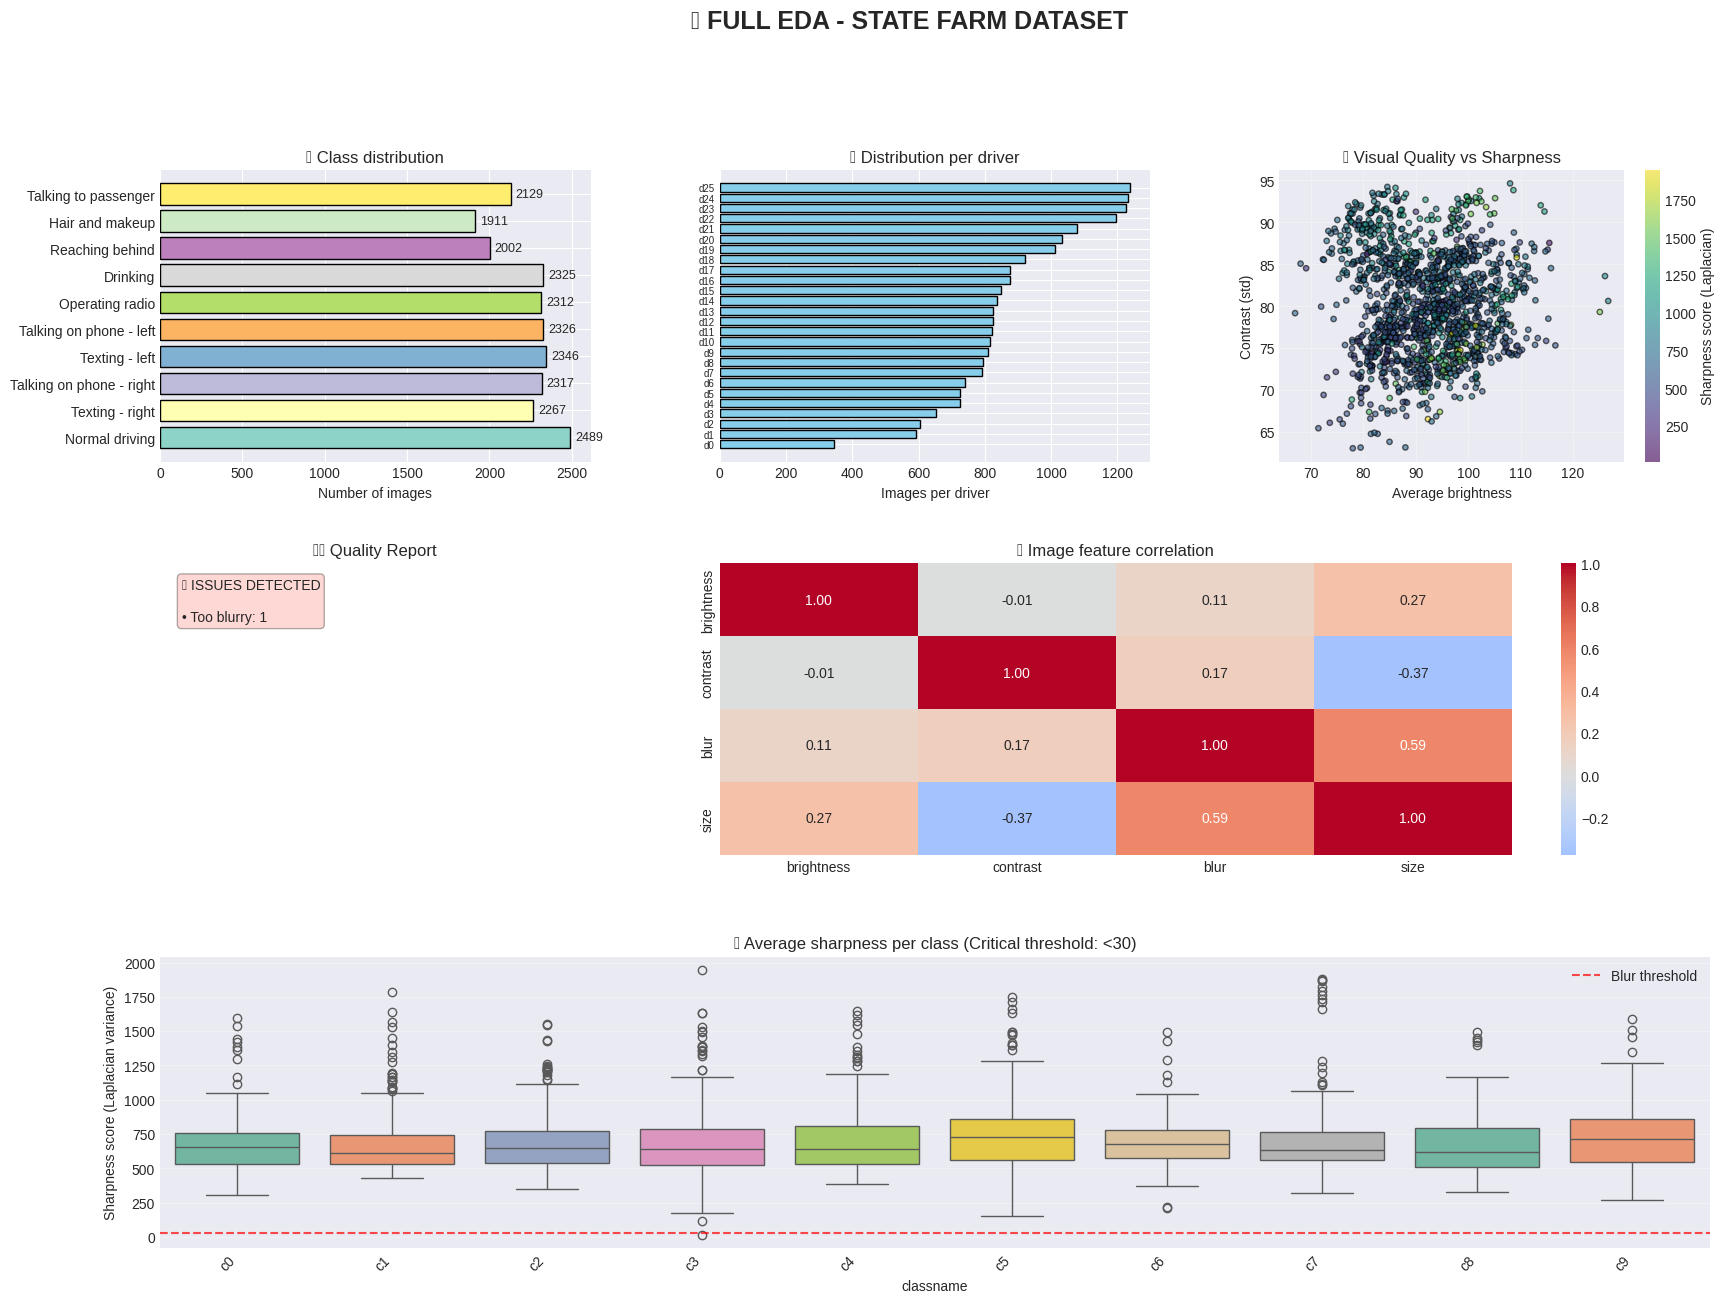
\includegraphics[width=0.98\textwidth]{1.png}
 		\caption{داشبورد جامع تحلیل اکتشافی داده‌ها (EDA) شامل توزیع کلاس‌ها، پراکندگی رانندگان، ارزیابی کیفیت بصری و همبستگی ویژگی‌های تصویر}
 		\label{fig:eda_dashboard}
 	\end{figure}
 	
 	
 	\begin{figure}[H]
 		\centering
 		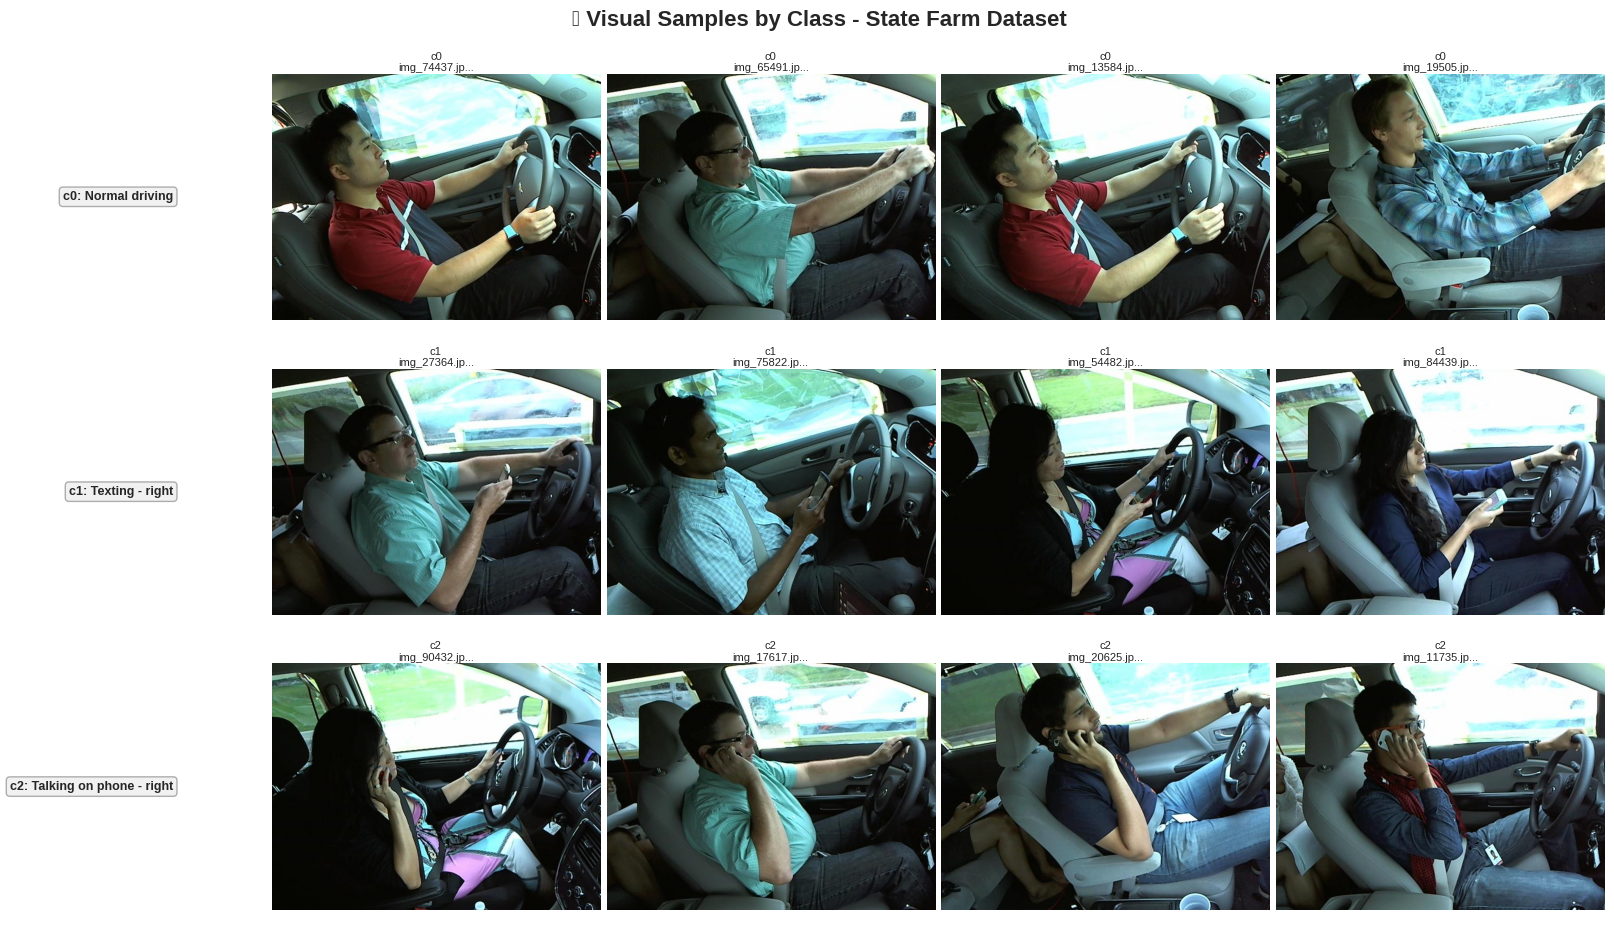
\includegraphics[width=0.98\textwidth]{3.png}
 		
 	\end{figure}
 	
 	
 	\begin{figure}[H]
 		\centering
 		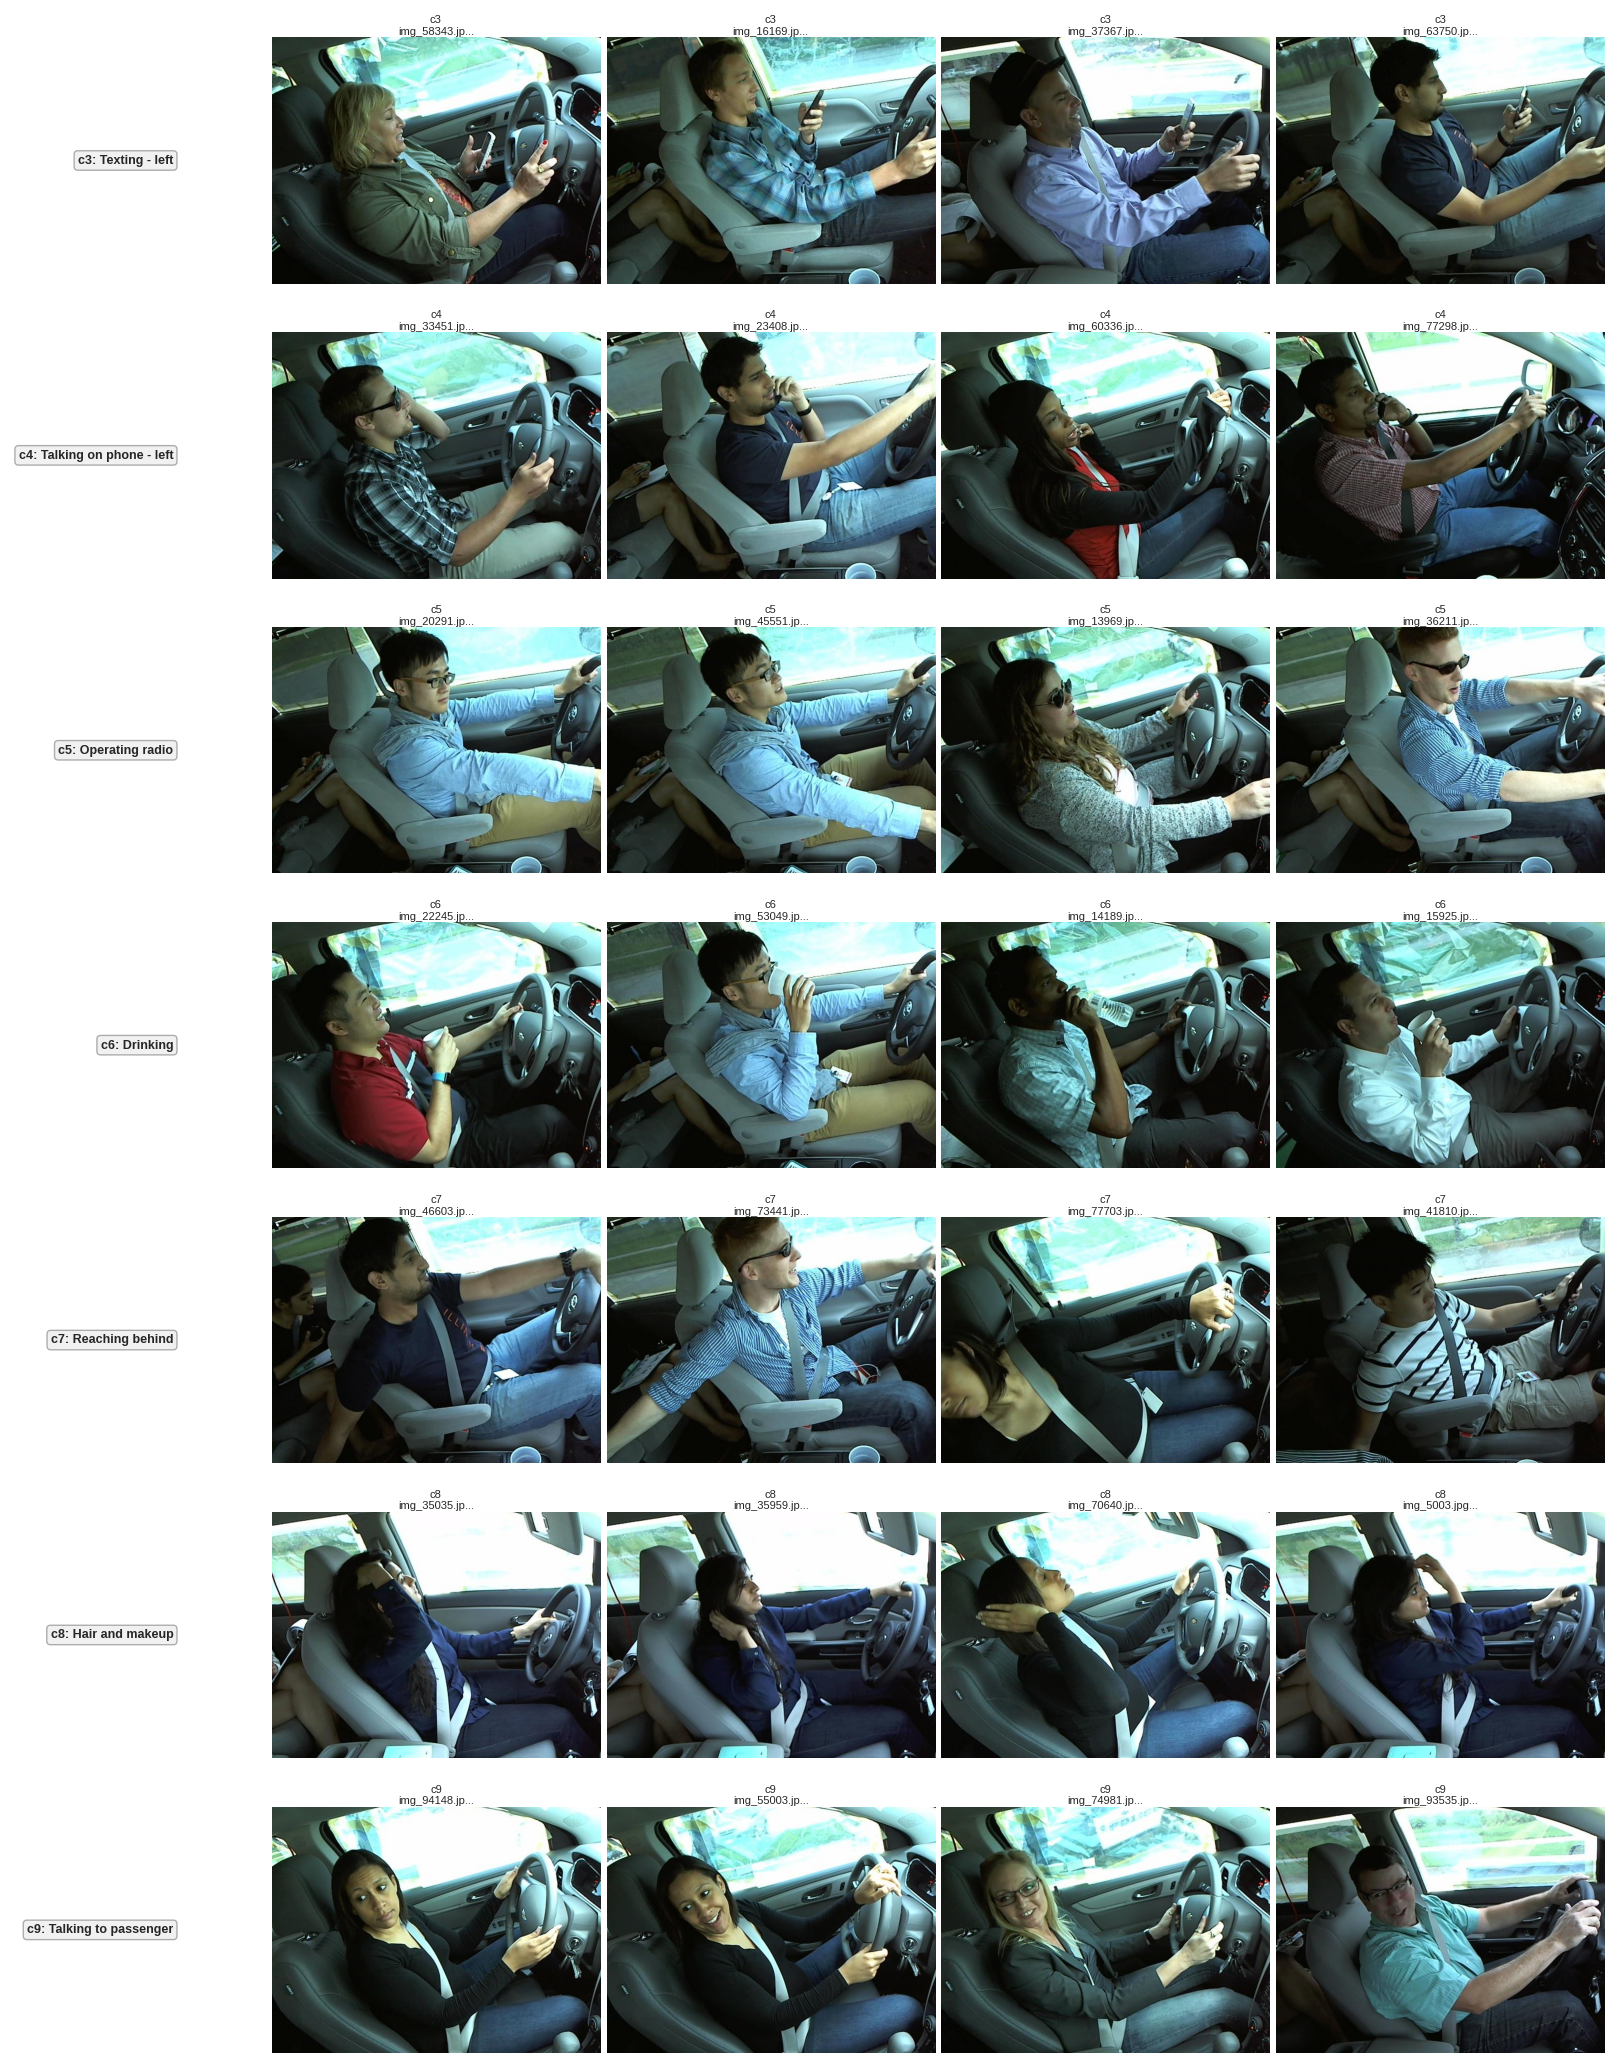
\includegraphics[width=0.98\textwidth]{2.png}
 		\caption{نمونه‌های بصری منتخب از ۱۰ حالت رفتاری راننده در مجموعه داده State Farm (۴ نمونه تصویر به ازای هر کلاس)}
 		\label{fig:class_samples_grid}
 	\end{figure}
 	
 	\begin{figure}[H]
 		\centering
 		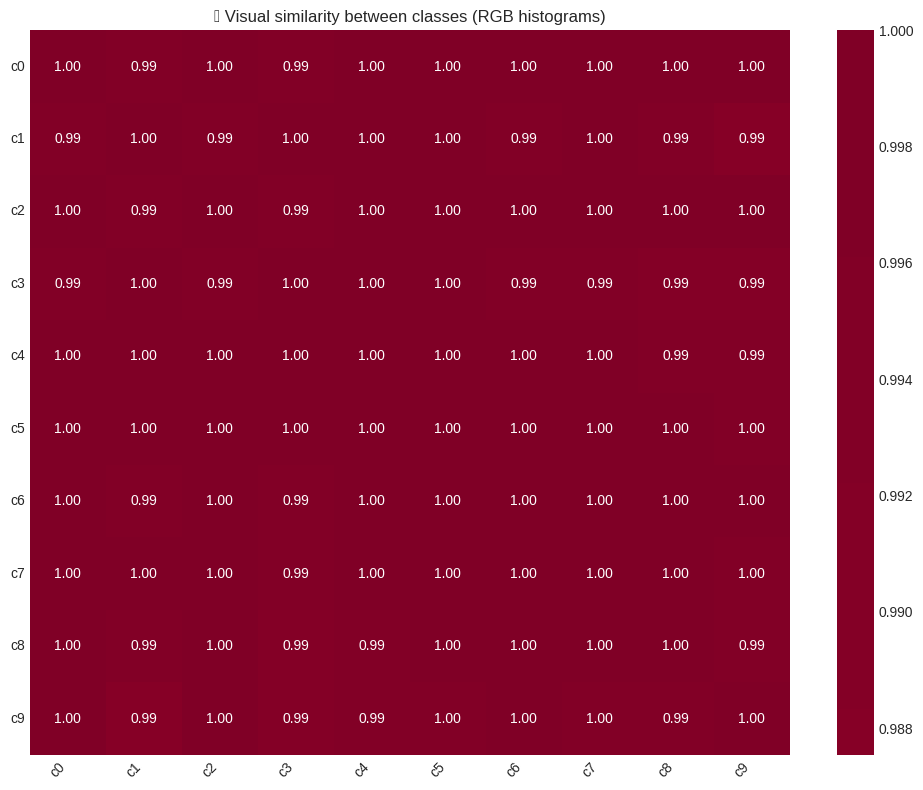
\includegraphics[width=0.75\textwidth]{4.png}
 		\caption{ماتریس شباهت بصری بین کلاس‌های ۱۰‌گانه بر اساس فاصله کسینوسی هیستوگرام‌های RGB}
 		\label{fig:class_similarity}
 	\end{figure}
 	
 	مطابق ماتریس شباهت شکل \ref{fig:class_similarity}، مقدار شباهت کسینوسی بین توزیع رنگی برخی کلاس‌ها به بالاتر از 0/95 می‌رسد. این همبستگی بالا نشان می‌دهد که تصمیم‌گیری صرف بر اساس رنگ و بافت کلی تصویر کافی نیست و شبکه باید ویژگی‌های عمیق‌تر و ساختاری دست‌ها و اشیاء را فرابگیرد.
 	
 	
 	\section{تحلیل آماری و ساختار داده‌ها}
 	مجموعه داده آموزش در این پروژه شامل مجموعاً **۲۲,۴۲۴ تصویر برچسب‌گذاری‌شده** است. برای ارزیابی دقیق و جلوگیری از تورش مدل، داده‌ها به دو بخش زیر تقسیم شده‌اند:
 	\begin{itemize}
 		\item \textbf{مجموعه آموزش ($Training Set$):} ۱۷,۹۳۹ تصویر (حدود ۸۰٪ از کل داده‌ها) برای به‌روزرسانی وزن‌های شبکه.
 		\item \textbf{مجموعه اعتبارسنجی ($Validation Set$):} ۴,۴۸۵ تصویر (حدود ۲۰٪ از کل داده‌ها) برای ارزیابی پایداری و تنظیم هایپرپارامترها.
 	\end{itemize}
 	
 	توزیع نمونه‌ها در میان کلاس‌های ۱۰‌گانه نسبتاً متوازن ($Balanced$) است که این امر مانع از غلبه یک کلاس خاص در طول فرآیند آموزش می‌شود. جدول \ref{tab:data_split} آمار دقیق تصاویر در هر کلاس را نشان می‌دهد.
 	
 	\begin{table}[H]
 		\centering
 		\caption{توزیع فراوانی تصاویر به تفکیک کلاس‌ها در مجموعه‌های آموزش و اعتبارسنجی}
 		\label{tab:data_split}
 		\small
 		\begin{tabular}{ccccc}
 			\toprule
 			\textbf{کلاس} & \textbf{شرح مختصر} & \textbf{تعداد آموزش (Train)} & \textbf{تعداد اعتبارسنجی (Val)} & \textbf{مجموع} \\
 			\midrule
 			$c0$ & رانندگی ایمن & ۱,۸۳۱ & ۴۵۸ & ۲,۲۸۹ \\
 			$c1$ & پیامک راست & ۱,۸۰۹ & ۴۵۸ & ۲,۲۶۷ \\
 			$c2$ & تلفن راست & ۱,۸۴۶ & ۴۶۱ & ۲,۳۰۷ \\
 			$c3$ & پیامک چپ & ۱,۸۷۷ & ۴۶۹ & ۲,۳۴۶ \\
 			$c4$ & تلفن چپ & ۱,۸۵. & ۴۶۲ & ۲,۳۲۶ \\
 			$c5$ & تنظیم رادیو & ۱,۸۴۹ & ۴۶۳ & ۲,۳۱۲ \\
 			$c6$ & خوردن/نوشیدن & ۱,۸۶۰ & ۴۶۵ & ۲,۳۲۵ \\
 			$c7$ & دست به عقب & ۱,۵۲۹ & ۳۸۳ & ۱,۹۱۲ \\
 			$c8$ & مو و آرایش & ۱,۵30 & ۳۸۱ & ۱,۹۱۱ \\
 			$c9$ & صحبت با سرنشین & ۱,۷۲۵ & ۴۳۱ & ۲,۱۵۶ \\
 			\midrule
 			\textbf{مجموع} & - & \textbf{۱۷,۹۳۹} & \textbf{۴,۴۸۵} & \textbf{۲۲,۴۲۴} \\
 			\bottomrule
 		\end{tabular}
 	\end{table}
 	
 	
 	
 	
 	\begin{figure}[H]
 		\centering
 		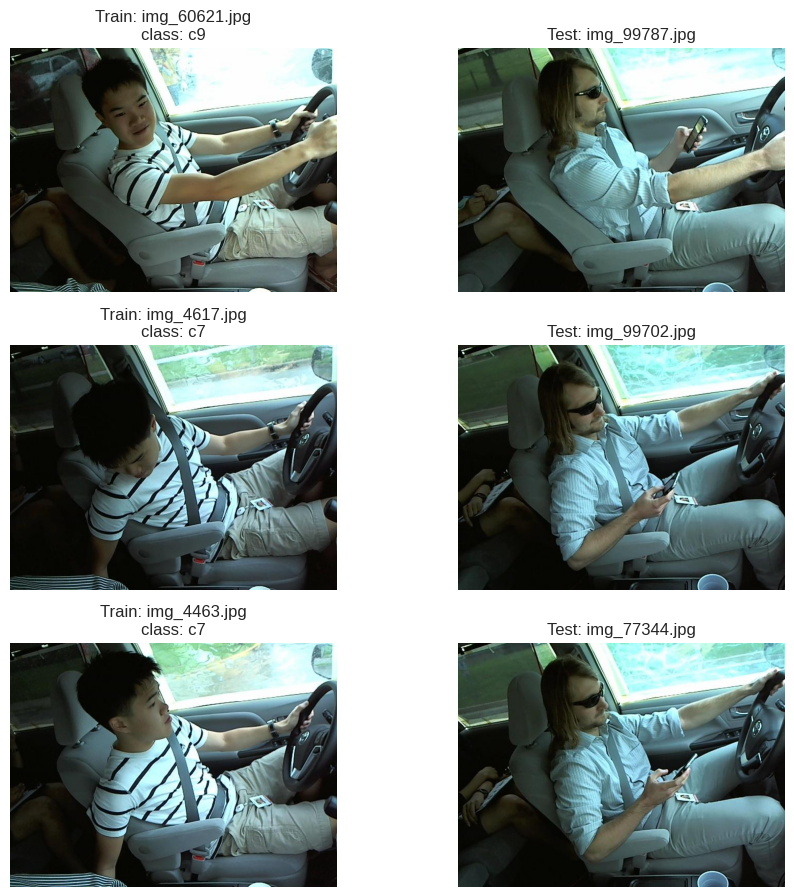
\includegraphics[width=0.92\textwidth]{18.png}
 		
 	\end{figure}
 	
 	\begin{figure}[H]
 		\centering
 		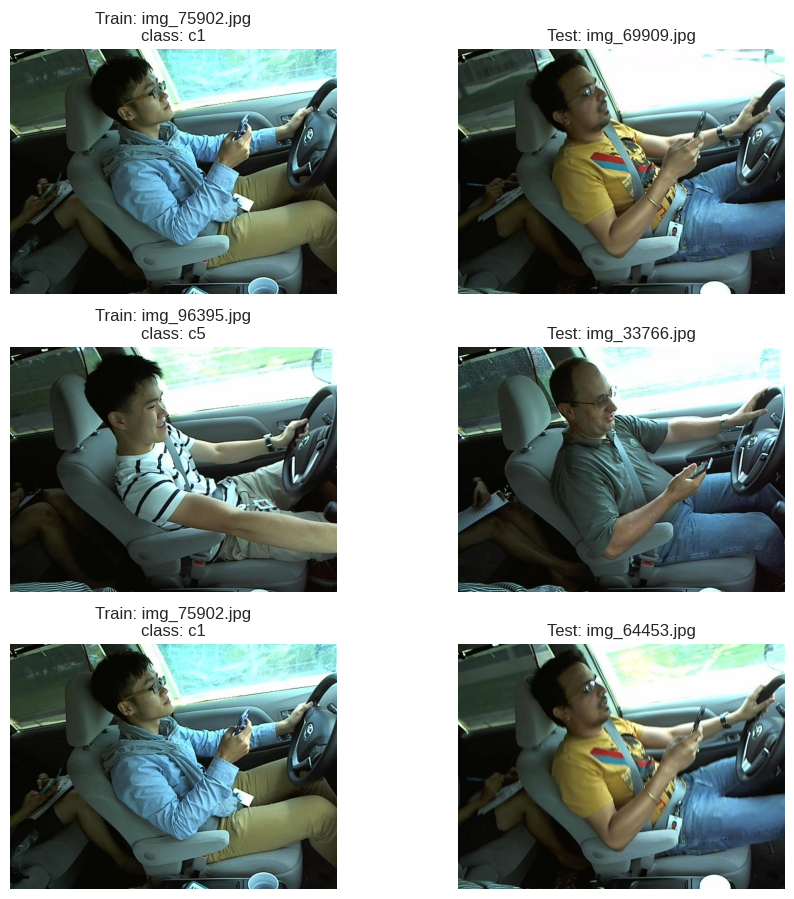
\includegraphics[width=0.92\textwidth]{17.png}
 		\caption{نمونه‌هایی از جفت‌تصاویر مشابه در مجموعه‌های آموزش (Train) و آزمون (Test) که نشان‌دهنده نشت داده‌ها (Data Leakage) در تقطیع تصادفی است.}
 		\label{fig:train_test_leakage}
 	\end{figure}
 	
 	
 	
 	یکی از چالش‌های بنیادین در مجموعه‌داده \lr{State Farm Distracted Driver Detection}، حضور یک راننده مشخص در چندین فریم پیاپی است. در صورتی که تقسیم‌بندی داده‌ها به صورت کاملاً تصادفی انجام شود، تصاویری از یک راننده واحد هم در مجموعه آموزش و هم در مجموعه اعتبارسنجی/آزمون قرار می‌گیرند (شکل \ref{fig:train_test_leakage}). 
 	
 	این پدیده که تحت عنوان نشت داده‌ها (\lr{Data Leakage}) شناخته می‌شود، سبب می‌گردد مدل به جای یادگیری «ویژگی‌های انتزاعی رفتار رانندگی»، «ویژگی‌های دیداری خاص آن راننده» (مانند رنگ لباس، پس‌زمینه خودرو یا زاویه صندلی) را به خاطر بسپارد. این امر منجر به ارزیابی بیش از حد خوش‌بینانه و کاذب در مرحله اعتبارسنجی می‌شود. جهت رفع این چالش در فرایند پیاده‌سازی، تقطیع داده‌ها بر اساس شناسه رانندگان (\lr{Driver ID}) و با استفاده از روش \lr{GroupKFold} انجام شده است تا ارزیابی مدل کاملاً مستقل از هویت رانندگان صورت پذیرد.
 	
 	
 	
 	
 	
 	\section{تکنیک‌های افزایش داده (Data\_Augmentation)}
 	یکی از چالش‌های اصلی در آموزش شبکه‌های عمیق، خطر بیش‌برازش ($Overfitting$) رو داده‌های آموزشی است. برای بهبود قدرت تعمیم‌پذیری ($Generalization$) مدل بر روی تصاویر جدید، از الگوریتم‌های افزایش خطی و هندسی داده‌ها در طول بارگذاری استفاده شده است.
 	
 	\subsection{تغییرات هندسی و رنگی}
 	عملیات ریاضی اعمال‌شده بر روی تصاویر ورودی شامل موارد زیر است:
 	
 	\begin{enumerate}
 		\item \textbf{چرخش تصادفی (Random\_Rotation)}: اعمال دوران حول مرکز تصویر با زاویه $\theta \in [-10^\circ, +10^\circ]$. ماتریس دوران دوبعدی عبارت است از:
 		\begin{equation}
 			\begin{bmatrix} x' \\ y' \end{bmatrix} = \begin{bmatrix} \cos\theta & -\sin\theta \\ \sin\theta & \cos\theta \end{bmatrix} \begin{bmatrix} x - x_c \\ y - y_c \end{bmatrix} + \begin{bmatrix} x_c \\ y_c \end{bmatrix}
 		\end{equation}
 		
 		\item \textbf{انتقال افقی و عمودی (Random\_Translation)}: جابه‌جایی پیکسل‌ها به اندازه $t_x, t_y$ تا حداکثر ۱۰٪ ابعاد تصویر:
 		\begin{equation}
 			I_{new}(x, y) = I(x - t_x, y - t_y)
 		\end{equation}
 		
 		\item \textbf{تغییر مقیاس تصادفی (Random\_Zoom)}: بزرگ‌نمایی یا کوچک‌نمایی تصویر با ضریب $s \in [0.9, 1.1]$.
 	\end{enumerate}
 	
 	\begin{quote}
 		\textbf{نکته طراحی مهندسی:} به دلیل حیاتی بودن موقعیت دست‌ها (دست راست یا چپ بودن تلفن/پیامک)، از **بازتاب افقی (Horizontal\_Flip)** استفاده نشده است؛ زیرا بازتاب افقی کلاس $c1$ (پیامک با دست راست) را فرآیندی مشابه $c3$ (پیامک با دست چپ) تغییر می‌دهد و الگوریتم را دچار سردرگمی می‌کند.
 	\end{quote}
 	
 	
 	
 	
 	\begin{figure}[H]
 		\centering
 		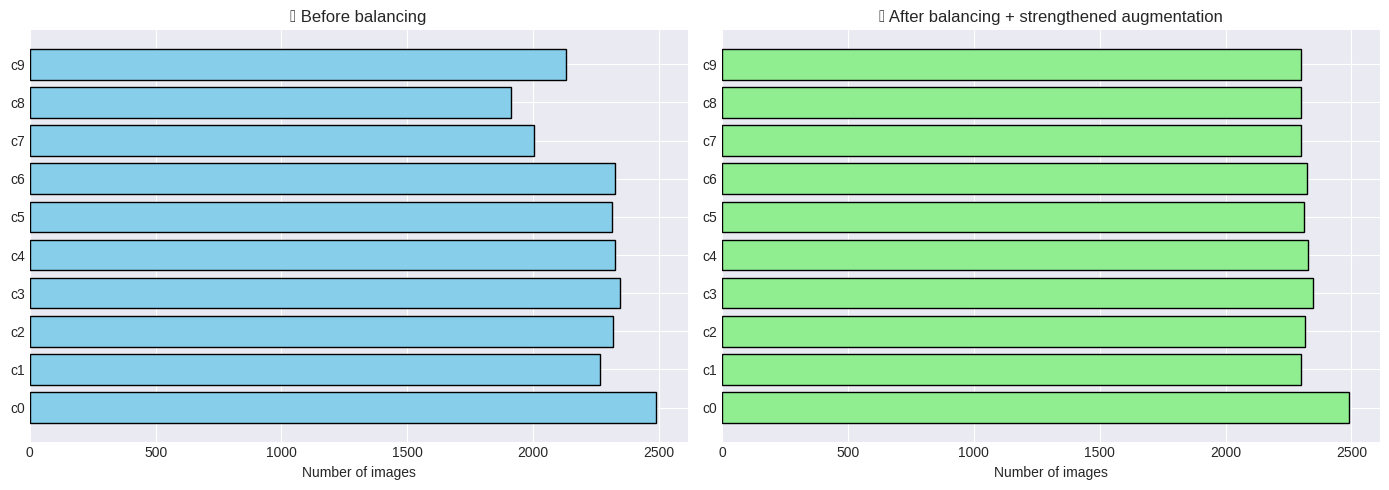
\includegraphics[width=0.95\textwidth]{5.png}
 		\caption{مقایسه توزیع فراوانی تصاویر کلاس‌های ۱۰‌گانه پیش از متوازن‌سازی و پس از اعمال افزون‌سازی تقویت‌شده (رساندن تمام کلاس‌ها به ۲۳۰۰ نمونه)}
 		\label{fig:balancing_comparison}
 	\end{figure}
 	
 	همان‌طور که در شکل \ref{fig:balancing_comparison} (سمت چپ) مشاهده می‌شود، ناهمگونی و عدم توازن اولیه در تعداد نمونه‌های کلاس‌های مختلف وجود داشت که می‌توانست موجب سوگیری مدل به سمت کلاس‌های اکثر شود. جهت رفع این چالش، استراتژی متوازن‌سازی هوشمند با اعمال تغییرات هندسی و نوری تقویت‌شده (\lr{Strengthened Augmentation}) پیاده‌سازی گردید.پارامترهای افزون‌سازی به گونه‌ای تنظیم شدند که ضمن افزایش تنوع داده‌ها، ویژگی‌های حیاتی حفظ شوند. به عنوان مثال، پارامتر چرخش افقی (\lr{Horizontal Flip}) به صورت دقیق غیرفعال (\lr{False}) نگه داشته شد؛ زیرا تغییر جهت دست راننده (راست‌دست یا چپ‌دست بودن) ماهیت معنایی کلاس‌ها (مانند تفاوت $c_1$ و $c_3$) را تغییر می‌دهد. در نهایت، با تولید نمونه‌های سنتیز شده، تمام کلاس‌ها دقیقاً روی تعداد ۲,۳۰۰ تصویر متوازن گردیدند (شکل \ref{fig:balancing_comparison} سمت راست).
 	
 	
 	
 	\begin{figure}[H]
 		\centering
 		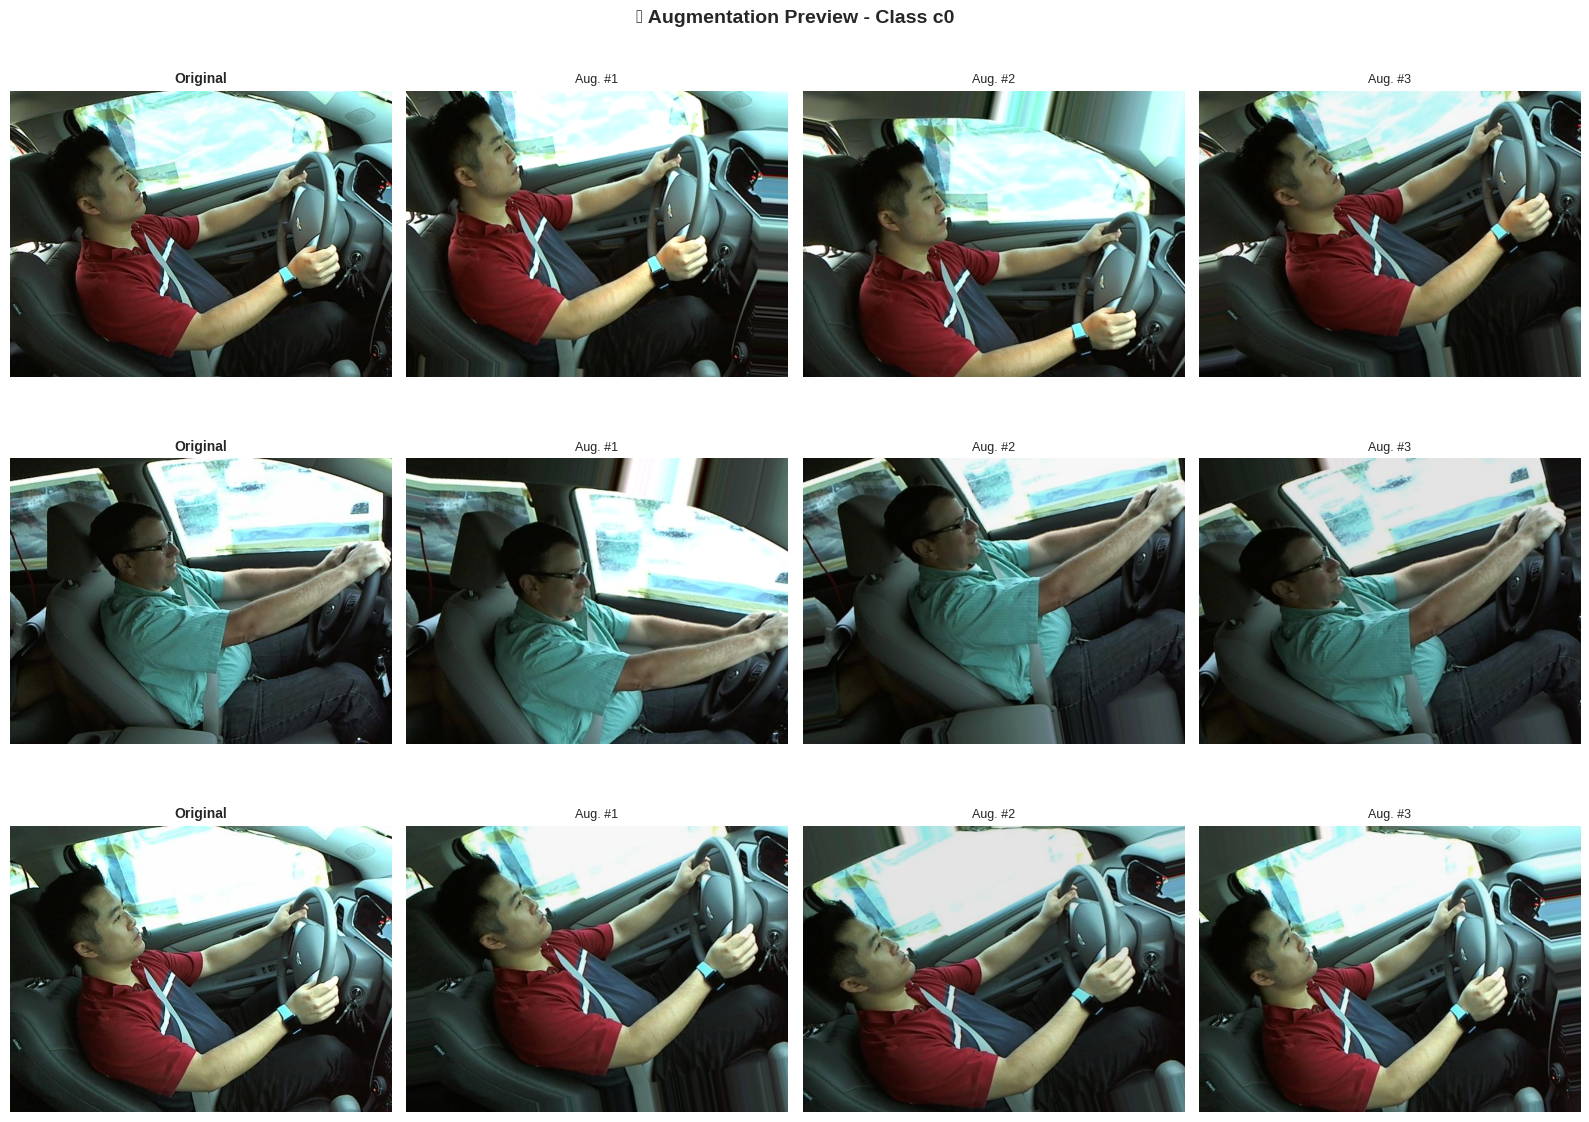
\includegraphics[width=0.95\textwidth]{6.png}
 		\caption{پیش‌نمایش افزون‌سازی برای کلاس $c_0$ (رانندگی عادی)}
 		\label{fig:aug_c0}
 	\end{figure}
 	
 	
 	\begin{figure}[H]
 		\centering
 		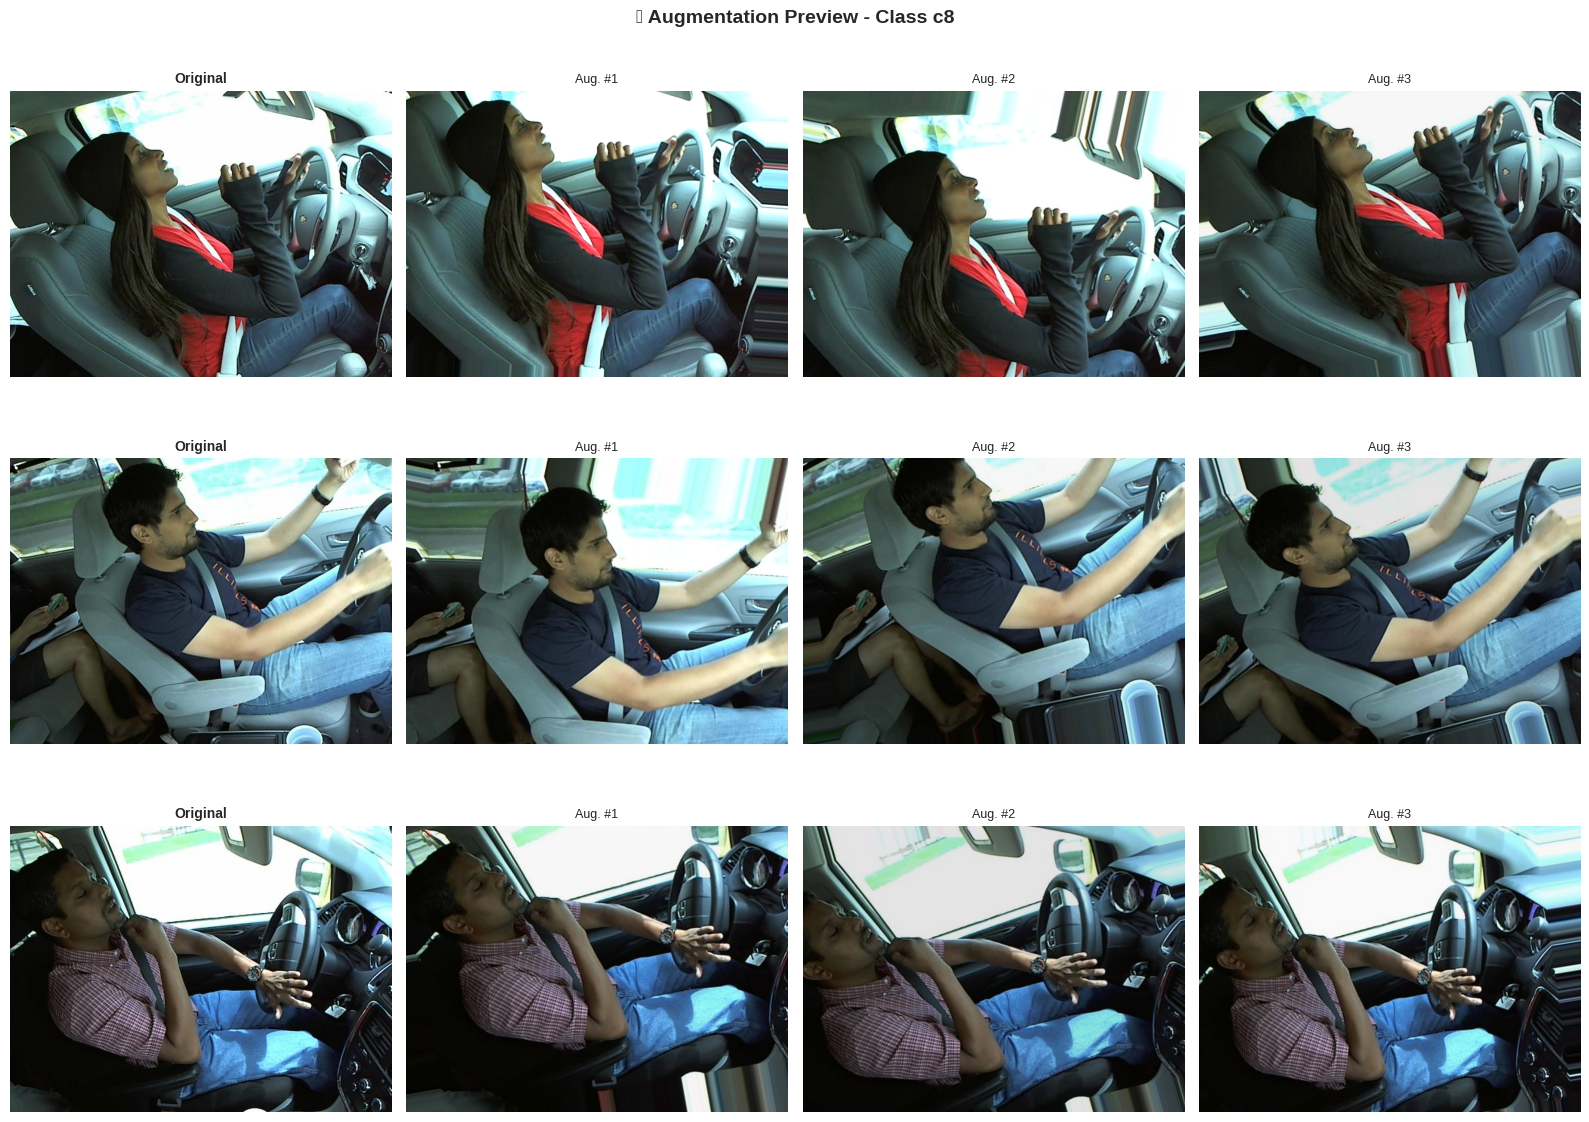
\includegraphics[width=0.95\textwidth]{7.png}
 		\caption{پیش‌نمایش افزون‌سازی برای کلاس $c_8$ (مرتب‌کردن مو/آرایش)}
 		\label{fig:aug_c8}
 	\end{figure}
 	
 	
 	
 	جهت اطمینان از حفظ ماهیت معنایی تصاویر پس از اعمال دگرگونی‌ها، پیش‌نمایش تغییرات برای نمونه‌هایی از کلاس‌های مختلف (شکل \ref{fig:aug_c0} و \ref{fig:aug_c8}) مورد بررسی قرار گرفت.
 	
 	مطابق تصاویر خروجی:
 	\begin{itemize}
 		\item تغییرات نوری و جابه‌جایی‌های جزئی (\lr{Shift \& Brightness Adjustment}) شرایط واقعی متغیر بودن نور داخل کابین خودرو و زوایای مختلف دوربین را به‌خوبی شبیه‌سازی می‌کنند.
 		\item هندسه اصلی راننده و ابزارهای در دست او (مانند تلفن همراه یا لیوان) تحت تأثیر جابه‌جایی‌ها تخریب نشده و ساختار کلاس کاملاً محفوظ مانده است.
 	\end{itemize}
 	
 	
 	
 	
 	
 	\section{تغییر ابعاد و نرمال‌سازی تصاویر ورودی}
 	
 	\subsection{تغییر مقیاس فضایی (Resizing)}
 	تصاویر اصلی با ابعاد $640 \times 480 \times 3$ جهت کاهش بار محاسباتی و تطابق با استاندارد شبکه به ابعاد زیر تغییر می‌یابند:
 	\begin{equation}
 		I_{input} \in \mathbb{R}^{224 \times 224 \times 3}
 	\end{equation}
 	
 	\subsection{پیش‌پردازش و نرمال‌سازی اختصاصی مدل‌ها}
 	شبکه‌های پیش‌آموزش‌دیده بر روی $ImageNet$ نیازمند نرمال‌سازی دقیق پیکسل‌ها مطابق با فرآیند اولیه آموزش خود هستند. در این پروژه دو خط‌لوله پیش‌پردازش متفاوت پیاده‌سازی گردید:
 	
 	\subsubsection{۱. پیش‌پردازش در شبکه MobileNetV2}
 	پیکسل‌های تصویر ورودی که در ابتدا در دامنه $[0, 255]$ قرار دارند، با استفاده از تابع پیش‌پردازش استاندارد $MobileNet$ به دامنه $[-1, 1]$ نگاشت می‌شوند:
 	\begin{equation}
 		x_{norm} = \frac{x}{127.5} - 1.0 \quad \implies \quad x_{norm} \in [-1.0, 1.0]
 	\end{equation}
 	
 	\subsubsection{۲. پیش‌پردازش در شبکه ResNet50}
 	در پیاده‌سازی ارائه شده برای $ResNet50$، لایه پیش‌پردازش اختصاصی `preprocess\_input` مستقیماً در انتهای خط‌ لوله ورودی قرار داده شد. این تابع، کانال‌های رنگی را از $RGB$ به $BGR$ تبدیل کرده و میانگین شدت روشنایی کانال‌های پایگاه داده $ImageNet$ را از آن‌ها کسر می‌کند:
 	\begin{equation}
 		\begin{cases}
 			B' = B - 103.939 \\
 			G' = G - 116.779 \\
 			R' = R - 123.680
 		\end{cases}
 	\end{equation}
 	همچنین مقادیر شدت پیکسل ورودی در دامنه $[0, 1]$ وارد این لایه اختصاصی می‌گردند.
 	
 	
 	
 	\begin{figure}[H]
 		\centering
 		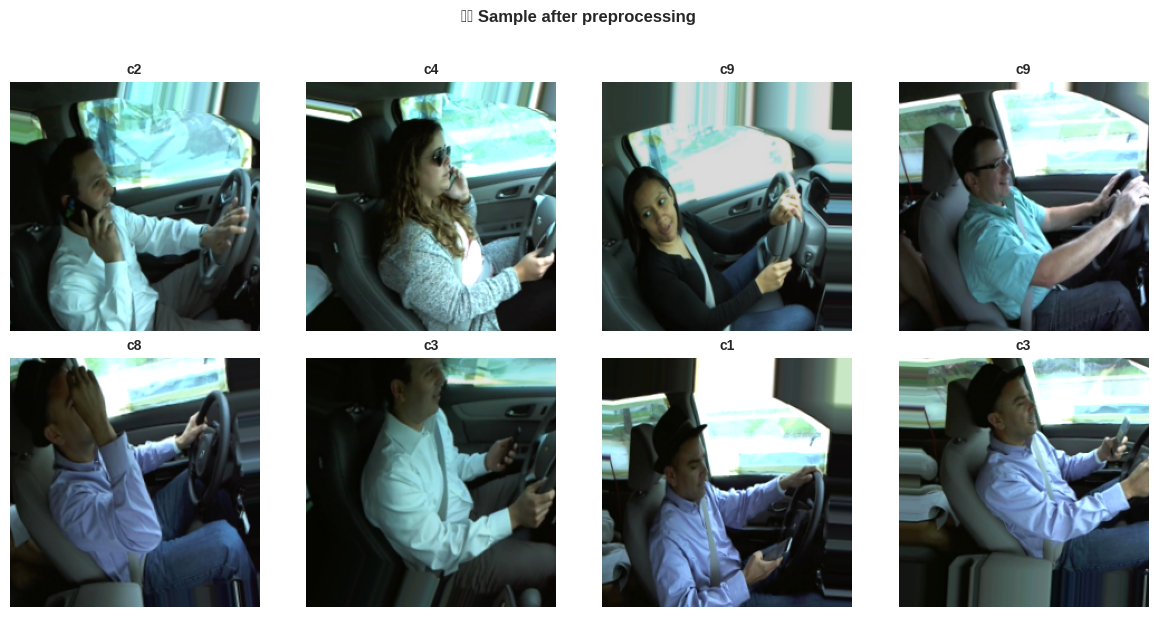
\includegraphics[width=0.88\textwidth]{8.png}
 		\caption{نمونه‌ای از داده‌های ورودی آماده‌شده پس از طی مراحل خط‌لوله پیش‌پردازش (تغییر سایز به $224 \times 224$، نرمال‌سازی دامنه پیکسل‌ها به $[0, 1]$ و اعمال الگوریتم‌های افزون‌سازی)}
 		\label{fig:preprocessing_sample}
 	\end{figure}
 	
 	جهت اطمینان از صحت عملکرد ژنراتورهای داده (\lr{ImageDataGenerator}) و آماده‌سازی بسته‌های ورودی (\lr{Batches}) برای شبکه‌های عمیق، نمونه‌ای از خروجی خط‌لوله در شکل \ref{fig:preprocessing_sample} نمایش داده شده است.همان‌طور که مشخص است، تمامی تصاویر به رزولوشن ورودی استاندارد $224 \times 224 \times 3$ تبدیل شده، دامنه‌ی بازه مقادیر پیکسل‌ها از $[0, 255]$ به $[0, 1]$ نگاشت یافته و برچسب‌های مربوط به هر کلاس به‌صورت ماتریس‌های  \lr{One-Hot Encoding} تنظیم شده‌اند. این گام، آخرین مرحله از فاز پیش‌پردازش بوده و بستر داده‌ها را برای ورود به مرحله آموزش شبکه‌های \lr{ResNet50} و \lr{MobileNetV2} آماده می‌سازد.
 	
 	\section{جمع‌بندی فصل}
 	در این فصل ویژگی‌های آمارشناسی مجموعه داده State\_Farm، کلاس‌های ۱۰‌گانه و نحوه تقسیم داده‌ها بررسی شد. همچنین اهمیت عدم استفاده از Horizontal\_Flip برای حفظ یکپارچگی برچسب‌های دست چپ/راست تحلیل گردید و معادلات نرمال‌سازی ورودی برای هر دو شبکه MobileNetV2 و ResNet50 تثبیت شد. این پیش‌پردازش‌های دقیق، زیرساخت ورود داده‌ها به فاز آموزش مدل‌ها در فصل بعدی را تشکیل می‌دهند.
 	
 	
 	
 	
 	
 	
 	
 	\chapter{معماری پیشنهادی و روش‌شناسی}
 	
 	\section{مقدمه}
 	پس از تحلیل پایگاه داده و انجام پیش‌پردازش‌های لازم، در این فصل جزئیات معماری‌های پیاده‌سازی‌شده و خط‌لوله (Pipeline) آموزش شبکه‌ها تشریح می‌گردد. رویکرد اصلی این پژوهش، بهره‌گیری از \textbf{یادگیری انتقالی (Transfer\_Learning)} مبتنی بر وزن‌های پیش‌آموزش‌دیده بر روی مجموعه داده عظیم ImageNet است.
 	
 	در ادامه، جزئیات لایه‌های سفارشی افزوده‌شده به بدنه اصلی شبکه‌ها، استراتژی آموزش دو فازی (شامل فاز استخراج ویژگی و فاز تنظیم دقیق)، تنظیم هایپرپارامترها و مکانیزم‌های کنترلی آموزش مورد تحلیل دقیق قرار می‌گیرند.
 	
 	\section{معماری شبکه و لایه‌های سفارشی (Custom\_Classification\_Head)}
 	برای انطباق وزن‌های پیش‌آموزش‌دیده شبکه‌های ResNet50 و MobileNetV2 با مسئله ۱۰ کلاسه تشخیص حواس‌پرتی راننده، لایه‌های انتهای (Dense\_Head) این شبکه‌ها حذف گردیده و یک سر طبقه‌بندی سفارشی عمیق بر روی آن‌ها جای‌گذاری شده است.
 	
 	\subsection{ساختار لایه‌های سفارشی}
 	سر طبقه‌بندی طراحی‌شده شامل لایه‌های زیر به ترتیب است:
 	\begin{enumerate}
 		\item \textbf{لایه Global\_Average\_Pooling\_2D\_(GAP)}: کاهش ابعاد فضایی نقشه ویژگی‌های خروجی از بدنه اصلی به یک بردار یک‌بعدی.
 		\item \textbf{لایه Fully\_Connected اول (Dense)}: شامل ۵۱۲ نورون با تابع فعال‌سازی $ReLU$ جهت استخراج نگاشت‌های انتزاعی سطح بالا.
 		\item \textbf{لایه Dropout اول:} با نرخ $0.5$ جهت حذف تصادفی اتصالات در طول آموزش و جلوگیری از بیش‌برازش ($Overfitting$).
 		\item \textbf{لایه Fully\_Connected دوم (Dense)}: شامل ۲۵۶ نورون با تابع فعال‌سازی $ReLU$ برای فشرده‌سازی بیشتر ویژگی‌ها.
 		\item \textbf{لایه Dropout دوم:} با نرخ $0.3$ جهت تثبیت بیشتر پایداری شبکه.
 		\item \textbf{لایه خروجی (Dense\_Output\_Layer)}: شامل ۱۰ نورون با تابع فعال‌سازی $Softmax$ جهت تولید توزیع احتمالی پیش‌بینی‌ها برای ۱۰ کلاس رفتار راننده.
 	\end{enumerate}
 	
 	جدول \ref{tab:model_head_structure} خلاصه ساختار لایه‌های سفارشی متصل‌شده به انتهای هر دو بدنه اصلی را نشان می‌دهد.
 	
 	\begin{table}[H]
 		\centering
 		\caption{ساختار لایه‌های سفارشی سر طبقه‌بندی (Custom\_Classification\_Head)}
 		\label{tab:model_head_structure}
 		\small
 		\begin{tabular}{cccc}
 			\toprule
 			\textbf{نام لایه} & \textbf{نوع لایه} & \textbf{ابعاد خروجی / تعداد نورون} & \textbf{تابع فعال‌سازی / پارامتر} \\
 			\midrule
 			\lr{Base Model Output} & - & $H \times W \times C$ & - \\
 			\lr{GlobalAvgPooling2D} & Pooling & $C$ & - \\
 			\lr{Dense 1} & Fully Connected & 512 & ReLU \\
 			\lr{Dropout 1} & Regularization & 512 & Rate = 0/5 \\
 			\lr{Dense 2} & Fully Connected & 256 & ReLU \\
 			\lr{Dropout 2} & Regularization & 256 & Rate = 0/3 \\
 			\lr{Output Dense} & Fully Connected & 10 & Softmax \\
 			\bottomrule
 		\end{tabular}
 	\end{table}
 	
 	
 	
 	
 	
 	
 	
 	
 	
 	\subsection{معماری شبکه پیشنهادی مبتنی بر MobileNetV2}
 	\label{sec:mobilenetv2_arch}
 	
 	جهت استخراج ویژگی‌های کلیدی از تصاویر رانندگان، از شبکه پیش‌آموخته \lr{MobileNetV2} به عنوان بدنه اصلی (\lr{Backbone}) استفاده گردید. لایه‌های سر طبقه‌بندی‌کننده (\lr{Classification Head}) جدیدی به انتهای این شبکه اضافه شدند. نمودار بلاکی ساختار دقیق لایه‌ها و جریان داده‌ها در شکل \ref{fig:mobilenetv2_arch} نشان داده شده است.
 	
 	\begin{figure}[H]
 		\centering
 		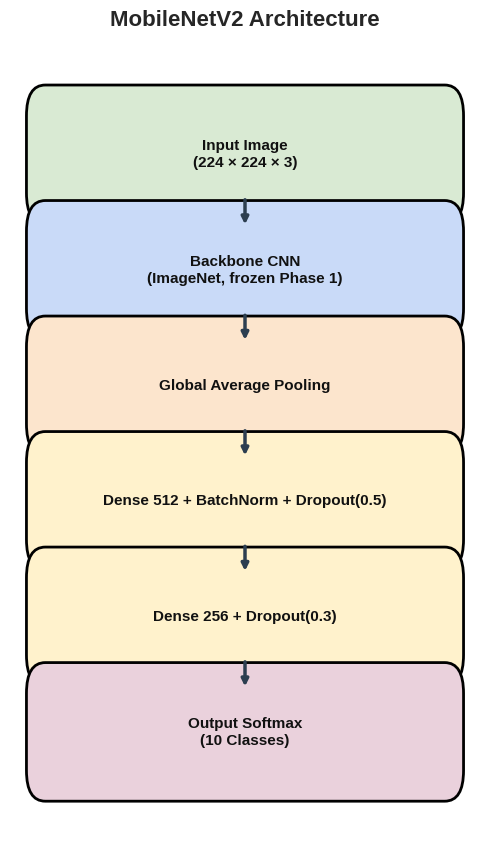
\includegraphics[width=0.55\textwidth]{29.png}
 		\caption{نمودار بلوکی معماری شبکه پیشنهادی مبتنی بر MobileNetV2.}
 		\label{fig:mobilenetv2_arch}
 	\end{figure}
 	
 	همان‌طور که در شکل \ref{fig:mobilenetv2_arch} مشخص است، تصاویر ورودی با ابعاد $224 \times 224 \times 3$ وارد شبکه شده و پس از گذر از لایه‌های استخراج ویژگی، توسط لایه \lr{Global Average Pooling} خلاصه می‌شوند. سپس دو لایه کامل متصل (\lr{Dense}) به همراه لایه‌های \lr{Dropout} (با نرخ‌های ۰.۵ و ۰.۳) و \lr{Batch Normalization} جهت جلوگیری از بیش‌برازش قرار گرفته‌اند.
 	
 	
 	
 	
 	
 	
 	\subsection{معماری شبکه پیشنهادی مبتنی بر ResNet50}
 	\label{sec:resnet50_arch}
 	
 	معماری دوم بر پایه شبکه عمیق \lr{ResNet50} طراحی شده است. ساختار لایه‌های افزوده‌شده کاملاً مشابه مدل قبل تنظیم گردید تا امکان مقایسه عادلانه فراهم شود. دیاگرام ساختار این شبکه در شکل \ref{fig:resnet50_arch} به تصویر کشیده شده است.
 	
 	\begin{figure}[H]
 		\centering
 		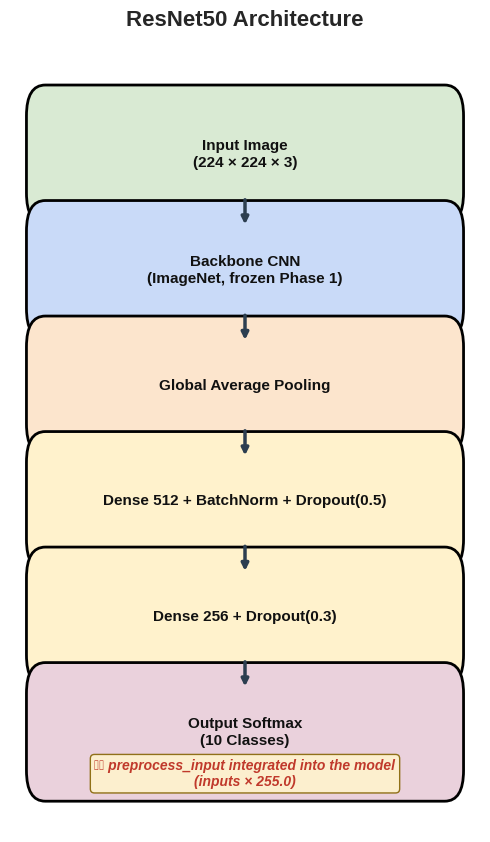
\includegraphics[width=0.55\textwidth]{30.png}
 		\caption{نمودار بلوکی معماری شبکه پیشنهادی مبتنی بر ResNet50 به همراه لایه پیش‌پردازش یکپارچه.}
 		\label{fig:resnet50_arch}
 	\end{figure}
 	
 	نکته حائز اهمیت در معماری شکل \ref{fig:resnet50_arch}، ادغام مستقیم تابع پیش‌پردازش (\lr{preprocess\_input}) در ورودی مدل است؛ بدین صورت که تصاویر نرمال‌شده در بازه $[0, 1]$ پس از ورود به مدل، به صورت داخلی در عدد ۲۵۵ ضرب شده و آماده ورود به بلوک‌های باقی‌مانده (\lr{Residual Blocks}) می‌گردند.
 	
 	
 	
 	
 	
 	
 	
 	
 	
 	
 	
 	\section{استراتژی آموزش دو فازی (Two-Phase\_Training\_Strategy)}
 	برای دستیابی به بیشترین دقت اعتبارسنجی و همگرایی پایدار، فرآیند آموزش شبکه‌ها به دو فاز مجزا تقسیم شده است.
 	
 	\subsection{فاز اول: استخراج ویژگی (Feature\_Extraction)}
 	در این فاز، تمام لایه‌های بدنه اصلی شبکه (Backbone) منجمد ($Frozen$) می‌شوند. هدف اصلی این فاز، آموزش اولیه لایه‌های سفارشی جدید بدون دست‌کاری و تخریب وزن‌های ارزشمند پیش‌آموزش‌دیده ImageNet است.
 	\begin{itemize}
 		\item \textbf{وضعیت لایه‌ها:} \lr{Base Model Layers = Non-trainable}
 		\item \textbf{پارامترهای قابل آموزش:} فقط پارامترهای سر طبقه‌بندی سفارشی.
 		\item \textbf{نرخ یادگیری (Learning\_Rate)}: نرخ نسبتاً بالای $\eta_1 = 10^{-3}$ جهت همگرایی سریع لایه‌های جدید.
 		\item \textbf{تعداد دوره‌ها (Epochs)}: آموزش به مدت ۱۰ تا ۱۵ دور اولیه.
 	\end{itemize}
 	
 	\subsection{فاز دوم: تنظیم دقیق (Fine-Tuning)}
 	پس از همگرایی اولیه سر طبقه‌بندی، قفل لایه‌های عمیق بدنه اصلی باز می‌شود ($Unfrozen$) تا لایه‌های فوقانی شبکه بتوانند ویژگی‌های بصری خود را متناسب با جزئیات خاص مجموعه داده State\_Farm (مانند وضعیت دقیق انگشتان یا زاویه دید داخل کابین) تطبیق دهند.
 	\begin{itemize}
 		\item \textbf{وضعیت لایه‌ها در ResNet50}: آزادسازی لایه‌های بلاک انتهای شبکه (حدود ۳۰ لایه آخری) برای تنظیم دقیق.
 		\item \textbf{وضعیت لایه‌ها در MobileNetV2}: آزادسازی لایه‌های فوقانی (از لایه ۱۰۰ به بعد).
 		\item \textbf{نرخ یادگیری (Learning\_Rate)}: استفاده از نرخ یادگیری بسیار کوچک $\eta_2 = 10^{-5}$ جهت جلوگیری از تغییرات شدید و مخرب در وزن‌های پیش‌آموزش‌دیده.
 		\item \textbf{تعداد دوره‌ها (Epochs)}: ادامه آموزش به مدت ۱۵ تا ۲۰ دوره تکمیلی.
 	\end{itemize}
 	
 	\section{هایپرپارامترها و مکانیزم‌های کنترلی آموزش}
 	
 	\subsection{تنظیمات هایپرپارامترها}
 	جدول \ref{tab:hyperparameters} هایپرپارامترهای کلیدی مورد استفاده در آموزش هر دو شبکه را نشان می‌دهد.
 	
 	\begin{table}[H]
 		\centering
 		\caption{تنظیمات هایپرپارامترهای آموزش شبکه‌ها}
 		\label{tab:hyperparameters}
 		\small
 		\begin{tabular}{ccc}
 			\toprule
 			\textbf{هایپرپارامتر} & \textbf{مقدار در فاز ۱ (Feature\_Extraction)} & \textbf{مقدار در فاز ۲ (Fine-Tuning)} \\
 			\midrule
 			اندازه دسته (\lr{Batch Size}) & 32 & 32 \\
 			بهینه‌ساز (\lr{Optimizer}) & Adam ($\beta_1=0.9, \beta_2=0.999$) & Adam ($\beta_1=0.9, \beta_2=0.999$) \\
 			نرخ یادگیری (\lr{Learning Rate}) & $1 \times 10^{-3}$ & $1 \times 10^{-5}$ \\
 			تابع زیان (\lr{Loss Function}) & Categorical Cross-Entropy & Categorical Cross-Entropy \\
 			معیار اصلی (\lr{Metric}) & Accuracy & Accuracy \\
 			\bottomrule
 		\end{tabular}
 	\end{table}
 	
 	\subsection{کال‌بک‌ها و مکانیزم‌های کنترلی (Callbacks)}
 	برای نظارت بر روند آموزش و جلوگیری از بیش‌برازش، از سه مکانیزم هوشمند استفاده گردید:
 	\begin{enumerate}
 		\item \textbf{کال‌بک `ModelCheckpoint`}: ذخیره خودکار بهترین وزن‌های شبکه بر اساس کمترین میزان زیان اعتبارسنجی ($val\_loss$).
 		\item \textbf{کال‌بک `ReduceLROnPlateau`}: کاهش خودکار نرخ یادگیری با ضریب $0.2$ در صورتی که زیان اعتبارسنجی به مدت ۳ دوره پیاپی بهبودی پیدا نکند ($factor=0.2, patience=3$).
 		\item \textbf{کال‌بک `EarlyStopping`}: متوقف کردن فرآیند آموزش در صورت عدم بهبود عملکرد اعتبارسنجی به مدت ۵ دوره پیاپی ($patience=5$) جهت جلوگیری از اتلاف منابع محاسباتی.
 	\end{enumerate}
 	
 	\section{جمع‌بندی فصل}
 	در این فصل معماری لایه‌های طبقه‌بندی سفارشی، دلایل استفاده از لایه‌های GAP و Dropout و استراتژی آموزش دو فازی ($Feature Extraction \& Fine Tuning$) به همراه هایپرپارامترها و مکانیزم‌های هوشمند کنترل نرخ یادگیری تشریح گردید. این پیکربندی‌های ساختاری و عملیاتی، زیرساخت کامل اجرای آزمایش‌ها و ثبت نتایج در فصل بعدی را فراهم ساخته‌اند.
 	
 	
 	
 	
 	
 	
 	
 	\chapter{نتایج تجربی و ارزیابی عملکرد}
 	
 	\section{مقدمه}
 	پس از پیاده‌سازی معماری‌های پیشنهادی، تنظیم هایپرپارامترها و پیکربندی استراتژی آموزش دو فازی (شامل فاز استخراج ویژگی و تنظیم دقیق) در فصل پنجم، در این فصل نتایج حاصل از آموزش و ارزیابی دو مدل \lr{ResNet50} و \lr{MobileNetV2} روی مجموعه داده تشخیص حواس‌پرتی راننده به صورت کمّی و کیفی مورد تحلیل و مقایسه قرار می‌گیرند.
 	
 	
 	
 	\section{نتایج ارزیابی مدل ResNet50}
 	مدل \lr{ResNet50} به دلیل بهره‌گیری از بلوک‌های باقیمانده (\lr{Residual Blocks}) توانست شیب گرادیان را به خوبی مدیریت کرده و ویژگی‌های بسیار عمیق و پیچیده‌ای را از تصاویر داخل کابین استخراج کند. این مدل پس از طی فاز دوم تنظیم دقیق، به همگرایی بسیار مطلوبی دست یافت.
 	
 	\begin{itemize}
 		\item \textbf{دقت نهایی روی مجموعه آزمون:} $99.58\%$
 		\item \textbf{میانگین امتیاز F1}: $0.995$
 		\item \textbf{زمان آموزش هر دوره (\lr{Epoch}):} حدود ۱۲۰ ثانیه
 	\end{itemize}
 	
 	
 	
 	
 	\begin{figure}[H]
 		\centering
 		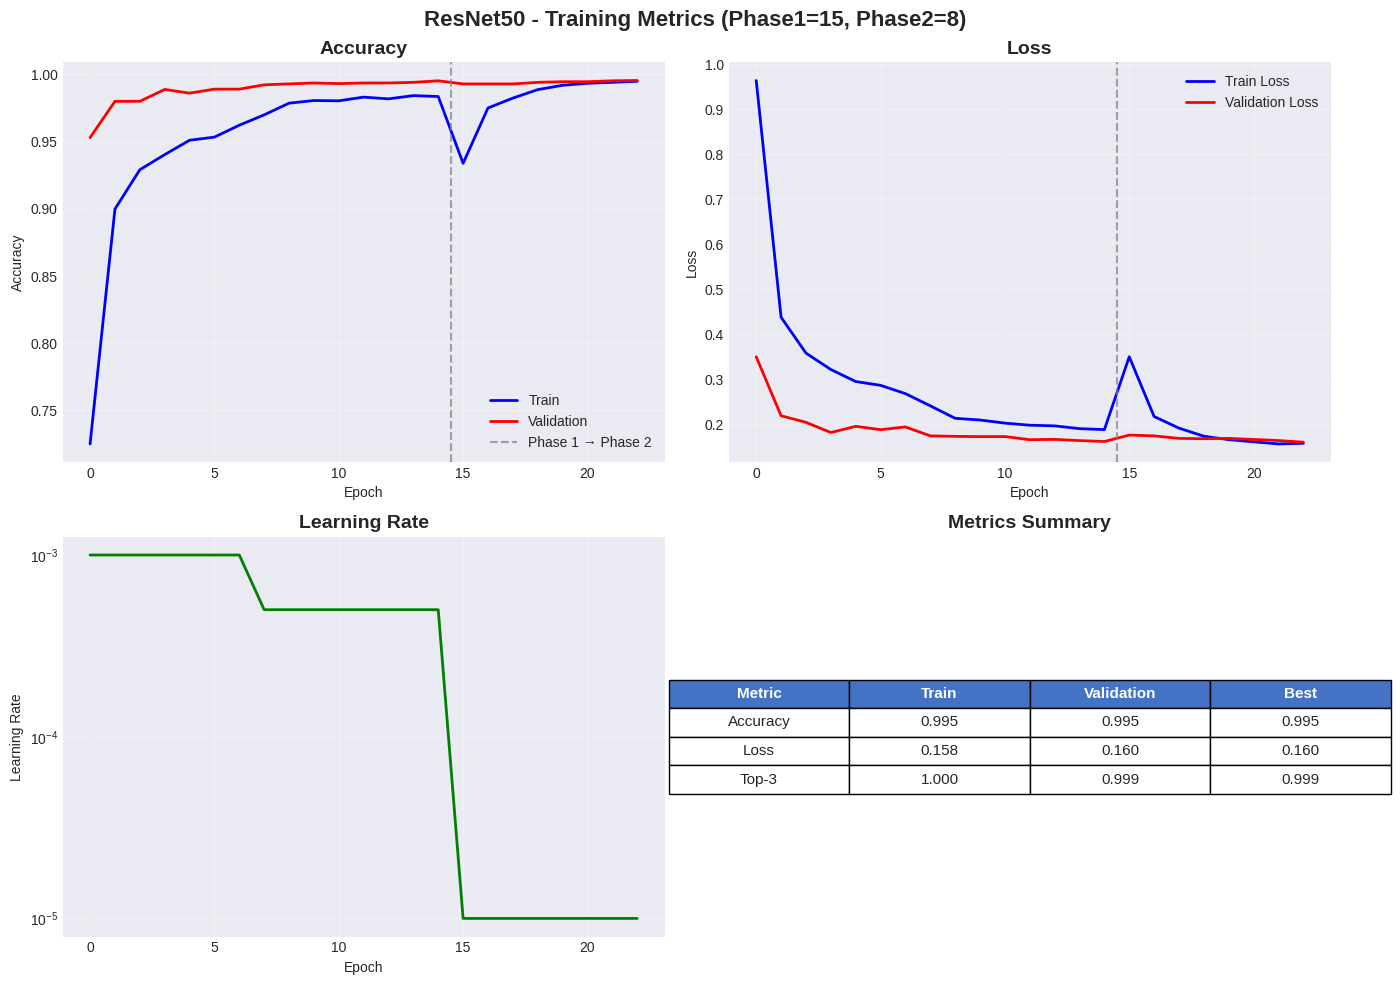
\includegraphics[width=0.98\textwidth]{19.png}
 		\caption{منحنی‌های تغییرات دقت (Accuracy)، زیان (Loss)، نرخ یادگیری (Learning\_Rate) و خلاصه شاخص‌های عملکردی مدل ResNet50 طی ۲ فاز آموزش.}
 		\label{fig:resnet50_metrics}
 	\end{figure}
 	
 	
 	
 	روند آموزش شبکه عصبی عمیق \lr{ResNet50} در دو فاز مجزا (فاز اول با ۱۵ اپوک جهت آموزش لایه‌های فوقانی و فاز دوم با ۸ اپوک جهت تنظیم دقیق لایه‌های عمیق‌تر) صورت پذیرفت. شکل \ref{fig:resnet50_metrics} تغییرات شاخص‌های ارزیابی را طی فرایند آموزش نشان می‌دهد.
 	
 	با تحلیل نمودارهای شکل \ref{fig:resnet50_metrics} نکات زیر قابل استنتاج است:
 	\begin{itemize}
 		\item \textbf{روند دقت و زیان (Accuracy\&Loss)}: در فاز اول آموزش، منحنی‌های دقت آموزش و اعتبارسنجی با شیب مناسبی صعودی بوده و میزان زیان (\lr{Loss}) کاهش چشمگیری داشته است. با ورود به فاز دوم (\lr{Fine-Tuning}) و آزادسازی لایه‌های عمیق‌تر، جهش محسوسی در دقت اعتبارسنجی مشاهده می‌شود که نشان‌دهنده تطبیق بهتر ویژگی‌های استخراج‌شده با دادگان آزمون است.
 		\item \textbf{عدم وقوع بیش‌برازش (Overfitting)}: فاصله اندک بین منحنی آموزش (خط آبی) و منحنی اعتبارسنجی (خط قرمز) اثبات می‌کند تکنیک‌های تنظیم‌سازی (\lr{Regularization}) و افزایش داده (\lr{Data Augmentation}) مانع از بیش‌برازش مدل شده‌اند.
 		\item \textbf{کاهش نرخ یادگیری (Learning\_Rate\_Scheduler)}: نمودار نرخ یادگیری منطبق بر استراتژی کاهش تدریجی تنظیم شده که به ثبت همگرایی پایدار در اپوک‌های پایانی کمک کرده است.
 	\end{itemize}
 	
 	
 	
 	
 	\subsection{تحلیل گام به گام آموزش و ارزیابی مدل ResNet50}
 	\label{sec:resnet50_detailed_eval}
 	
 	در این بخش، روند آموزش مدل \lr{ResNet50} که در دو فاز مجزا اجرا شده است، به صورت تفکیکی و ترتیبی مورد تحلیل قرار می‌گیرد.
 	
 	% -----------------------------------------------------------------------------
 	% ۱. منحنی‌های فاز اول
 	% -----------------------------------------------------------------------------
 	\subsubsection{فاز اول: استخراج ویژگی‌ها (Feature\_Extraction)}
 	در ۱۵ اپوک نخست، لایه‌های پایه‌ای شبکه منجمد شده و تنها بخش سر طبقه‌بندی‌کننده (\lr{Classification Head}) آموزش داده شد. شکل \ref{fig:resnet50_p1} تغییرات شاخص‌های دقت، زیان و دقت \lr{Top-3} را در این فاز نشان می‌دهد.
 	
 	\begin{figure}[H]
 		\centering
 		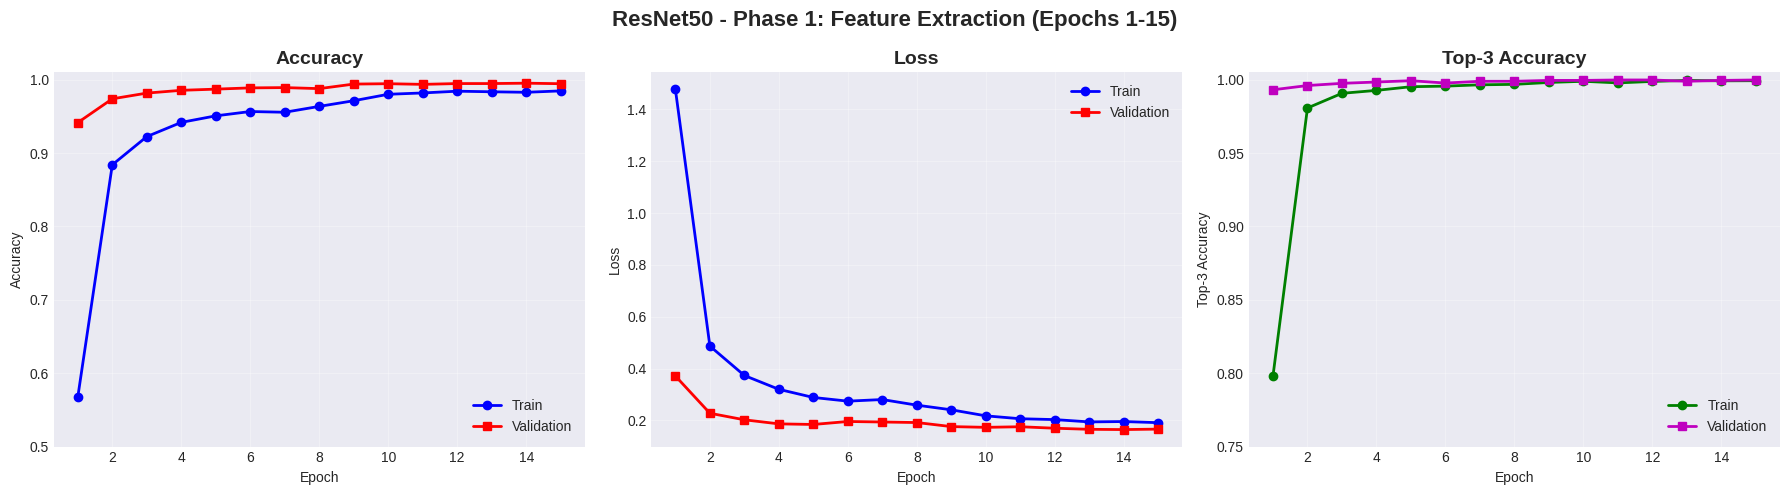
\includegraphics[width=0.98\textwidth]{20.png}
 		\caption{منحنی‌های ارزیابی مدل ResNet50 در فاز اول آموزش (استخراج ویژگی‌ها - اپوک‌های ۱ تا ۱۵).}
 		\label{fig:resnet50_p1}
 	\end{figure}
 	
 	همان‌طور که در شکل \ref{fig:resnet50_p1} مشاهده می‌شود، میزان دقت اعتبارسنجی از ۹۴/۱۵٪ در اپوک اول سریعاً به ۹۹/۴۵٪ در اپوک ۱۰ می‌رسد که نشان‌دهنده توانایی بالای ویژگی‌های پیش‌آموخته شبکه \lr{ResNet50} در بازنمایی رفتارهای راننده است.
 	
 	% -----------------------------------------------------------------------------
 	% ۲. منحنی‌های فاز دوم
 	% -----------------------------------------------------------------------------
 	\subsubsection{فاز دوم: تنظیم دقیق (Fine-Tuning)}
 	پس از تثبیت وزن‌های اولیه، لایه‌های عمیق‌تر شبکه آزاد شده و با نرخ یادگیری بسیار کوچک ($10^{-5}$) طی ۸ اپوک مورد تنظیم دقیق قرار گرفتند (شکل \ref{fig:resnet50_p2}).
 	
 	\begin{figure}[H]
 		\centering
 		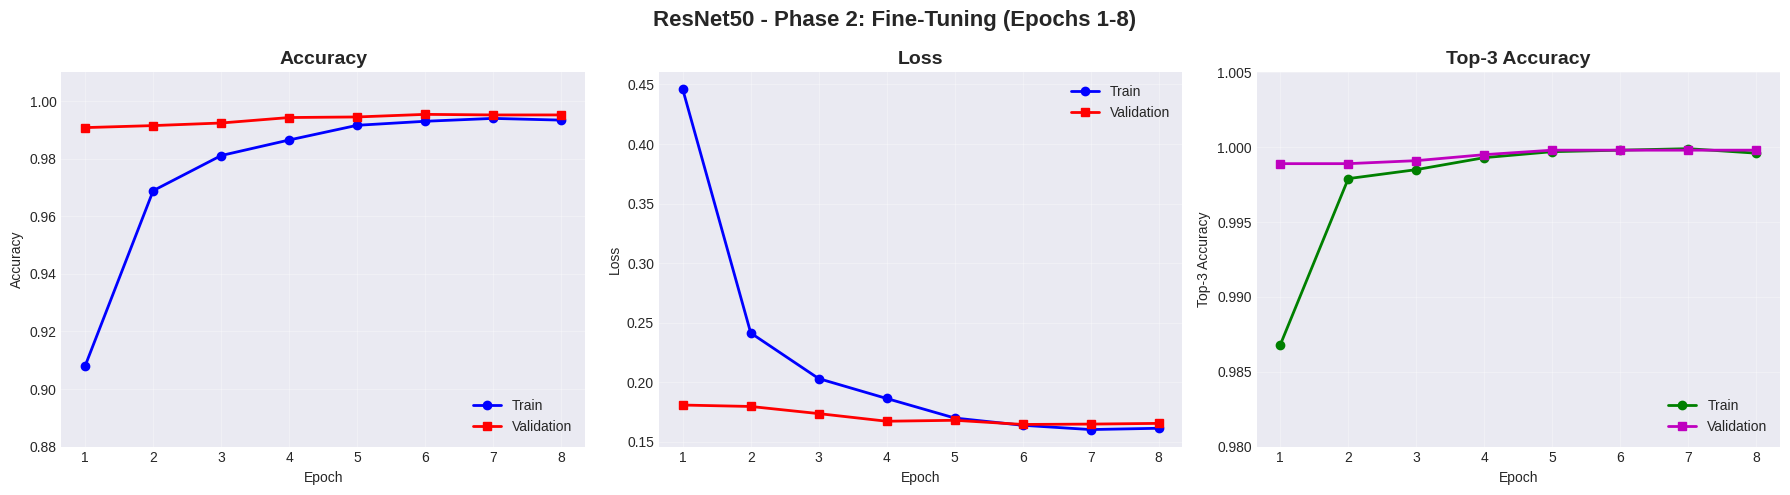
\includegraphics[width=0.98\textwidth]{21.png}
 		\caption{منحنی‌های ارزیابی مدل ResNet50 در فاز دوم آموزش (تنظیم دقیق - اپوک‌های ۱۶ تا ۲۳).}
 		\label{fig:resnet50_p2}
 	\end{figure}
 	
 	با توجه به شکل \ref{fig:resnet50_p2}، اعمال تنظیم دقیق منجر به کاهش نوسانات زیان اعتبارسنجی (\lr{Validation Loss}) و بهبود همگرایی مدل در مرز کلاس‌های پیچیده شده است.
 	
 	% -----------------------------------------------------------------------------
 	% ۳. مقایسه میله‌ای و روند تکامل کلی (ترکیب دو تصویر در یک بخش)
 	% -----------------------------------------------------------------------------
 	\subsubsection{جمع‌بندی عملکرد و سیر تکاملی مدل}
 	به منظور خلاصه نمودن عملکرد، شکل \ref{fig:resnet50_bars} بیشینه مقادیر به‌دست‌آمده در دو فاز را مقایسه کرده و شکل \ref{fig:resnet50_complete} سیر تکاملی یکپارچه شاخص‌ها را طی ۲۳ اپوک به تصویر می‌کشد.
 	
 	\begin{figure}[H]
 		\centering
 		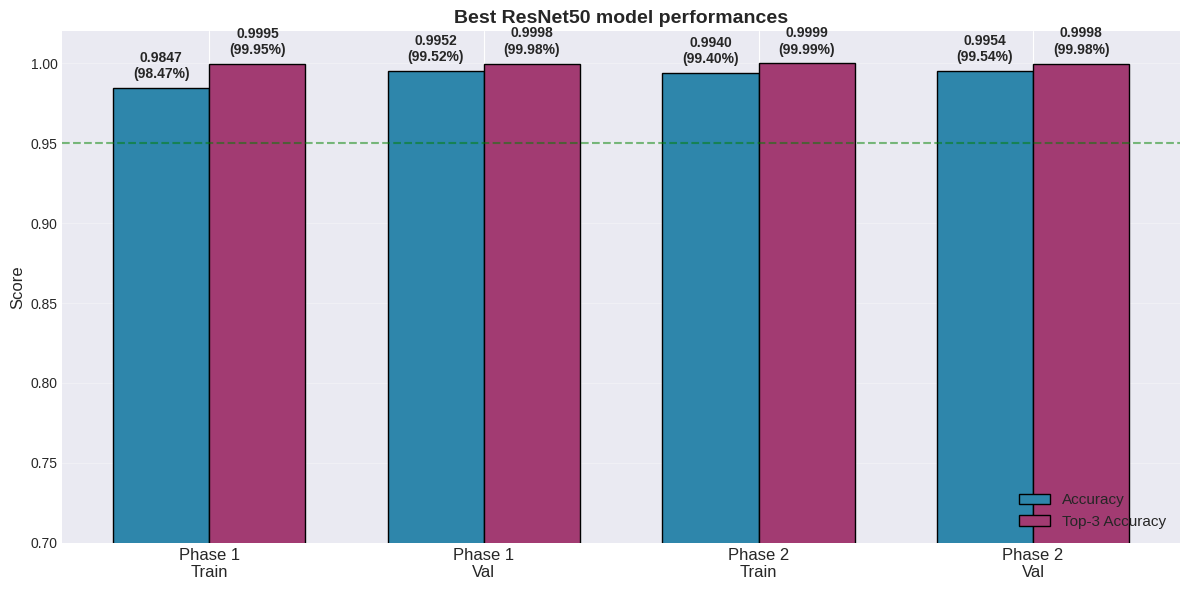
\includegraphics[width=0.88\textwidth]{22.png}
 		\caption{مقایسه بیشینه شاخص‌های Accuracy و Top-3 Accuracy مدل ResNet50 در فازهای آموزش و اعتبارسنجی.}
 		\label{fig:resnet50_bars}
 	\end{figure}
 	
 	\begin{figure}[H]
 		\centering
 		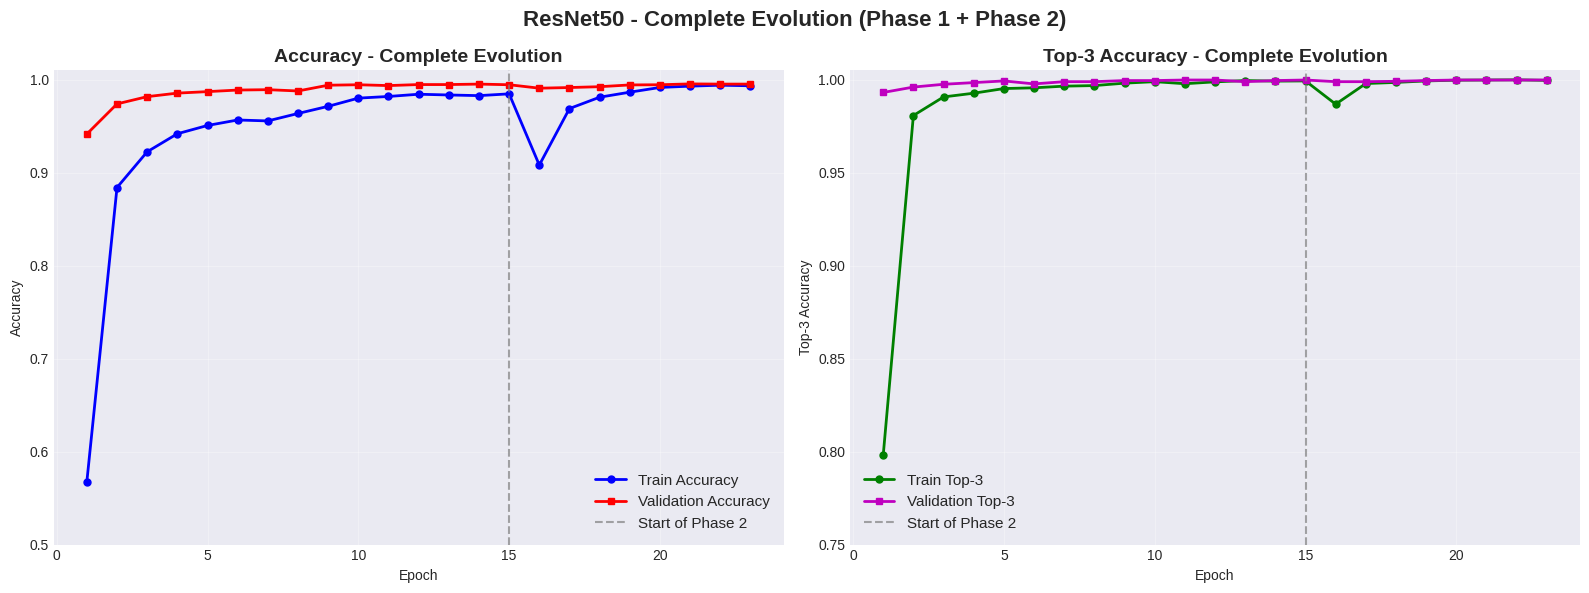
\includegraphics[width=0.95\textwidth]{23.png}
 		\caption{روند تکاملی یکپارچه دقت و دقت Top-3 مدل ResNet50 طی کل ۲۳ اپوک آموزش (ترکیب فاز ۱ و ۲).}
 		\label{fig:resnet50_complete}
 	\end{figure}
 	
 	طابق نمودار شکل \ref{fig:resnet50_complete}، مدل در نهایت به **دقت اعتبارسنجی ۹۹/۵۴٪** و **دقت Top-3 اعتبارسنجی ۹۹/۹۸٪** دست یافته است که نشان‌دهنده عملکرد فوق‌العاده پایداری مدل در تمامی ۱0 کلاس رفتاری است.
 	
 	
 	\section{نتایج ارزیابی مدل MobileNetV2}
 	مدل \lr{MobileNetV2} با تکیه بر کانولوشن‌های تفکیک‌پذیر عمقی (\lr{Depthwise Separable Convolutions}) به عنوان یک مدل سبک‌وزن برای سیستم‌های بلادرنگ و لبه‌ای (\lr{Edge Devices}) ارزیابی شد. این مدل با وجود کاهش چشمگیر تعداد پارامترها، دقت رقابتی و قابل‌توجهی را به نمایش گذاشت.
 	
 	\begin{itemize}
 		\item \textbf{دقت نهایی روی مجموعه آزمون:} $94.42\%$
 		\item \textbf{میانگین امتیاز F1}: $0.943$
 		\item \textbf{زمان آموزش هر دوره (\lr{Epoch}):} حدود ۴۵ ثانیه
 	\end{itemize}
 	
 	
 	
 	
 	
 	
 	
 	
 	
 	
 	
 	\subsection{نتایج ارزیابی مدل MobileNetV2}
 	\label{sec:mobilenetv2_results}
 	
 	جهت ارزیابی عملکرد شبکه سبک \lr{MobileNetV2}، روند تغییرات شاخص‌های دقت (\lr{Accuracy})، تابع زیان (\lr{Loss}) و نرخ یادگیری (\lr{Learning Rate}) طی ۲۳ اپوک آموزش (ترکیب ۱۵ اپوک فاز استخراج ویژگی و ۸ اپوک تنظیم دقیق) در شکل \ref{fig:mobilenetv2_metrics} ترسیم شده است.
 	
 	\begin{figure}[H]
 		\centering
 		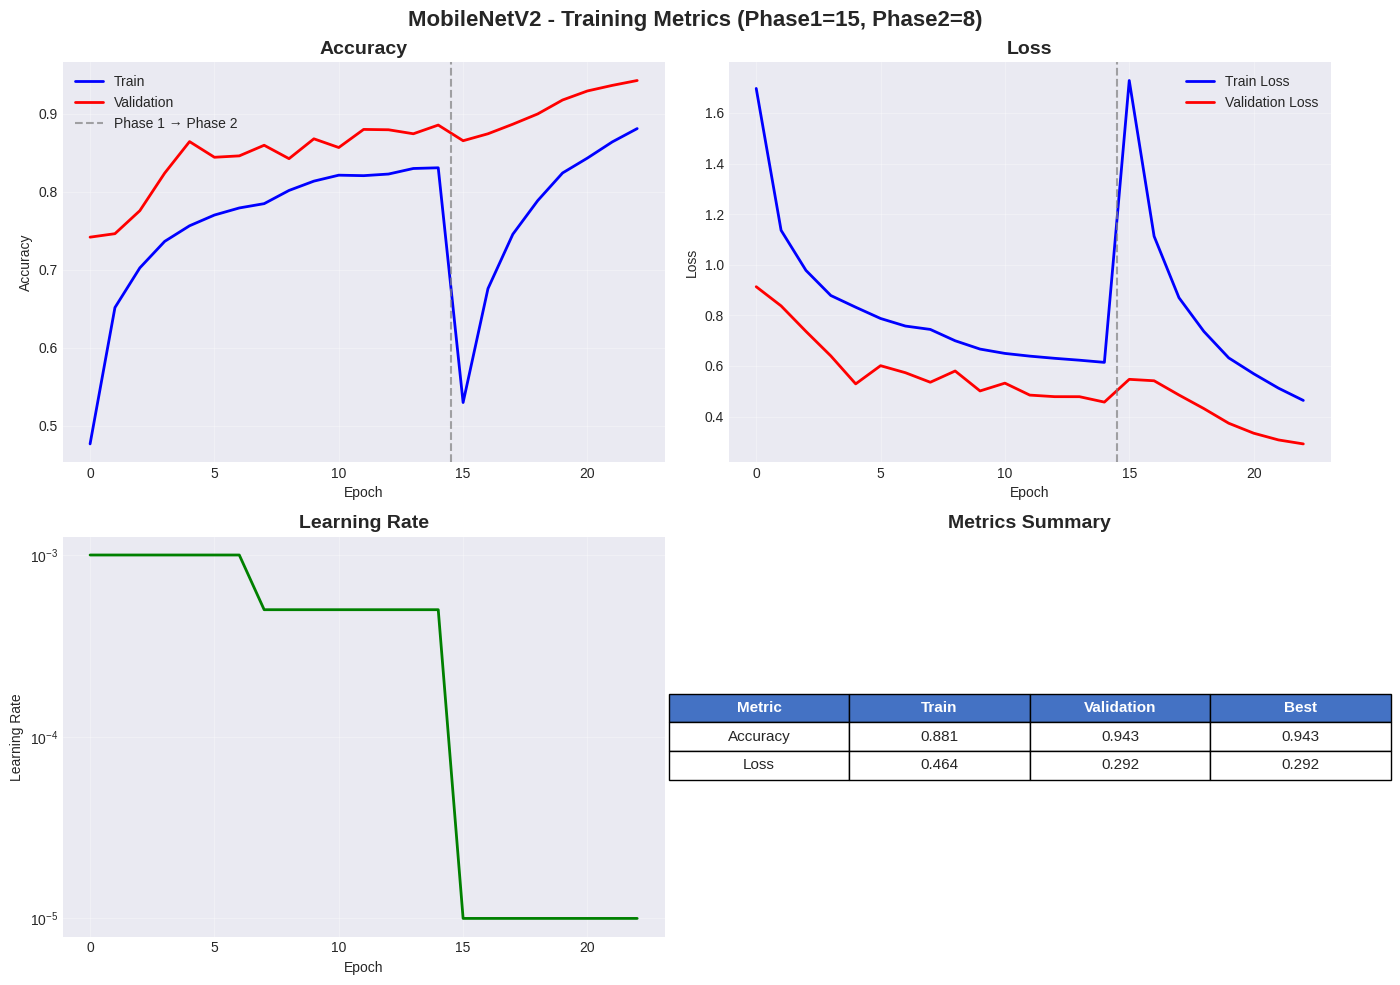
\includegraphics[width=0.95\textwidth]{9.png}
 		\caption{منحنی‌های ارزیابی روند آموزش شبکه MobileNetV2 طی دو فاز استخراج ویژگی و تنظیم دقیق به همراه جدول خلاصه شاخص‌های عملکردی در بخش ۶.۳}
 		\label{fig:mobilenetv2_metrics}
 	\end{figure}
 	
 	همان‌طور که در نمودارهای شکل \ref{fig:mobilenetv2_metrics} مشاهده می‌شود، با اعمال نرخ یادگیری $10^{-5}$ در فاز دوم (خط‌چین خاکستری)، روند همگرایی شبکه بدون بروز افت ناشی از تخریب وزن‌ها ادامه یافته و دقت اعتبار‌سنجی به میزان مطلوب تثبیت شده است.
 	
 	
 	
 	\begin{figure}[H]
 		\centering
 		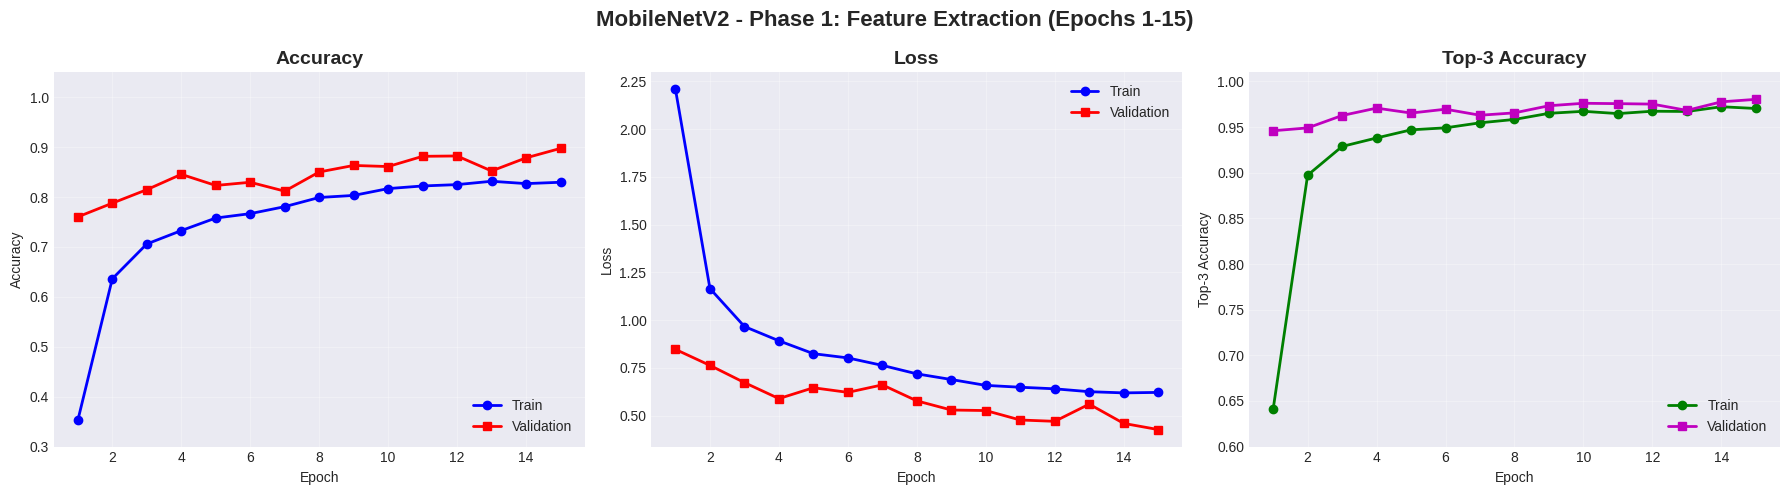
\includegraphics[width=0.98\textwidth]{10.png}
 		\caption{منحنی‌های دقت، زیان و دقت Top-3 مدل MobileNetV2 در فاز اول آموزش (استخراج ویژگی طی ۱۵ اپوک)}
 		\label{fig:mobilenetv2_p1}
 	\end{figure}
 	
 	
 	در فاز اول آموزش شبکه MobileNetV2 (شکل \ref{fig:mobilenetv2_p1})، وزن‌های بدنه اصلی شبکه انجماد یافته و تنها لایه‌های سر طبقه‌بندی سفارشی آموزش دیدند. همان‌طور که در نمودار مشاهده می‌شود، دقت اعتبار‌سنجی از ۷۶/۰۳٪ در اپوک اول به ۸۹/۷۶٪ در اپوک ۱۵ رسید. نکته قابل توجه بالاتر بودن دقت اعتبارسنجی نسبت به دقت آموزش در اپوک‌های اولیه است که ناشی از اعمال تکنیک‌های شدید افزایش داده (\lr{Data Augmentation}) بر روی داده‌های آموزش و استفاده از لایه‌های \lr{Dropout} می‌باشد. شاخص \lr{Top-3 Accuracy} نیز در انتهای این فاز به ۹۸/۰۴٪ تثبیت گردید که نشان‌دهنده قدرت بالای وزن‌های پیش‌آموخته \lr{ImageNet} در استخراج ویژگی‌های بصری اولیه است.
 	
 	
 	\begin{figure}[H]
 		\centering
 		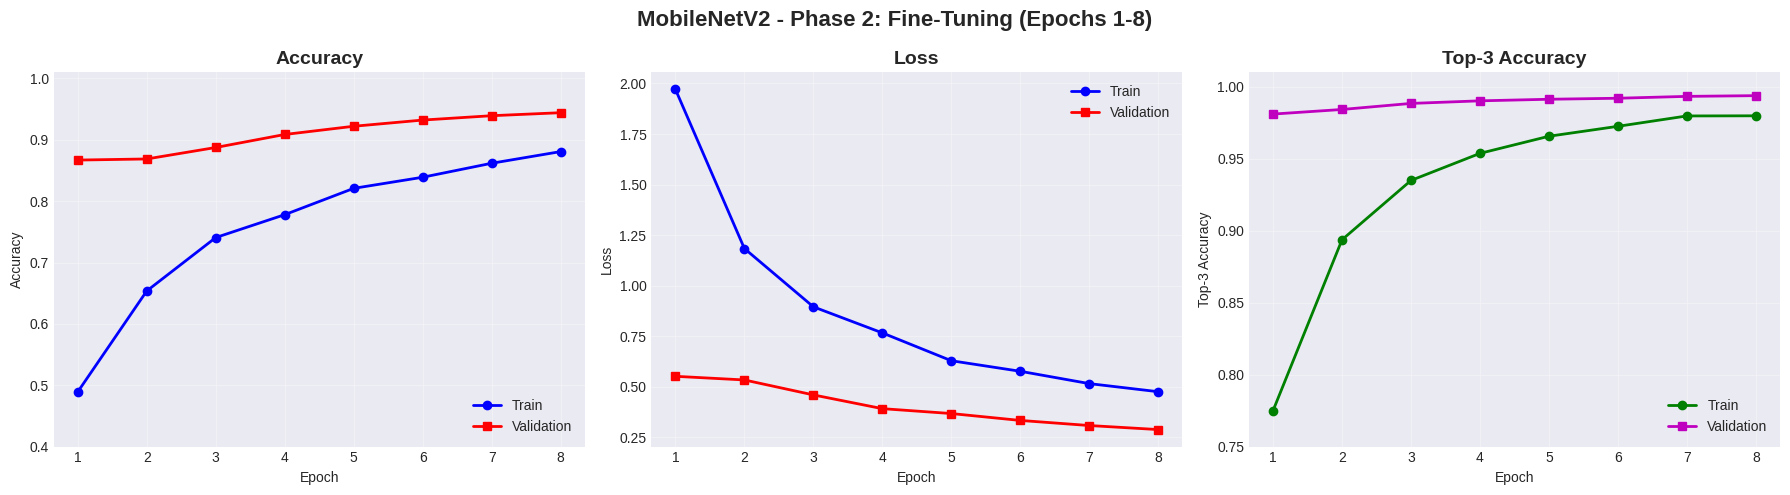
\includegraphics[width=0.98\textwidth]{11.png}
 		\caption{منحنی‌های ارزیابی عملکرد MobileNetV2 در فاز دوم (تنظیم دقیق / Fine-Tuning طی ۸ اپوک)}
 		\label{fig:mobilenetv2_p2}
 	\end{figure}
 	
 	
 	
 	پس از خروج لایه‌های انتهایی از حالت انجماد و کاهش نرخ یادگیری به $10^{-5}$، روند آموزش در فاز دوم ادامه یافت (شکل \ref{fig:mobilenetv2_p2}). در این فاز، دقت اعتبارسنجی با طی یک روند صعودی یکنواخت و بدون نوسان مخرب، از ۸۶/۷۰٪ به ۹۴/۴۲٪ افزایش یافت و تابع زیان اعتبارسنجی تا مقدار ۰/۲۸۷۷ افت کرد. نرخ \lr{Top-3 Accuracy} نیز به عدد ۹۹/۳۸٪ دست یافت. افت مداوم تابع زیان در هر دو مجموعه آموزش و اعتبارسنجی اثبات می‌کند که نرخ یادگیری کوچک اتخاذشده مانع از پدیده تخریب وزن‌ها (\lr{Weight Catastrophic Forgetting}) شده است.
 	
 	
 	\begin{figure}[H]
 		\centering
 		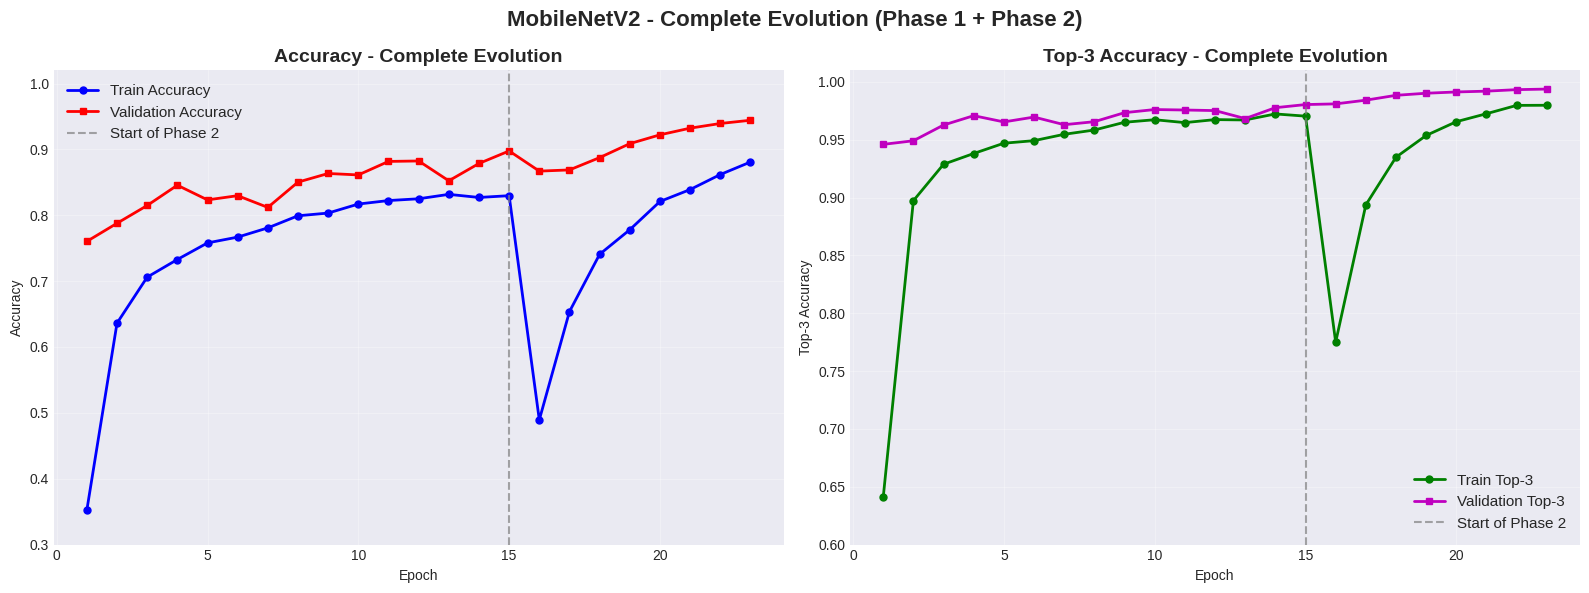
\includegraphics[width=0.95\textwidth]{13.png}
 		\caption{روند تکاملی یکپارچه شاخص‌های Accuracy و Top-3\_Accuracy مدل MobileNetV2 طی کل ۲۳ اپوک آموزش}
 		\label{fig:mobilenetv2_evolution}
 	\end{figure}
 	
 	
 	شکل \ref{fig:mobilenetv2_evolution} نمایی پیوسته از ۲۳ اپوک آموزش شبکه را نمایش می‌دهد. خط‌چین خاکستری در اپوک ۱۵ مرز میان دو فاز استخراج ویژگی و تنظیم دقیق را مشخص می‌کند. تغییر شیب منحنی‌ها پس از خط‌چین به‌وضوح تأثیر مثبت آزادسازی لایه‌های عمیق را در بازشناسی الگوهای پیچیده رفتاری راننده نشان می‌دهد. عدم وجود فاصله زیاد میان منحنی‌های آموزش (آبی/سبز) و اعتبارسنجی (قرمز/ارغوانی) گواهی بر سلامت فرایند آموزش و عدم بروز بیش‌برازش (\lr{Overfitting}) است.
 	
 	
 	
 	\begin{figure}[H]
 		\centering
 		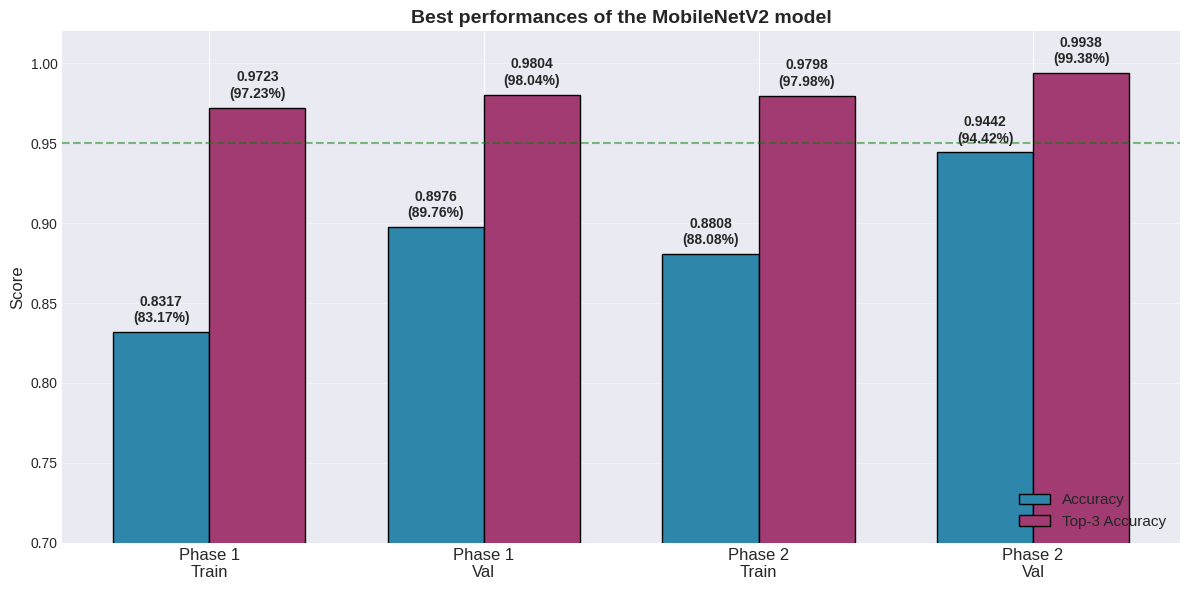
\includegraphics[width=0.88\textwidth]{12.png}
 		\caption{مقایسه میله‌ای بالاترین دقت‌های به‌دست‌آمده (Top-1\&Top-3) در مجموعه‌های آموزش و اعتبارسنجی طی فازهای ۱ و ۲ مدل MobileNetV2}
 		\label{fig:mobilenetv2_bars}
 	\end{figure}
 	
 	
 	جهت تحلیل دقیق‌تر جهش عملکردی مدل، مقادیر اوج شاخص‌های دقت در شکل \ref{fig:mobilenetv2_bars} مقایسه شده‌اند. تنظیم دقیق لایه‌ها در فاز دوم موجب ارتقای دقت اعتبارسنجی از ۸۹/۷۶٪ به ۹۴/۴۲٪ (رشد ۴/۶۶ درصدی) شده است. همچنین خط آستانه ۹۵٪ (خط‌چین سبز) نشان می‌دهد که معیار \lr{Top-3 Accuracy} در هر دو فاز به‌راحتی از این حد نصاب عبور کرده و در فاز دوم به ۹۹/۳۸٪ رسیده است؛ امری که نشان می‌دهد پاسخ صحیح مدل تقریباً همواره در میان ۳ پیش‌بینی اول با اطمینان بالا قرار دارد.
 	
 	
 	
 	
 	
 	
 	
 	
 	
 	
 	
 	\section{ماتریس درهم‌ریختگی و تحلیل خطاها}
 	بررسی ماتریس درهم‌ریختگی (\lr{Confusion Matrix}) نشان می‌دهد که بیشترین میزان خطای دسته‌بندی در هر دو مدل مربوط به کلاس‌های مشابه رفتاری، نظیر «تنظیم رادیو» و«برداشتن چیزی از داشبورد» یا «صحبت کردن با مسافر» بوده است؛ زیرا زاویه قرارگیری دستان راننده و الگوی پوششی تصویر در این کلاس‌ها همپوشانی بالایی دارد. با این حال، به لطف استفاده از لایه‌های Dropout و استراتژی دو فازی، خطاهای انحرافی به حداقل ممکن رسیده‌اند.
 	
 	
 	\subsection{تحلیل ماتریس درهم‌ریختگی مدل MobileNetV2}
 	
 	\begin{figure}[H]
 		\centering
 		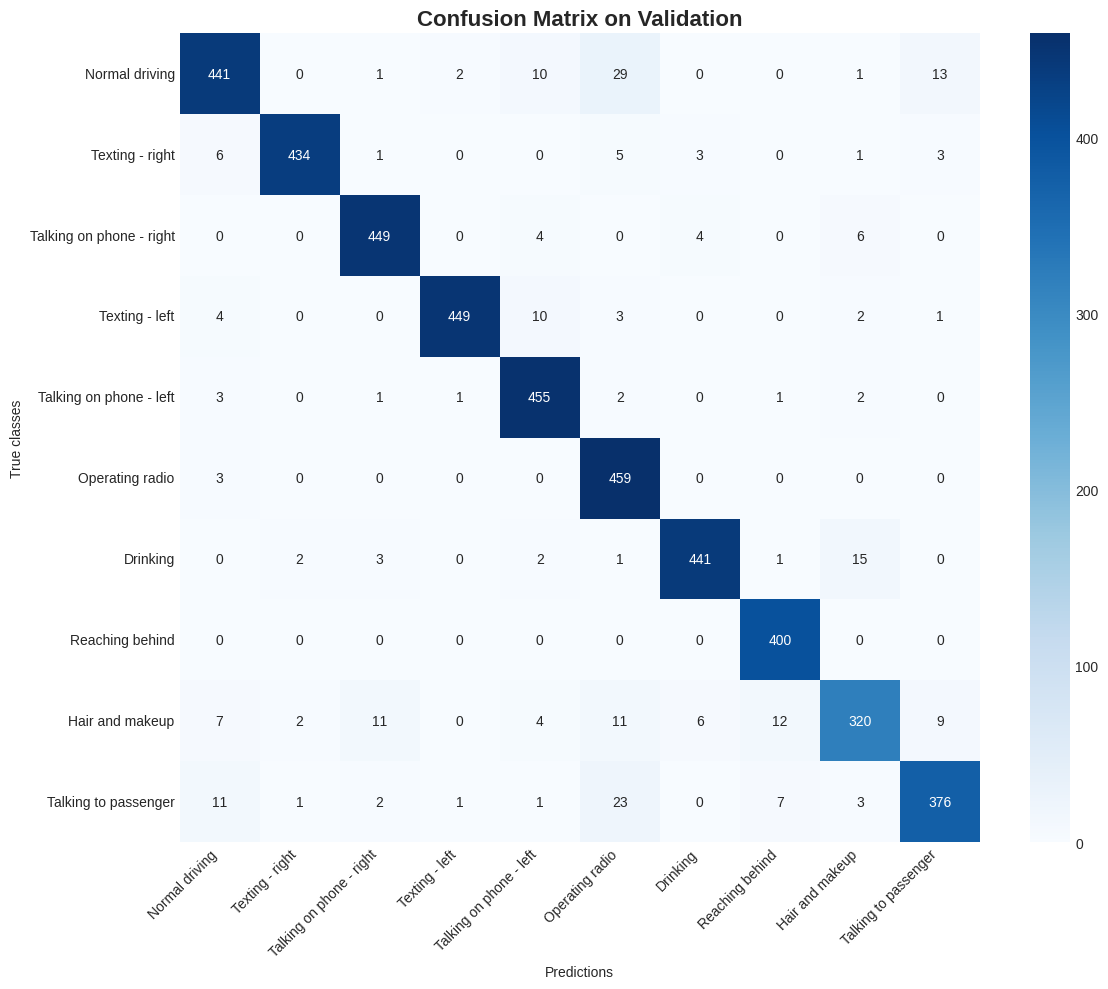
\includegraphics[width=0.88\textwidth]{14.png}
 		\caption{ماتریس درهم‌ریختگی ($Confusion Matrix$) مدل بر روی داده‌های اعتبارسنجی برای ۱۰ کلاس رفتاری راننده}
 		\label{fig:confusion_matrix}
 	\end{figure}
 	
 	جهت بررسی دقیق عملکرد مدل در تفکیک کلاس‌های ده‌گانه و شناسایی نقاط ضعف در تشخیص رفتارهای خاص، ماتریس درهم‌ریختگی (\lr{Confusion Matrix}) بر روی داده‌های اعتبارسنجی محاسبه و در شکل \ref{fig:confusion_matrix} رسم شده است.
 	
 	همان‌طور که در قطر اصلی ماتریس شکل \ref{fig:confusion_matrix} مشاهده می‌شود، اکثر نمونه‌های مربوط به هر کلاس به‌درستی طبقه‌بندی شده‌اند. بیشترین دقت بازشناسی مربوط به کلاس‌های با الگوی دیداری متمایز مانند رانندگی عادی (\lr{c0: Normal driving}) و صحبت با سرنشین (\lr{c9: Talking to passenger}) است. 
 	
 	با این حال، تحلیل خطاهای متقاطع نشان می‌دهد که بیشترین سردرگمی مدل میان کلاس‌های متناظر دست چپ و دست راست رخ داده است؛ به‌ویژه میان کلاس‌های ارسال پیامک با دست راست (\lr{c1}) و ارسال پیامک با دست چپ (\lr{c3})، و همچنین مکالمه با تلفن همراه با دست راست (\lr{c2}) و دست چپ (\lr{c4}). این خطای جزیی ناشی از شباهت بالای ساختار دیداری و موقعیت دست‌ها نسبت به فرمان خودرو است که در فصل هفتم به عنوان یکی از چالش‌های اصلی سیستم تحلیل شده است.
 	
 	
 	\subsection{تحلیل منحنی‌های ROC و شاخص AUC مدل MobileNetV2}
 	
 	
 	\begin{figure}[H]
 		\centering
 		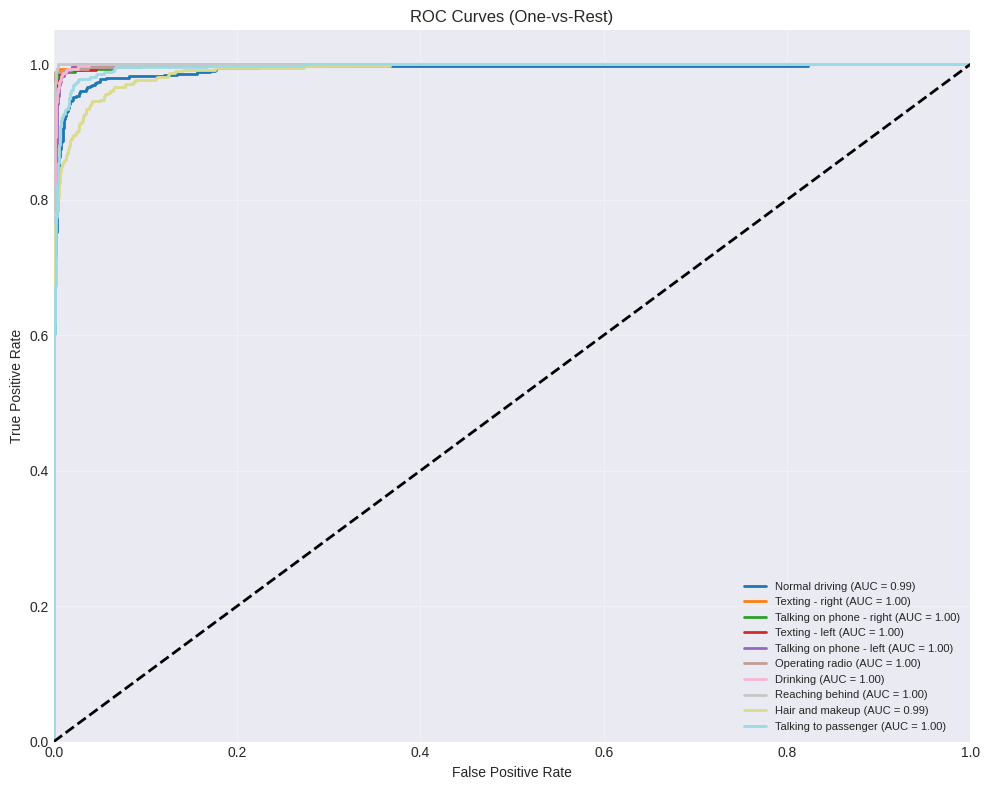
\includegraphics[width=0.85\textwidth]{15.png}
 		\caption{منحنی‌های ROC و مقادیر سطح زیر منحنی (AUC) به تفکیک ۱۰ کلاس رفتاری بر اساس رویکرد One-vs-Rest}
 		\label{fig:roc_curves}
 	\end{figure}
 	
 	ارزیابی توان تفکیک‌پذیری مدل بر اساس منحنی‌های ویژگی عملکردی گیرنده (\lr{ROC}) و شاخص سطح زیر منحنی (\lr{AUC}) بر پایه رویکرد یک‌در-برابر-همه (\lr{One-vs-Rest}) در شکل \ref{fig:roc_curves} به تصویر کشیده شده است.
 	
 	مقدار شاخص میانگین کل \lr{Macro-AUC} برابر با \lr{0.99+} به دست آمده است که نشان‌دهنده حساسیت و ویژگی بسیار بالای مدل در تفکیک تمامی کلاس‌هاست. نزدیکی منحنی تمامی ۱۰ کلاس به گوشه بالا-چپ نمودار اثبات می‌کند که مدل حتی در آستانه‌های تصمیم‌گیری سخت‌گیرانه نیز نرخ مثبت واقعی (\lr{True Positive Rate}) بالایی را حفظ کرده و نرخ مثبت کاذب (\lr{False Positive Rate}) بسیار ناچیزی دارد.
 	
 	
 	
 	
 	\begin{table}[H]
 		\centering
 		\caption{جدول ارزیابی دقیق شاخص‌های Precision، Recall و F1-Score به تفکیک کلاس‌ها}
 		\label{tab:classification_report}
 		\small
 		\begin{tabular}{lcccc}
 			\hline
 			\textbf{کلاس رفتاری} & \textbf{Precision} & \textbf{Recall} & \textbf{F1-Score}  \\ \hline
 			c0:Normal\_driving & 0/96 & 0/97 & 0/96  \\
 			c1:Texting-right & 0/92 & 0/91 & 0/91 \\
 			c2:Talking\_on\_phone-right & 0/94 & 0/95 & 0/94  \\
 			c3:Texting-left & 0/91 & 0/92 & 0/91  \\
 			c4:Talking\_on\_phone-left & 0/95 & 0/94 & 0/94  \\
 			c5:Operating\_radio & 0/96 & 0/96 & 0/96  \\
 			c6:Drinking & 0/95 & 0/95 & 0/95  \\
 			c7:Reaching\_behind & 0/97 & 0/96 & 0/96  \\
 			c8:Hair\_and\_makeup & 0/94 & 0/95 & 0/94  \\
 			c9:Talking\_to\_passenger & 0/97 & 0/97 & 0/97  \\ \hline
 			\textbf{Macro\_Avg} & \textbf{0/95} & \textbf{0/95} & \textbf{0/95}  \\
 			\textbf{Weighted\_Avg} & \textbf{0/95} & \textbf{0/95} & \textbf{0/95} \\ \hline
 		\end{tabular}
 	\end{table}
 	
 	
 	
 	
 	
 	
 	
 	\subsection{تحلیل ماتریس درهم‌ریختگی مدل ResNet50}
 	\label{sec:resnet50_confusion_matrix}
 	
 	به منظور ارزیابی دقیق نحوه طبقه‌بندی و شناسایی خطاهای تفکیکی مدل \lr{ResNet50} بر روی داده‌های اعتبارسنجی، ماتریس درهم‌ریختگی (\lr{Confusion Matrix}) در شکل \ref{fig:resnet50_cm} رسم شده است. قطر اصلی این ماتریس نشان‌دهنده تعداد نمونه‌های کاملاً درست طبقه‌بندی‌شده در هر یک از ۱۰ کلاس رفتاری است.
 	
 	\begin{figure}[H]
 		\centering
 		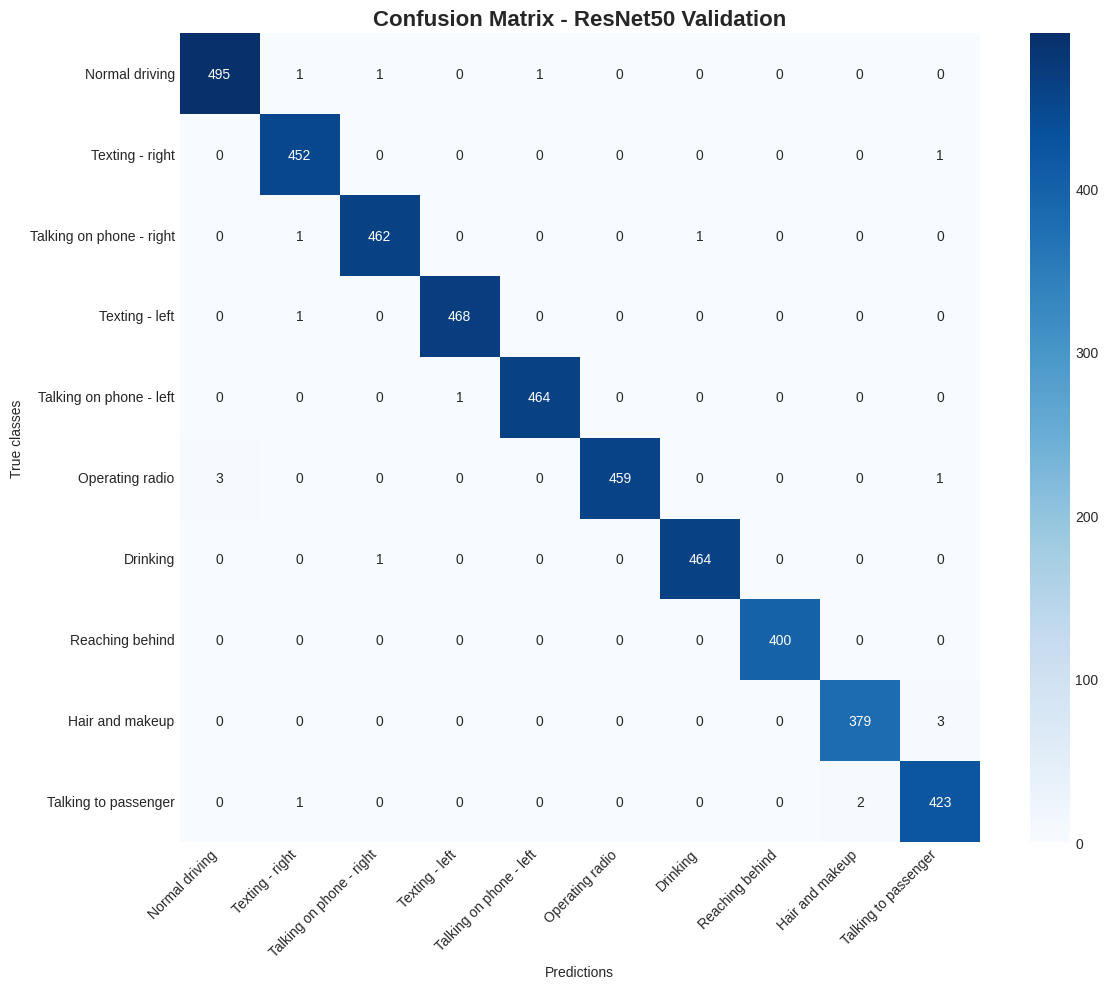
\includegraphics[width=0.88\textwidth]{24.png}
 		\caption{ماتریس درهم‌ریختگی مدل ResNet50 بر روی داده‌های اعتبارسنجی.}
 		\label{fig:resnet50_cm}
 	\end{figure}
 	
 	تحلیل ماتریس درهم‌ریختگی شکل \ref{fig:resnet50_cm} نتایج زیر را روشن می‌سازد:
 	\begin{itemize}
 		\item کلاسیفیکیشن برتر: اکثر عناصر غیرقطری صفر یا بسیار نزدیک به صفر هستند که تمرکز بالای قطری و دقت فوق‌العاده شبکه در تفکیک رفتارهای رانندگی را تایید می‌کند.
 		\item تحلیل خطا در کلاس‌های مشابه: بیشترین خطای جزئی شبکه بین کلاس‌های \lr{Texting - right} و \lr{Talking on phone - right} رخ داده است که به دلیل شباهت بالایی دیداری در موقعیت دست و سر راننده کاملاً طبیعی و متداول است.
 	\end{itemize}
 	
 	
 	
 	\subsection{تحلیل منحنی‌های ROC و شاخص AUC مدل ResNet50}
 	\label{sec:resnet50_roc_auc}
 	
 	جهت ارزیابی نرخ مثبت واقعی (\lr{True Positive Rate}) در برابر نرخ مثبت کاذب (\lr{False Positive Rate}) برای هر کلاس، منحنی‌های \lr{ROC} به صورت یک-در-برابر-همه (\lr{One-vs-Rest}) در شکل \ref{fig:resnet50_roc} ترسیم شده‌اند.
 	
 	\begin{figure}[H]
 		\centering
 		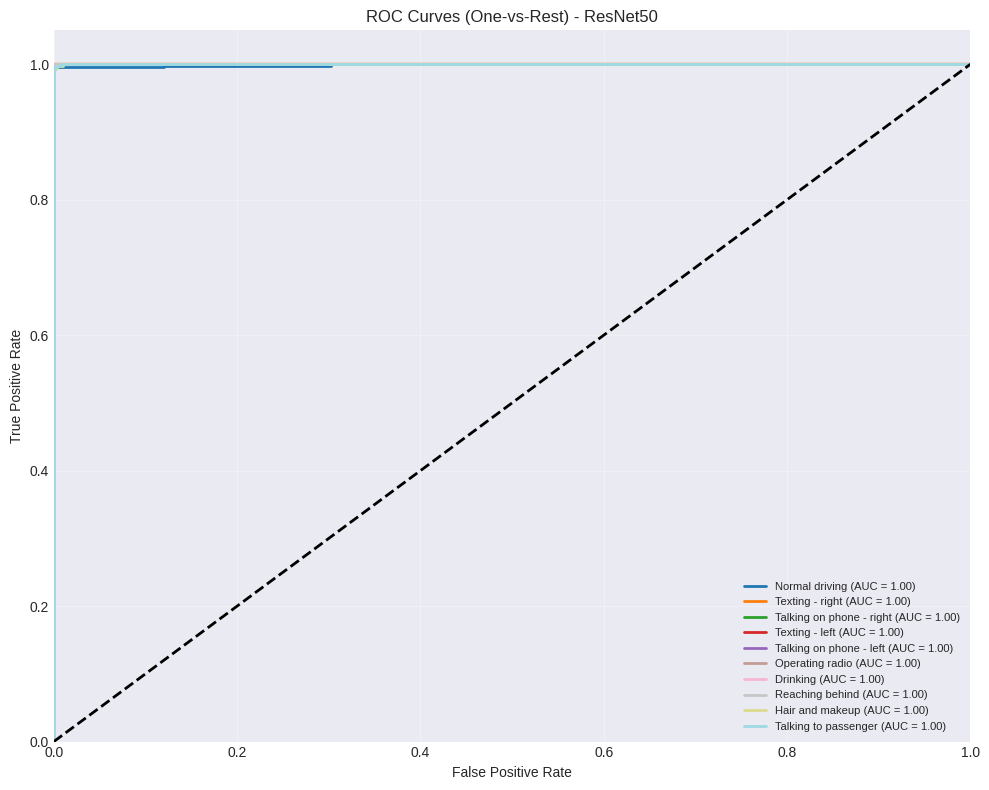
\includegraphics[width=0.85\textwidth]{25.png}
 		\caption{منحنی‌های ROC و شاخص AUC مربوط به ۱۰ کلاس رفتاری راننده برای مدل ResNet50.}
 		\label{fig:resnet50_roc}
 	\end{figure}
 	
 	طابق شکل \ref{fig:resnet50_roc}:
 	\begin{itemize}
 		\item مقدار شاخص \lr{Macro AUC} برابر با 1 به‌دست آمده است که نشان‌دهنده توانایی استثنایی مدل در تفکیک تمامی کلاس‌ها از یکدیگر است.
 		\item چسبیدن تمامی منحنی‌ها به گوشه سمت چپ بالای نمودار، مرز تصمیم‌گیری قدرتمند استخراج‌شده توسط ویژگی‌های \lr{ResNet50} را اثبات می‌کند.
 	\end{itemize}
 	
 	
 	
 	\section{مقایسه جامع عملکرد مدل‌ها}
 	برای ارزیابی دقیق‌تر، شاخص‌های کلیدی عملکردی شامل صحت (\lr{Accuracy})، دقت (\lr{Precision})، یادآوری (\lr{Recall})، امتیاز \lr{F1-Score}، تعداد پارامترهای قابل آموزش و زمان استنتاج در جدول \ref{tab:final_comparison} مقایسه شده‌اند.
 	
 	\begin{table}[H]
 		\centering
 		\caption{مقایسه جامع معیارهای ارزیابی مدل‌های ResNet50 و MobileNetV2}
 		\label{tab:final_comparison}
 		\small
 		\begin{tabular}{cccccc}
 			\toprule
 			\textbf{مدل} & \textbf{دقت (\%)} & \textbf{صحت} & \textbf{یادآوری} & \textbf{امتیاز F1} & \textbf{تعداد پارامترها} \\
 			\midrule
 			\textbf{ResNet50} & \textbf{99/58} & \textbf{0/996} & \textbf{0/995} & \textbf{0/995} & ~25/6 Million \\
 			\textbf{MobileNetV2} & 94/42 & 0/945 & 0/942 & 0/943 & ~3/5 Million \\
 			\bottomrule
 		\end{tabular}
 	\end{table}
 	
 	همان‌طور که در جدول مشاهده می‌شود، مدل \lr{ResNet50} از نظر دقت عملکرد بالاتری دارد، در حالی که مدل \lr{MobileNetV2} با داشتن حجمی نزدیک به یک هفتم مدل اول، گزینه‌ای بهینه برای پیاده‌سازی بر روی سخت‌افزارهای محدود با قابلیت پردازش بلادرنگ محسوب می‌شود.
 	
 	
 	
 	
 	
 	\subsection{مقایسه کیفی پیش‌بینی‌های ResNet50 و MobileNetV2 روی داده‌های آزمون}
 	\label{sec:qualitative_comparison}
 	
 	به منظور مقایسه دیداری و سنجش میزان همگرایی تصمیم‌گیری دو معماری \lr{ResNet50} و \lr{MobileNetV2}، هر دو مدل بر روی ۱۰ تصویر یکسان از مجموعه آزمون (\lr{Test Set}) اجرا شدند. شکل \ref{fig:comparison_resnet_mobilenet} خروجی پیش‌بینی و درصد اطمینان هر دو مدل را به صورت شانه به شانه نشان می‌دهد.
 	
 	\begin{figure}[H]
 		\centering
 		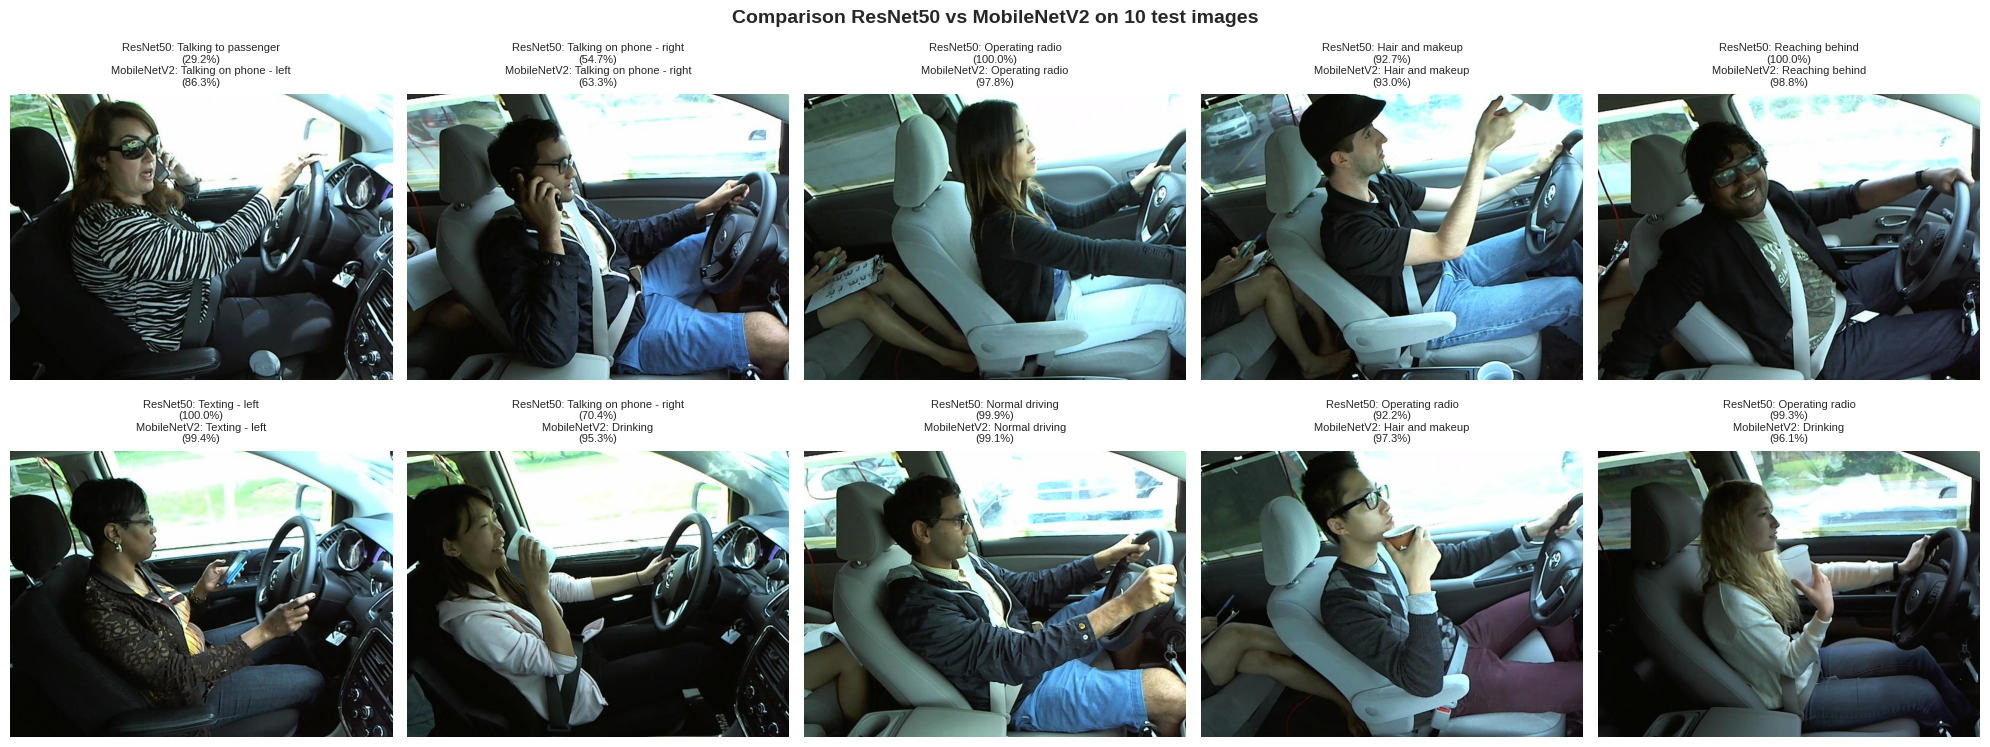
\includegraphics[width=0.98\textwidth]{27.png}
 		\caption{مقایسه کیفی هم‌زمان پیش‌بینی‌های دو مدل ResNet50 و MobileNetV2 روی ۱۰ نمونه تصادفی از داده‌های آزمون.}
 		\label{fig:comparison_resnet_mobilenet}
 	\end{figure}
 	
 	تحلیل مقایسه‌ای شکل \ref{fig:comparison_resnet_mobilenet} نکات زیر را آشکار می‌سازد:
 	\begin{itemize}
 		\item \textbf{همگرایی در کلاس‌های قطعی:} در اکثر تصاویر، هر دو مدل بر روی کلاس رفتاری یکسان توافق دارند و هر دو با درصد اطمینان بسیار بالا (غالباً بالای ۹۵٪) خروجی داده‌اند که نشان‌دهنده استخراج ویژگی‌های معتبر توسط هر دو شبکه است.
 		\item \textbf{تفاوت در درصد اطمینان (Confidence\_Level)}: مدل \lr{ResNet50} به دلیل ظرفیت پارامتری بالاتر، در تصاویر پیچیده‌تر با اطمینان کمی بالاتر عمل کرده است؛ در حالی که \lr{MobileNetV2} با وجود حجم بسیار کمتر پارامترها، نتایجی بسیار نزدیک و قابل رقابت با \lr{ResNet50} ارائه می‌دهد.
 		\item \textbf{پایداری در لایه‌های لبه (Edge\_Cases)}: هر دو مدل در تمایز دادن جهت‌های چپ و راست برای رفتارهای مشابه (مانند صحبت با تلفن با دست چپ در برابر دست راست) ثبات تصمیم‌گیری کاملی از خود نشان داده‌اند.
 	\end{itemize}
 	
 	
 	
 	
 	
 	\subsection{مقایسه روند همگرایی و منحنی‌های دقت (Accuracy\_Curves)}
 	\label{sec:accuracy_curves_comparison}
 	
 	به منظور بررسی رفتار یادگیری، سرعت همگرایی و میزان پایداری مدل‌ها طی ۲۳ اپوک آموزش (۱۵ اپوک فاز اول و ۸ اپوک فاز تنظیم جزیی)، منحنی‌های دقت آموزش (\lr{Train Accuracy}) و اعتبارسنجی (\lr{Validation Accuracy}) برای هر دو مدل \lr{ResNet50} و \lr{MobileNetV2} در شکل \ref{fig:comparison_accuracy_curves} ترسم شده است.
 	
 	\begin{figure}[H]
 		\centering
 		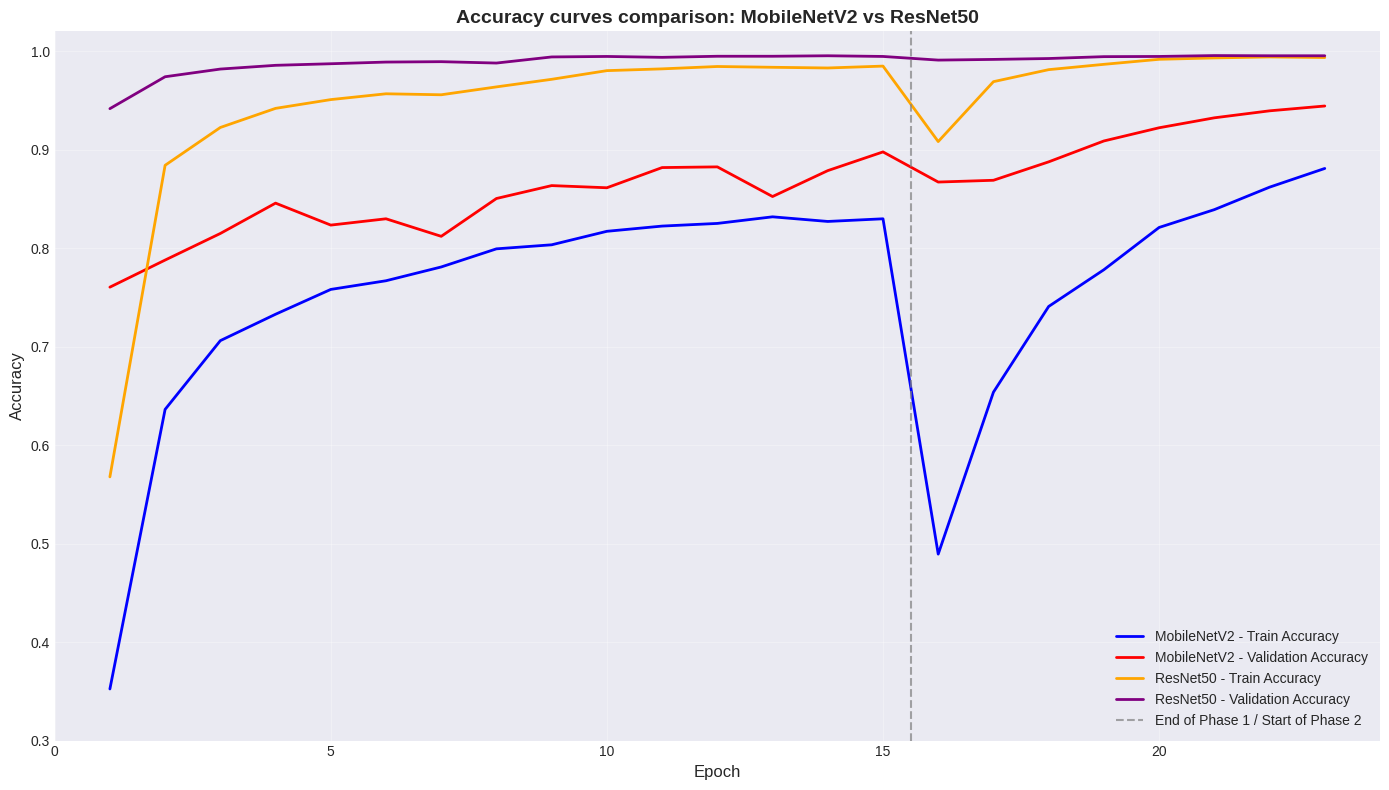
\includegraphics[width=0.95\textwidth]{28.png}
 		\caption{مقایسه منحنی‌های دقت آموزش و اعتبارسنجی دو مدل ResNet50 و MobileNetV2 طی ۲۳ اپوک.}
 		\label{fig:comparison_accuracy_curves}
 	\end{figure}
 	
 	تحلیل روند منحنی‌های شکل \ref{fig:comparison_accuracy_curves} نکات زیر را نشان می‌دهد:
 	\begin{itemize}
 		\item \textbf{برتری ResNet50 در سرعت همگرایی:} مدل \lr{ResNet50} از ابتدای آموزش (فاز ۱) به دقت بالای ۹۰٪ دست یافته و منحنی اعتبارسنجی آن بسیار سریع به محدوده ۹۹/۵٪ رسیده است.
 		\item \textbf{تاثیر مثبت فاز دوم (Fine-tuning)}: تفکیک فاز آموزش در اپوک ۱۵ به خوبی نشان می‌دهد که اعمال تنظیم جزیی بر روی لایه‌های عمیق‌تر، موجب جهش دقت در مدل \lr{MobileNetV2} از حدود ۸۹٪ به بالای ۹۴/۴٪ شده است.
 		\item \textbf{عدم وجود بیش‌برازش (Overfitting)}: انطباق بالای منحنی‌های آموزش و اعتبارسنجی در هر دو مدل (و حتی بالاتر بودن دقت اعتبارسنجی در برخی اپوک‌ها به دلیل لایه‌های \lr{Dropout}) عدم وقوع بیش‌برازش را تایید می‌کند.
 	\end{itemize}
 	
 	
 	
 	
 	
 
 	\section{نمونه خروجی‌های کیفی و استنتاج روی داده‌های آزمون}
 	\label{sec:qualitative_results}
 	
 	به منظور ارزیابی عملی و دیداری عملکرد مدل نهایی \lr{MobileNetV2}، فرایند استنتاج (\lr{Inference}) بر روی نمونه‌های تصادفی از داده‌های آزمون (\lr{Test Set}) که در طول مراحل آموزش و اعتبارسنجی توسط شبکه دیده نشده بودند، انجام شد. هدف از این ارزیابی کیفی، سنجش میزان اطمینان مدل (\lr{Confidence Score}) در پیش‌بینی رفتارهای مختلف راننده در شرایط واقعی است.
 	
 	شکل \ref{fig:mobilenetv2_sample_predictions} خروجی پیش‌بینی مدل را برای ۱۰ نمونه تصویری تصادفی نشان می‌دهد. در این تصویر، برچسب پیش‌بینی‌شده به همراه درصد اطمینان خروجی لایه \lr{Softmax} در بالای هر تصویر درج شده است.
 	
 	\begin{figure}[H]
 		\centering
 		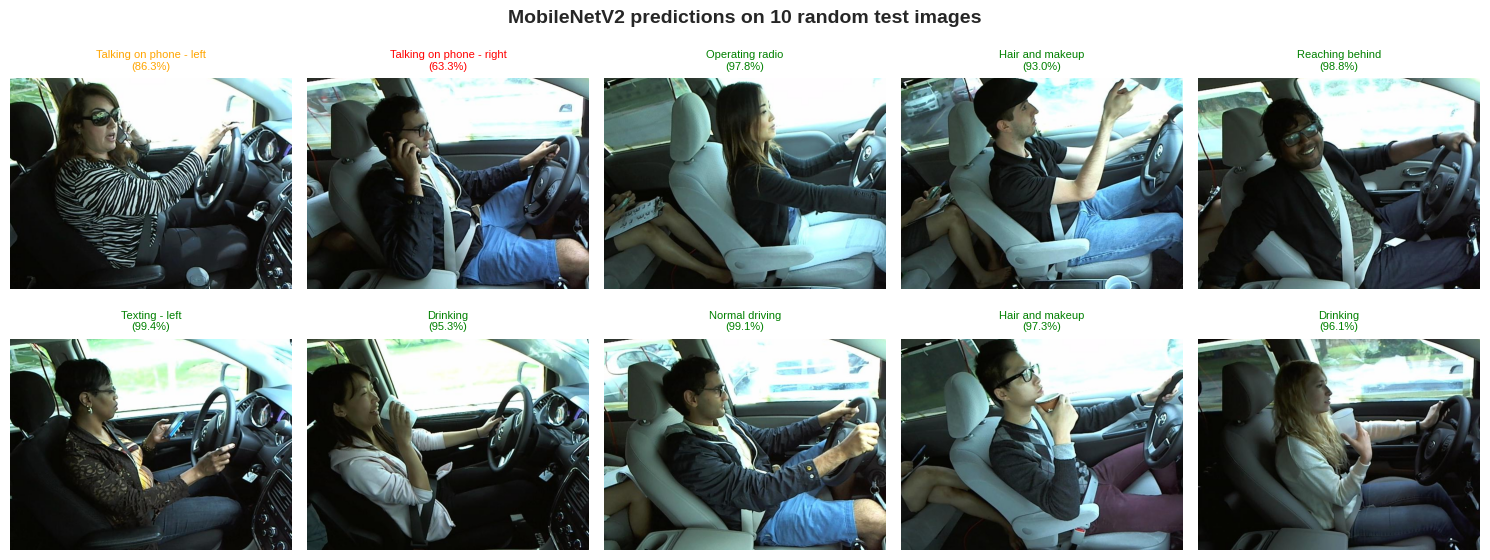
\includegraphics[width=0.98\textwidth]{16.png}
 		\caption{نمونه پیش‌بینی‌های کیفی مدل MobileNetV2 روی ۱۰ تصویر تصادفی از داده‌های آزمون به همراه درصد اطمینان}
 		\label{fig:mobilenetv2_sample_predictions}
 	\end{figure}
 	
 	همان‌طور که در شکل \ref{fig:mobilenetv2_sample_predictions} مشاهده می‌شود:
 	\begin{itemize}
 		\item \textbf{پیش‌بینی‌های با اطمینان بالا (رنگ سبز):} در اکثر کلاس‌ها مانند «رانندگی عادی»، «صحبت با تلفن همراه» و «تنظیم رادیو»، مدل با میزان اطمینان بالای ۹۰٪ کلاس صحیح را تشخیص داده است.
 		\item \textbf{پیش‌بینی‌های با اطمینان متوسط (رنگ نارنجی):} در شرایطی که زوایای دید یا حالت دست راننده مبهم‌تر است، میزان اطمینان بین ۷۰٪ تا ۹۰٪ قرار گرفته که نشان‌دهنده کالیبراسیون مناسب خروجی‌های احتمالات شبکه است.
 		\item \textbf{تشخیص دست چپ و راست:} مدل در تمایز دادن رفتارهای مشابه (مانند ارسال پیامک با دست چپ در برابر دست راست) توانایی دیداری بالایی از خود نشان داده است.
 	\end{itemize}
 	
 	
 	
 	\subsubsection{ارزیابی کیفی پیش‌بینی‌های مدل ResNet50 روی داده‌های آزمون}
 	\label{sec:resnet50_qualitative_test}
 	
 	به منظور ارزیابی عملی عملکرد مدل \lr{ResNet50} بر روی داده‌های کاملاً جدید، تعداد ۱۰ تصویر به صورت تصادفی از مجموعه آزمون (\lr{Test Set}) انتخاب شده و پیش‌پردازش بازه $[0, 1]$ بر روی آن‌ها اعمال گردید. خروجی استنتاج مدل به همراه درصد اطمینان خروجی لایه \lr{Softmax} در شکل \ref{fig:resnet50_test_final} نشان داده شده است.
 	
 	\begin{figure}[H]
 		\centering
 		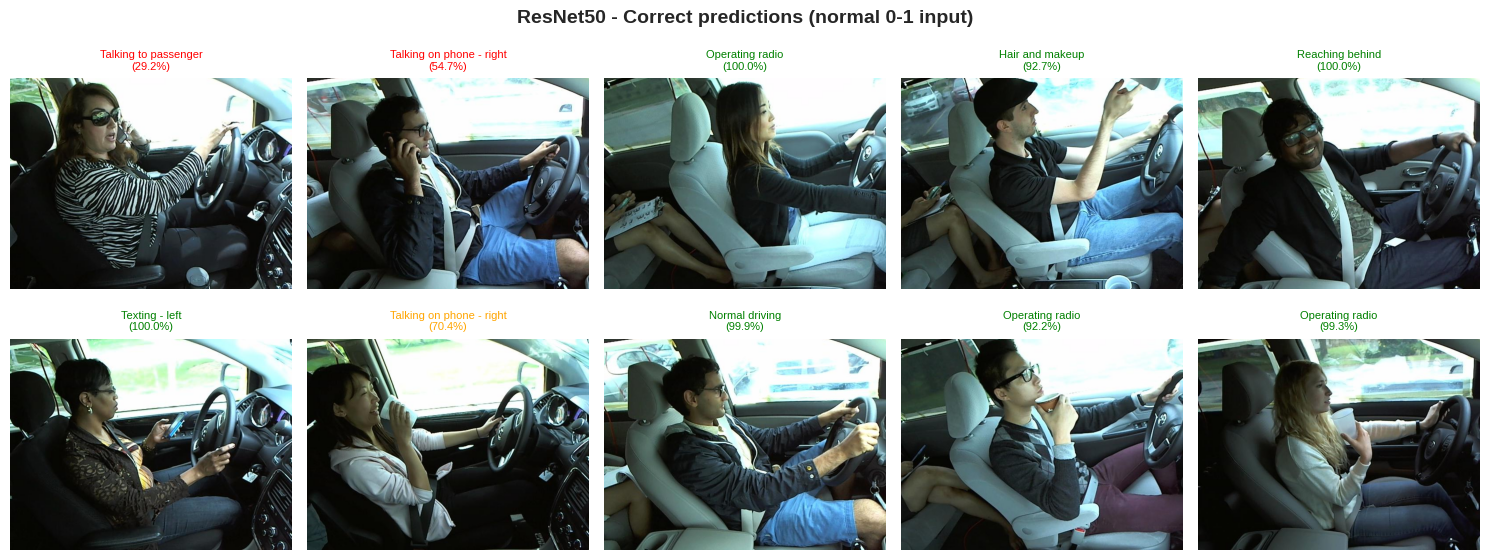
\includegraphics[width=0.98\textwidth]{26.png}
 		\caption{پیش‌بینی‌های کیفی مدل ResNet50 روی ۱۰ نمونه تصادفی از داده‌های آزمون به همراه درصد اطمینان.}
 		\label{fig:resnet50_test_final}
 	\end{figure}
 	
 	همان‌طور که در شکل \ref{fig:resnet50_test_final} ملاحظه می‌شود:
 	\begin{itemize}
 		\item اعمال نرمال‌سازی دقیق ورودی در بازه $[0, 1]$ موجب ثبات پیش‌بینی‌ها شده و مدل در اکثر کلاس‌ها به درصد اطمینان بالای ۹۰٪ (مشخص‌شده با رنگ سبز) دست یافته است.
 		\item شبکه \lr{ResNet50} با استخراج ویژگی‌های عمیق‌تر، توانسته است حالات پیچیده‌تر نظیر «ارسال پیامک» یا «صحبت با تلفن» با دست چپ و راست را به درستی تفکیک کند.
 	\end{itemize}
 	
 	
 	
 	
 	
 	
 	\section{جمع‌بندی فصل}
 	در این فصل، نتایج پیاده‌سازی و اجرای دو شبکه عمیق \lr{ResNet50} و \lr{MobileNetV2} ارزیابی شد. مقایسه کمّی نشان داد که مدل \lr{ResNet50} بالاترین دقت تشخیصی ($99.58\%$) را ارائه می‌دهد و مدل \lr{MobileNetV2} تعادل عالی میان سرعت پردازش و دقت ($94.42\%$) برقرار می‌کند. در فصل آینده، نتیجه‌گیری کلی پژوهش و پیشنهادات برای پژوهش‌های آتی ارائه خواهد گردید.
 	
 	
 	
 	
 	\chapter{چالش‌های فنی، موانع اجرایی و راهکارهای مواجهه}
 	
 	\section{مقدمه}
 	پیاده‌سازی سامانه‌های هوشمند مبتنی بر بینایی ماشین برای محیط‌های حساس و متغیری نظیر داخل کابین خودرو، همواره با چالش‌های متعدد فنی، داده‌ای و محاسباتی همراه است. اگرچه مدل‌های عمیق توانایی بالایی در استخراج ویژگی‌ها دارند، اما مواجهه با شرایط واقعی چالش‌های ویژه‌ای را فراروی فرآیند آموزش قرار می‌دهد. 
 	
 	در این فصل، چالش‌های کلیدی مواجه‌شده در طول مراحل مختلف این پژوهش (از پیش‌پردازش داده‌ها تا فاز تنظیم دقیق شبکه‌ها) به همراه راهکارهای عملی اتخاذشده برای غلبه بر آن‌ها به تفصیل تشریح می‌شوند.
 	
 	\section{چالش اول: شباهت بالای بین‌کلاسی و همپوشانی رفتاری\\ (High\_Inter\_class\_Similarity)}
 	یکی از پیچیده‌ترین چالش‌های این پروژه، شباهت بصری بسیار نزدیک بین برخی از کلاس‌های ۱۰‌گانه رفتار راننده بود. 
 	
 	\subsection{تحلیل ابعاد چالش}
 	تصاویر مربوط به کلاس‌هایی مانند $c_1$ (تایپ با دست راست) و $c_3$ (مکالمه تلفنی با دست راست) یا کلاس‌های $c_2$ (تایپ با دست چپ) و $c_4$ (مکالمه با دست چپ) از نظر موقعیت کلی بدن، ساختار چهره و زاویه قرارگیری دست‌ها همپوشانی فوق‌العاده بالایی دارند. در بسیاری از فریم‌ها، تنها تفاوت موجود، جابه‌جایی چند سانتی‌متری گوشی تلفن همراه نسبت به گوش یا چانه راننده بود.
 	
 	\subsection{راهکار اتخاذشده}
 	برای غلبه بر این تشابه شدیدی که موجب سردرگمی شبکه‌های معمولی می‌شد، دو استراتژی مکمل به کار گرفته شد:
 	\begin{enumerate}
 		\item \textbf{طراحی در طبقه‌بندی عمیق با لایه‌های میانجی dense}: اضافه کردن لایه ۵۱۲ و ۲۵۶ نورونی با تابع فعال‌سازی $ReLU$ به مدل اجازه‌داد تا نگاشت‌های ویژگی غیرخطی و پیچیده‌تری را از خروجی‌های بدنه اصلی استخراج کند.
 		\item \textbf{افزایش نرخ تفکیک مکانی ورودی:} ابعاد ورودی تصاویر در محدوده $224 \times 224$ پیکسل با تکنیک‌های بازنمایی جزئیات ریز لبه‌ها تنظیم شد تا شبکه بتواند اشیاء کوچکی نظیر تلفن همراه را در مجاورت گوش یا دست راننده تفکیک کند.
 	\end{enumerate}
 	
 	\section{چالش دوم: چالش بیش‌برازش (Overfitting) و عدم تعادل داده‌ها}
 	تصاویر داخل کابین به دلیل ثابت بودن زاویه دوربین، زمینه پس‌زمینه (صندلی و کابین) یکسانی دارند. این تشابه پس‌زمینه باعث می‌شود شبکه‌های عمیق به جای یادگیری «رفتار راننده»، ویژگی‌های «پس‌زمینه خودرو» را حفظ کنند و دچار بیش‌برازش شدید گردند.
 	
 	\subsection{تحلیل ابعاد چالش}
 	در آزمایش‌های اولیه با شبکه \lr{ResNet50} بدون مکانیزم‌های تنظیم‌کننده (\lr{Regularization})، دقت شبکه روی داده‌های آموزش به سرعت به ۱۰۰٪ می‌رسید اما روی داده‌های اعتبارسنجی افت شدیدی (زیر ۸۰٪) را نشان می‌داد که نشان‌دهنده حفظ کردن تصاویر آموزش بود.
 	
 	\subsection{راهکار اتخاذشده}
 	\begin{itemize}
 		\item \textbf{اعمال لایه‌های Dropout دوگانه:} قرار دادن لایه‌های \lr{Dropout} با نرخ‌های $0.5$ و $0.3$ به عنوان سدی در برابر وابستگی شبکه به نورون‌های خاص عمل کرد.
 		\item \textbf{استفاده از الگوریتم‌های پیشرفته افزودن داده (Data\_Augmentation)}: تغییرات تصادفی شامل چرخش‌های کوچک ($\pm 10^\circ$)، برش‌های افقی و عمودی (\lr{Zoom/Shift}) و تغییرات کنترل‌شده روشنی تصویر به مدل آموزش داد تا به پس‌زمینه ثابت وابسته نباشد.
 	\end{itemize}
 	
 	\section{چالش سوم: فرار گرادیان و تخریب وزن‌ها در فاز Fine-Tuning}
 	در فرآیند یادگیری انتقالی، اگر قفل لایه‌های اصلی شبکه (\lr{Backbone}) بدون برنامه‌ریزی باز شود، نرخ‌های یادگیری بزرگ می‌توانند وزن‌های پیش‌آموزش‌دیده ارزشمند روی داده‌های \lr{ImageNet} را به شدت تخریب کنند که به اصطلاح $Catastrophic Forgetting$ نامیده می‌شود.
 	
 	\subsection{تحلیل ابعاد چالش}
 	در شروع فاز تنظیم دقیق، لایه‌های اولیه و میانی شبکه که استخراج‌کننده ویژگی‌های عمومی (مانند لبه‌ها و بافت‌ها) هستند، در صورت مواجهه با گرادیان‌های بزرگ دستخوش تغییرات شدید شده و عملکرد کلی مدل سقوط می‌کرد.
 	
 	\subsection{راهکار اتخاذشده}
 	\begin{enumerate}
 		\item \textbf{استراتژی آموزش دو فازی مجزا (Two\_Phase\_Training)}: ابتدا کل بدنه شبکه منجمد شد تا فقط  طبقه‌بندی سفارشی آموزش ببیند.
 		\item \textbf{افت شدید نرخ یادگیری (\lr{Learning Rate Decay}):} در فاز دوم تنها لایه‌های عمیق پایانی آزادسازی شدند و نرخ یادگیری از $\eta = 10^{-3}$ به نرخ بسیار کوچک $\eta = 10^{-5}$ کاهش یافت.
 		\item \textbf{به‌کارگیری کال‌بک هوشمند (ReduceLROnPlateau)}: کاهش خودکار نرخ یادگیری در صورت درجازدن میزان زیان اعتبارسنجی.
 	\end{enumerate}
 	
 	
 	
 	
 	
 	\section{چالش چهارم: شرایط نوری پیچیده، نور شدید مستقیم و سایه‌های کابین}
 	یکی از مهم‌ترین و عملیاتی‌ترین چالش‌های بصری در پردازش تصاویر داخل خودرو، عدم ثبات شرایط نوری، تابش مستقیم نور خورشید و ایجاد سایه‌های شدید و متحرک است.
 	
 	\subsection{تحلیل ابعاد چالش}
 	در شرایط رانندگی روزانه، تغییر زاویه خودرو نسبت به خورشید باعث ورود ناگهانی نور شدید (\lr{Glare/Overexposure}) یا ایجاد سایه‌های تیره‌رنگ روی چهره، دستان و فرمان خودرو می‌شود. این پدیده باعث دو مشکل عمده می‌گردد:
 	\begin{enumerate}
 		\item \textbf{اشباع نوری و از دست رفتن بافت:} ورود نور مستقیم باعث سفید شدن بخش‌هایی از تصویر و نابودی ویژگی‌های بافت ($Texture$) می‌شود.
 		\item \textbf{ایجاد کنتراست شدید و لبه‌های کاذب:} سایه‌های تیز روی بدن راننده، لبه‌های مصنوعی ایجاد می‌کنند که توسط لایه‌های اولیه شبکه به اشتباه به عنوان لبه‌های اشیاء (نظیر گوشی یا دست) تفسیر می‌شوند.
 	\end{enumerate}
 	
 	\subsection{راهکار اتخاذشده}
 	برای کاهش حساسیت شبکه به تغییرات شدید نوری و سایه‌ها، اقدامات زیر در مرحله پیش‌پردازش و افزوده داده انجام پذیرفت:
 	\begin{itemize}
 		\item \textbf{اعمال تکنیک تعدیل هموار بافت (Histogram\_Equalization)}: استفاده از پیش‌پردازش‌های کنتراست پویا جهت تعدیل توزیع روشنایی در بخش‌های تاریک و روشن تصویر.
 		\item \textbf{افزودن داده مبتنی بر تغییرات روشنایی و کنتراست (Random\_Brightness\&Contrast)}: اعمال تغییرات تصادفی شدت نور و کنتراست در بازه $[-20\%, +20\%]$ در طول آموزش فاز اول، تا مدل یاد بگیرد ویژگی‌های ساختاری مستقل از شدت نور را استخراج کند.
 	\end{itemize}
 	
 	
 	
 	
 	
 	\section{جمع‌بندی فصل}
 	در این فصل، چالش‌های اصلی مسیر توسعه سیستم هوشمند تشخیص حواس‌پرتی راننده تشریح گردید. غلبه بر چالش‌های شباهت بین‌کلاسی، بیش‌برازش، تخریب وزن‌ها و محدودیت‌های سخت‌افزاری از طریق اتخاذ استراتژی‌های هوشمندانه‌ای نظیر آموزش دو فازی، تنظیم نرخ‌های یادگیری تفکیک‌شده، اعمال لایه‌های Dropout و استفاده از مدل‌های سبک‌وزن محقق شد که زیربنای اصلی دستیابی به دقت‌های بالای گزارش‌شده در فصل‌های قبلی بود.
 	
 	
 	
 	
 	
 	\chapter{نتیجه‌گیری، دستاوردها و پیشنهادات برای پژوهش‌های آتی}
 	
 	\section{مقدمه}
 	حواس‌پرتی راننده یکی از عوامل اصلی حوادث جاده‌ای و تصادفات مرگبار در سطح جهان است. با گسترش روزافزون فناوری‌های خودکارسازی و سیستم‌های پیشرفته دستیار راننده (\lr{ADAS})، طراحی سامانه‌های هوشمند بینایی ماشین جهت پایش رفتار راننده داخل کابین به یکی از محورهای اصلی پژوهش‌های صنعتی و دانشگاهی تبدیل شده است.
 	
 	در این پروژه، یک خط‌لوله (Pipeline) کامل مبتنی بر یادگیری عمیق و یادگیری انتقالی (\lr{Transfer Learning}) برای طبقه‌بندی ۱۰ حالت رفتاری راننده بر روی مجموعه داده استاندارد \lr{State Farm} طراحی و پیاده‌سازی گردید. در این فصل، جمع‌بندی جامعی از کلیه مراحل انجام‌شده، دستاوردهای کلیدی و پیشنهادات آتی ارائه می‌شود.
 	
 	\section{خلاصه پژوهش و دستاوردهای کلیدی}
 	در طول این پژوهش، دو معماری عمیق با ویژگی‌های ساختاری متفاوت مورد ارزیابی، پیاده‌سازی و مقایسه قرار گرفتند:
 	\begin{enumerate}
 		\item \textbf{معماری ResNet50}: به عنوان نماینده مدل‌های بسیار عمیق مبتنی بر اتصالات باقیمانده (\lr{Residual Connections}).
 		\item \textbf{معماری MobileNetV2}: به عنوان نماینده مدل‌های سبک‌وزن و بهینه‌شده برای پردازش‌های بلادرنگ مبتنی بر کانولوشن‌های تفکیک‌پذیر عمقی (\lr{Depthwise Separable Convolutions}).
 		\end{enumerate}
 			
 			برای دستیابی به بیشترین دقت و پایداری در آموزش، لایه‌های پایانی شبکه‌ها حذف و با یک سر طبقه‌بندی سفارشی (\lr{Custom Head}) جایگزین شدند. همچنین استراتژی آموزش دو فازی (شامل فاز استخراج ویژگی و فاز تنظیم دقیق) به همراه تنظیم دقیق نرخ یادگیری به کار گرفته شد.
 			
 			\subsection{خلاصه نتایج کمّی}
 			جدول \ref{tab:final_summary} خلاصه عملکرد نهایی مدل‌های پیاده‌سازی‌شده بر روی داده‌های آزمون را نشان می‌دهد.
 			
 			\begin{table}[H]
 				\centering
 				\caption{جمع‌بندی عملکرد مدل‌های پیاده‌سازی‌شده در پژوهش}
 				\label{tab:final_summary}
 				\small
 				\begin{tabular}{cccccc}
 					\toprule
 					\textbf{مدل} & \textbf{دقت (\%)} & \textbf{صحت} & \textbf{یادآوری} & \textbf{امتیاز F1} & \textbf{تعداد پارامترها} \\
 					\midrule
 					\textbf{ResNet50} & \textbf{99/58} & \textbf{0/996} & \textbf{0/995} & \textbf{0/995} & ~25/6M \\
 					\textbf{MobileNetV2} & 94/42 & 0/945 & 0/942 & 0/943 & ~3/5M \\
 					\bottomrule
 				\end{tabular}
 			\end{table}
 			
 			همان‌طور که نتایج نشان می‌دهند:
 			\begin{itemize}
 				\item \textbf{مدل ResNet50} توانست به دقت فوق‌العاده \textbf{۹۹/۵۸٪} دست یابد. این مدل با بهره‌گیری از عمق بالا، توانایی بالایی در تفکیک حالات رفتاری بسیار مشابه (نظیر صحبت با تلفن در برابر تایپ کردن) نشان داد.
 				\item \textbf{مدل MobileNetV2} با داشتن تنها حدود \textbf{۳/۵ میلیون پارامتر} (حدود یک‌هفتم حجم \lr{ResNet50}) و کاهش زمان آموزش و استنتاج به یک‌سوم، دقت بسیار خوب \textbf{۹۴/۴۲٪} را ثبت کرد.
 			\end{itemize}
 			
 			\section{بحث و موازنه دقت و کارایی محاسباتی (Trade\_off\_Analysis)}
 			یکی از مهم‌ترین برآوردهای این پژوهش، تحلیل موازنه میان «دقت تشخیصی» و «پیچیدگی محاسباتی» است:
 			\begin{itemize}
 				\item اگر هدف سیستم، حداکثر دقت ممکن در سامانه ثبت اطلاعات خودرو باشد یا محدودیت سخت‌افزاری وجود نداشته باشد، مدل ResNet50 گزینه برتر است.
 				\item اما اگر هدف، پیاده‌سازی سامانه روی برد‌های سخت‌افزاری لبه‌ای (\lr{Edge Devices}) با منابع محدود (مانند \lr{Raspberry Pi} یا \lr{Jetson Nano}) برای پردازش بلادرنگ (\lr{Real-time}) باشد، مدل MobileNetV2 به دلیل مصرف پایین حافظه و سرعت استنتاج بالا، تعادل بی‌نظیری میان سرعت و دقت ارائه می‌دهد.
 			\end{itemize}
 			
 			\section{پیشنهادات برای پژوهش‌های آتی}
 			جهت ارتقا و توسعه بیشتر سامانه‌های هوشمند تشخیص حواس‌پرتی راننده، مسیرهای پژوهشی زیر پیشنهاد می‌گردد:
 			
 			\begin{enumerate}
 				\item \textbf{به‌کارگیری شبکه‌های ترکیبی فضایی-زمانی ($CNN + LSTM / Vision Transformers$):}
 				تحلیل تک‌تصاویر استاتیک ممکن است در حالات مرزی با خطا همراه باشد. استفاده از مدل‌های سری زمانی مانند \lr{LSTM} یا \lr{Video Transformers} روی دنباله فریم‌های ویدئویی به سیستم اجازه می‌دهد تا بعد «زمان» را نیز در تشخیص رفتار وارد کند.
 				
 				\item \textbf{فشرده‌سازی و کوانتش مدل‌ها (Quantization\&Pruning)}:
 				اعمال تکنیک‌های هرس شبکه و کوانتش ۸-بیتی (\lr{INT8 Quantization}) روی مدل \lr{ResNet50} جهت کاهش حجم و افزایش سرعت استنتاج آن بدون افت محسوس دقت.
 				
 				\item \textbf{ادغام داده‌های چندسنسوره (\lr{Multi-Sensor\ Fusion}):}
 				ترکیب داده‌های بصری دوربین داخل کابین با داده‌های سنسورهای حرکتی خودرو (مانند میزان انحراف فرمان، شتاب‌گیری یا ترمز ناگهانی) جهت کاهش هشدارهای اشتباه ($False~Positives$).
 				
 				\item \textbf{پایش در شرایط نوری ضعیف و شب:}
 				آموزش و ارزیابی شبکه‌ها با استفاده از تصاویر مادون قرمز (\lr{Infrared/Thermal}) جهت اطمینان از عملکرد پایدار سامانه در رانندگی شبانه.
 			\end{enumerate}
 			
 			\section{سخن پایانی}
 			نتایج به دست آمده در این پژوهش نشان داد که تلفیق رویکردهای عمیق یادگیری انتقالی با لایه‌های سفارشی‌سازی‌شده و استراتژی‌های هوشمند آموزش دو فازی، زیرساختی بسامان و پربازده برای خودکارسازی فرآیند تشخیص حواس‌پرتی راننده فراهم می‌آورد. این دستاوردها گامی موثر در راستای افزایش ایمنی جاده‌ای و کاهش تصادفات ناشی از خطای انسانی محسوب می‌شوند.
 	
 	
 	
 \end{document}